\documentclass[12pt, a4paper, titlepage]{report}
\usepackage[spanish]{babel}
\usepackage[utf8]{inputenc}
\usepackage[linesnumbered,lined,boxed,commentsnumbered]{algorithm2e}
\usepackage{float}
\usepackage{subfig}
%%Imágenes
\usepackage{graphicx}
%%Colores de texto 
\usepackage{xcolor}
\usepackage{colortbl}
%%Links
\usepackage[hidelinks]{hyperref}
%%Comentarios
\usepackage{verbatim}
%%PARA IMÁGENES EN LÍNEA
\newcommand*{\img}[1]{%
    \raisebox{-.3\baselineskip}{%
        \includegraphics[
        height=1cm,
        width=2cm,
        keepaspectratio,
        ]{#1}%
    }%
}

%---------------------------GLOSARIO----------------------------%
\usepackage{glossaries}
\makeglossaries

\newglossaryentry{Flash}
{
    name=Flash,
    description={Aplicación informática englobada en la categoría de reproductor multimedia}
}
\newglossaryentry{NetScape}{
    name=Netcape,
    description={Navegador web de la compañia NetScape Communications}
}
\newglossaryentry{cookies}{
    name=Cookies,
    description={Es una pequeña información enviada por un sitio web y almacenada en el navegador del usuario, de manera que el sitio web puede consultar la actividad previa del navegador.
    Sus principales funciones son recordar accesos y
    conocer información sobre los hábitos de navegación e intentos de spyware}
}

\newglossaryentry{HMACSHA14}{
    name=HMACSHA14,
    description={HMAC-SHA1 es un tipo de algoritmo o herramienta que provee un algoritmo estandar MAC.}
}

\newglossaryentry{backdoor}{
    name=Backdoor,
    description={Una puerta trasera o backdoor es una secuencia especial dentro del código de programación, mediante la cual se pueden evitar los sistemas de seguridad del algoritmo (autentificaci\'on) para acceder al sistema. Aunque estas puertas pueden ser utilizadas para fines maliciosos y espionaje no siempre son un error, ya que pueden haber sido diseñadas con la intención de tener una entrada secreta}
}

\newglossaryentry{Robo de Identidad}{
    name=Identity theft,
    description={También conocido como ''robo de identidad'' se produce cuando una persona adquiere, transfiere, posee o utiliza información personal de una persona física o jurídica de forma no autorizada, con la intención de efectuar o vincularlo con algún fraude u otro delito}
}
%\acrlong{}  \acrshort{} 
\newacronym{html}{HTML}{Hyper Text Markup Languaje}
\newacronym{iu}{IU}{Interfaz de Usuario}
\newacronym{http}{HTTP}{Hypertext Transfer Protocol}
\newacronym{css}{CSS}{Cascading Style Sheets}
\newacronym{url}{URL}{Uniform Resource Locator}
\newacronym{id}{ID}{identificador}

%------------------FINAL DE GLOSARIO-----------------------%

%------------------ESTABLECER COLORES----------------------%
\definecolor{guindapoli}{RGB}{102, 0, 51}
\definecolor{azulescom}{RGB}{0, 0, 102}
\definecolor{azulclaro}{RGB}{222, 232, 255}
\definecolor{azulfuerte}{RGB}{60, 150, 250}
%------------------FIN DE COLORES------------------%
\begin{document}
	
	%PARA QUE DETECTE HASTA SUBSUBSECTION
	\setcounter{secnumdepth}{3}
	
	%PORTADA
	\begin{titlepage}	
		
		\vspace*{-1.5in}
		
		\begin{figure}[htb]
	    \begin{minipage}{0.5\textwidth}
        %    \centering
            
\includegraphics[width=0.8\textwidth]{imagenes/MarcoTeorico/logoipn.png}
        \end{minipage}%
        \hspace{5mm}
        \begin{minipage}{0.5\textwidth}
        %    \centering
            
\includegraphics[width=0.8\textwidth]{imagenes/MarcoTeorico/logoescom.png}
        \end{minipage}
		\end{figure}
		
		\begin{center}
			
			\begin{LARGE}
				\textcolor{guindapoli}{INSTITUTO POLITÉCNICO NACIONAL}\\
			\end{LARGE}	
			
			\vspace*{0.2in}
			
			\begin{Large}
				\textcolor{azulescom}{ESCUELA SUPERIOR DE CÓMPUTO}\\
			\end{Large}		
			
			\vspace*{0.4in}
			
			\begin{large}
				Trabajo Terminal I.\\
			\end{large}
			
			\vspace*{0.2in}
			
			\begin{Large}
				\textbf{Autentificación mediante Chaffing and Winnowing en el protocolo HTTP}\\
			\end{Large}
			
			\vspace*{0.2in}
			
			\begin{large}
				2018-B003.\\
			\end{large}
			
			\vspace*{0.2in}
			
			\rule{80mm}{.1mm}\\
			\vspace*{0.1in}
			
			\begin{large}
				\begin{center}
					Integrantes:\\
					Blancas Pérez Bryan Israel\\
					Carrillo Fernández Gerardo\\
					Morales González Diego Arturo\\
					Paredes Hernández Pedro Antonio\\
				\end{center}
			\end{large}
			
			\begin{large}
				Directores:\\
				Moreno Cervantes Axel Ernesto\\
				Díaz Santiago Sandra\\
			\end{large}
			
		\end{center}
	
	\end{titlepage}

    %Índice
	\begin{appendix}
		\renewcommand*\contentsname{{\textcolor{azulescom}{Índice.}}}
		\tableofcontents
		\newpage
		%%índice de figuras
		\renewcommand*\listfigurename{{\textcolor{azulescom}{Índice de figuras.}}}
		\listoffigures
		\newpage
		%%Índice de tablas
		\newpage
		\renewcommand*\listtablename{{\textcolor{azulescom}{Índice de cuadros.}}}
		\listoftables
		
		\newpage
		\renewcommand*\glossaryname{{\textcolor{azulescom}{Glosario.}}}
		
		\printglossary
	\end{appendix}
	
    \textcolor{guindapoli}{\part{Trabajo Terminal I}}
    
    \renewcommand\thechapter{\arabic{chapter}}
    \renewcommand{\appendixname}{Capítulo}
    \chapter{\textcolor{azulescom}{Introducción}}

	\renewcommand\thesection{\arabic{section}}	
	%\section{Introducción.}
		
		En la actualidad la mayor\'ia de los usuarios de internet necesitan guardar contraseñas para sus distintas cuentas en las diferentes páginas web a las que ingresan, ya que recordarlas es un problema debido a la gran cantidad de servicios que se utilizan. Como consecuencia de que la autentificaci\'on por contraseña es la más utilizada en los servicio web hoy en día \cite{ComparisonAuthenticationMethodsResources}, los distintos servicios web han implementado mecanismos de seguridad tales como contraseñas que contengan un mínimo de caracteres determinados, al menos un caracter especial, entre otros. Esto ha provocado que éstas sean más difíciles de recordar y han orillado a los usuarios a optar por guardarlas en medios físicos o digitales para recordarlas cuando sea necesario. 
		Sin embargo, perder esas claves (principalmente con los medios físicos) presenta un grave problema de seguridad, teniendo como consecuencia: perdida de datos sensibles, robo de identidad, robo de cuentas bancarias, etc.\\
		
		La gran mayoría de servicios web han implementado la función "recordar contraseña", la cual hace que el usuario no tenga que ingresar sus credenciales\footnote{Credenciales se entiende como los datos que un servicio web requiere para poder acceder al él. Comúnmente son 'usuario' y 'contraseña'.} cada vez que se quiere acceder al servicio. Esta función por lo general hace uso de cookies que es información almacenada en el explorador web del usuario, esto representa una amenaza de seguridad ya que permite rastrear la información de navegación del usuario y puede ser muy útil para sitios fraudulentos o se puede presentar un robo de cookies con el cual los intrusos podrían hacerse pasar como el usuario, entre otros problemas que \'estas representan.
	    
	    %El método Chaffing and Winnowing proporciona confidencialidad de los mensajes sin la necesidad de cifrados o el uso de estenografía, aunque no cumple los demás objetivos de criptografía, pero si lo combinamos con algún cifrado asimétrico proporciona un nivel de seguridad muy alto que es lo que pretendemos en este trabajos.
	    
	    El método \textit{Chaffing and Winnowing} proporciona confidencialidad de los mensajes sin la necesidad de usar métodos de cifrado o esteganografía, agregando 'basura' (\textit{Chaffing}) para que el mensaje quede ininteligible ante la vista de terceros no implicados en la comunicación, y sólo el receptor pueda 'limpiar' (\textit{Winnowing}) el mensaje obteniendo la información relevante.
	    
		Es por ello que en este trabajo terminal se propone realizar un nuevo método de autentificación por medio del método de \textit{Chaffing and Winnowing} y con la ayuda de una extensión de Google Chrome, la cual servirá para la inyección del certificado de autentificación en el protocolo HTTP, emitido por un servidor autentificador, que el usuario obtendrá al iniciar sesión una única vez en la extensión. Así, si un servicio web tiene este tipo de autentificación disponible, lo podrá validar. El propósito principal de este trabajo es que los usuarios puedan realizar un inicio de sesión más cómodo, seguro y sin la necesidad de recordar sus distintas contraseñas constantemente.
		
		
	\section{Objetivos.}
		\subsection{Objetivo general. }
			%Realizar una extensión en Google Chrome que modifique los datos del protocolo \acrshort{http}, para permitir que el servidor detecte el método de autentificación propuesto basado en \textit{Chaffing and Winnowing}.\\
			Realizar un nuevo método de autenticación modificando los datos del protocolo HTTP utilizando Chaffing and Winnowing con la ayuda de una extensión del navegador Google Chrome.
		\subsection{Objetivos particulares.}
			\begin{itemize}
				\item Investigar e implementar el desarrollo de extensiones en Google Chrome.
				\item Investigar sobre los mecanismos de autentificación.
				\item Investigar sobre la técnica de \textit{Chaffing and Winnowing} para adaptar su implementación.
				\item Inyectar el código (\textit{Chaffing}) en el encabezado HTTP para enviar la petición al servidor. 
				\item Implementación de un Login en la extensión de Google Chrome.
				\item Investigar sobre Autoridades Certificadoras para implementar un servidor autentificador
				\item Generación de certificado autentificador del usuario
				\item Implementación de un servicio web de prueba.
				\item Desarrollo de un API para nuestro servidor que obtenga el certificado del usuario (\textit{Winnowing}).
				\item Modificar el código del servidor Apache para simular y comprobar el funcionamiento de la extensión. 
				\item Realizar pruebas de seguridad para comprobar la eficacia de la extensión. 
			\end{itemize}
			
	\section{Justificación.}
	    Los usuarios de Internet, han optado por guardar sus contraseñas en medios físicos o digitales, lo cual presenta un problema grave de seguridad ya que la pérdida o acceso a uno de estos medios, significaría el acceso a todos los servicios guardados en éstos. Ante esto, la gran mayoría de los servicios web, han implementado una solución al problema de recordar las credenciales y lo tedioso de tener que ponerlas cada vez que se desea acceder, la cual es recordar tu usuario y contraseña, para que automáticamente puedas acceder al servicio. Dicha solución presenta un problema de seguridad, ya que los archivos en donde se guarda la información se pueden copiar y con ello replicarlos en cualquier otra computadora.\\
	    
        Tenemos también algunas opciones que los navegadores y servicios nos ofrecen como el de “recordar contraseña”, sin embargo, estos métodos no son del todo seguros para los usuarios, por ejemplo, la configuración de Google Chrome nos permite observar todas las contraseñas de las diferentes páginas a las que hemos accedido sin ninguna especie de autentificación de quién accede a estas contraseñas, lo cual supone un claro riesgo a la integridad del dueño de estas cuentas.\\
        
        Es por ello, que este proyecto busca beneficiar al usuario evitando que tenga que ingresar sus credenciales continuamente, y sin que el sistema tenga que guardar las credenciales del servicio web que el usuario use. Por lo tanto, este proyecto brinda una alternativa segura de autentificación en un servicio web. \\
	    \newpage
	    
	\section{Metodolog\'ia.}
		El proceso de desarrollo que seguiremos estará basado en la metodología de prototipos evolutivos, el cual consiste en la implementación parcial del proyecto cumpliendo con los requerimientos que van surgiendo a lo largo del desarrollo, de esta manera es posible ir experimentando con un prototipo parcialmente funcional e identificar posibles mejoras o fallas con el fin de lograr el objetivo final.
		Esta metodología está compuesta por las siguientes fases:
		\begin{itemize}
		    \item Fase de investigación preliminar.
		    \item Especificación de requerimientos y prototipos
		    \item Diseño técnico
		    \item Programación y pruebas
		    \item Operación y mantenimiento
		\end{itemize}
		
        
        Primero tendremos la fase de “investigación preliminar”, donde se van a definir las metas principales, después en la fase de “especificación de requerimientos y prototipos", se hace el diseño básico para dar paso a la creación del primer prototipo correspondiente, y después verificar el cumplimiento de los requerimientos y de ser necesario modificarlo hasta que los cumpla. En la tercera fase (diseño técnico) se realiza un diseño detallado y la documentación necesaria para que en la cuarta fase (programación y pruebas) se implemente y se pruebe el prototipo. Finalmente, en la última fase (Operación y mantenimiento) se hace la liberación y el mantenimiento del prototipo final.
        
        Para nuestro proyecto realizaremos 4 prototipos, los cuales son: 
        \begin{enumerate}
            \item Creación de extensión de Google Chrome para interceptar la petición \acrshort{http}. 
            \begin{itemize}
                \item Investigación preliminar: 
                \begin{itemize}
                    \item Investigar sobre el desarrollo de extensiones en Google Chrome.
                \end{itemize}
                \item Especificación de requerimientos y prototipos:
                \begin{itemize}
                    \item Ejecución de la extensión sobre Google Chrome.
                    \item Detectar petición \acrshort{http} e interceptarla.
                    \item Subir archivo autentificador a la extensión.
                \end{itemize}
                \item Diseño técnico: 
                \begin{itemize}
                    \item Documentación del prototipo.
                \end{itemize}
                \item Documentación del prototipo.
                \begin{itemize}
                    \item Desarrollo de la extensión.
                    \item Pruebas de la extensión.
                \end{itemize}
            \end{itemize}
            \item Inyección de código autentificador (Chaffing) en el encabezado \acrshort{http}. 
            \begin{itemize}
                \item Investigación preliminar: 
                \begin{itemize}
                    \item Investigación sobre el método Chaffing and Winnowing. 
                \end{itemize}
                \item Especificación de requerimientos y prototipos: 
                \begin{itemize}
                    \item  Lectura del archivo autentificador.
                    \item  Análisis del protocolo \acrshort{http}. 
                    \item  Inyección del código autentificador sobre el protocolo \acrshort{http}.
                    \item Mandar petición a servidor.
                \end{itemize}
                \item Diseño técnico:
                \begin{itemize}
                    \item Documentación del prototipo. 
                \end{itemize}
                \item Programación y pruebas: 
                \begin{itemize}
                    \item Desarrollo del complemento de la extensión. 
                    \item Creación del algoritmo de inyección de código. 
                    \item Pruebas de la extensión. 
                \end{itemize}
            \end{itemize}
            \item Modificación del servidor Apache para recibir el protocolo con la inyección de código.
            \begin{itemize}
                \item  Investigación preliminar: 
                \begin{itemize}
                    \item Investigación sobre el servidor Apache.
                    \item Analizar la arquitectura del servidor Apache
                    \item Investigación sobre la versión conveniente a modificar.
                \end{itemize}
                \item Especificación de requerimientos y prototipos: 
                \begin{itemize}
                    \item Recibir petición \acrshort{http} de la extensión. 
                    \item  Detectar el tipo de autentificación que se usará.
                \end{itemize}
                \item Diseño técnico: 
                \begin{itemize}
                    \item Documentación del prototipo.
                \end{itemize}
                \item Programación y pruebas:
                \begin{itemize}
                    \item Descargar la versión del servidor Apache a usar.
                    \item Modificación del código del servidor Apache para detectar el tipo de autentificación que se usará. 
                    \item Pruebas de funcionamiento.
                \end{itemize}
            \end{itemize}
            \item Realización de la autentificación (Winnowing) en el servidor para realizar el login.
            \begin{itemize}
                \item Investigación y pruebas
                \begin{itemize}
                    \item  Investigar sobre la implementación de autenticador en distintos servidores 
                \end{itemize}
                \item Especificación de requerimientos y prototipos:
                \begin{itemize}
                    \item Recibir la petición.
                    \item Descifrar la petición.
                    \item Dar respuesta al usuario.
                \end{itemize}
                \item Diseño técnico:
                \begin{itemize}
                    \item Documentación del prototipo. 
                \end{itemize}
                \item Programación y pruebas:
                \begin{itemize}
                    \item Creación de algoritmo que obtenga el código autentificador del protocolo \acrshort{http}.
                    \item Verificación del código autentificador.
                    \item Responder al usuario.
                    \item Pruebas de funcionamiento.
                \end{itemize}
            \end{itemize}
        \end{enumerate}
		% \subsection{Estado del Arte.}
	
	\chapter{\textcolor{azulescom}{Marco teórico}}
	    
	    %   %   %   %   %   %   %   %   %   
		%		                        %
		%           INTRODUCCIÓN        %
		%                               %
	    %   %   %   %   %   %   %   %   %
	    \section{Introducci\'on.}
	        Dado que este Trabajo terminal relaciona tem\'aticas muy enfocadas a la seguridad y aspectos web, es necesario conocer algunos conceptos e ideas fundamentales tanto para entender el trabajo como para conocer su funcionamiento, por lo tanto será necesario hablar de m\'etodos de autenticación, concepto, objetivos, aplicaciones y tipos de criptografía así como el método de Chaffing and Winnowing que es la parte interesante de todo este trabajo; en este marco teórico tratamos de explicar de manera breve y con un enfoque directo al uso que le daremos en el desarrollo del proyecto.
	    %   %   %   %   %   %   %   %   %   
		%		                        %
		%   MÉTODOS DE autentificación    %
		%                               %
	    %   %   %   %   %   %   %   %   %
	    \section{Métodos de autententicación en internet.}
	    \paragraph{}Con la evolución de la web, distintas páginas ofrecen ciertos servicios a los usuarios y con la finalidad de dar una experiencia óptima y segura, se requiere que una persona o usuario se identifique para el uso de estos servicios, es aquí donde entra en juego el papel de los métodos de autentificación. Para poder asegurar la confidencialidad de la información manejada en todos estos servicios, es necesario restringir el acceso de este, para esto se utiliza la identificación y la autenticación; la identificación es un procedimiento donde el sujeto es reconocido por algún \acrshort{id}, esto es equivalente al saber una parte de información en específico, mientras que la autenticación es el proceso de validación de si el sujeto es la persona quien dice ser al tratar de identificarse.\cite{articuloAxel}\\
	    
	    Para probar una identidad, el sujeto presenta algo llamado "factor de autenticación", principalmente existen 4: 
	    \begin{itemize}
	        \item El sujeto tiene algo (Token, documento, un material específico, etc.).
	        \item El sujeto conoce algo (contraseña, login, respuesta a una pregunta, etc.).
	        \item El sujeto tiene una característica biológica (huella dactilar, ADN, etc.).
	        \item El sujeto se encuentra en un lugar en específico (dirección IP, información de un lugar en específico, etc.).
	    \end{itemize}
	    Hoy en  día, la autenticación por contraseña es el método más utilizado, más que otra cosa por su ventaja principal: su simplicidad de utilización, sin embargo, así como tiene una gran ventaja, la autenticación por contraseña también tiene muchos problemas y desventajas de seguridad.
	    
	    A continuación, mostraremos algunas tablas comparativas que serviran para tener una mejor perspectiva de las ventajas,d esventajas, vulnerabilidades de los diferentes métodos de autenticación, entre otras cosas:
		
		\begin{table}[H]
			\centering
			\resizebox{13cm}{!} {
				\begin{tabular}{l|l|l|l|l|l|l|l|}
					\cline{2-8}
					& Recordar & \begin{tabular}[c]{@{}l@{}}Otros\\ dispositivos\end{tabular} & Acciones & Facilidad & Tiempo & Errores & Recuperación \\ \hline
					\multicolumn{1}{|l|}{Contraseñas}                                                      & 1        & 3                                                            & 2        & 3         & 3      & 2       & 3            \\ \hline
					\multicolumn{1}{|l|}{Otros recursos}                                                   & 2        & 3                                                            & 3        & 3         & 3      & 3       & 2            \\ \hline
					\multicolumn{1}{|l|}{\begin{tabular}[c]{@{}l@{}}Contraseñas \\ gráficas\end{tabular}}  & 1        & 1                                                            & 2        & 3         & 3      & 2       & 3            \\ \hline
					\multicolumn{1}{|l|}{\begin{tabular}[c]{@{}l@{}}Contraseñas \\ dinámicas\end{tabular}} & 1        & 3                                                            & 2        & 2         & 3      & 2       & 2            \\ \hline
					\multicolumn{1}{|l|}{Tokens}                                                           & 3        & 1                                                            & 1        & 2         & 2      & 3       & 1            \\ \hline
					\multicolumn{1}{|l|}{Multivariación}                                                   & 1        & 1                                                            & 1        & 3         & 2      & 2       & 1            \\ \hline
					\multicolumn{1}{|l|}{Cryptografía}                                                     & 3        & 1                                                            & 1        & 1         & 1      & 2       & 1            \\ \hline
					\multicolumn{1}{|l|}{Biométricos}                                                      & 3        & 3                                                            & 2        & 3         & 2      & 2       & 1            \\ \hline
				\end{tabular}
			}
			\caption{Tabla comparativa de la aplicación en los distintos métodos de autentificaci\'on}
		\end{table}
		La tabla anterior concentra las siguientes características:
		
		\begin{itemize}
			\item Recordar: Hace referencia a que tan complicado es que un usuario se acuerde de los datos necesarios para la autentificaci\'on. 
			\item Otros dispositivos: El usuario usa una entidad externa para facilitar su autentificaci\'on.
			\item Acciones: Hace referencia a que tantas acciones adicionales se deben de realizar para autentificarse.
			\item Facilidad: Simplicidad de tecnología.
			\item Tiempo: Cantidad de recursos temporales que consume el método de autentificaci\'on.
			\item Errores: Posibles errores durante la autentificaci\'on. 
			\item Recuperación: Denota la dificultad de recuperar la clave de acceso en caso de pérdida.
		\end{itemize}
		
		En el cuadro No.2 se muestra una tabla comparativa del nivel de seguridad en los distintos métodos de autentificaci\'on, donde 1 - baja seguridad, 2 – media seguridad y 3 – alta seguridad.
		
		\begin{table}[H]
			\centering
			\resizebox{10cm}{!} {
				\begin{tabular}{l|l|l|l|l|}
					\cline{2-5}
					& \begin{tabular}[c]{@{}l@{}}Ataque por\\ fuerza bruta\end{tabular} & Observación & \begin{tabular}[c]{@{}l@{}}Hackeo\\ indirecto\end{tabular} & Phishing \\ \hline
					\multicolumn{1}{|l|}{Contraseñas}                                                      & 1                                                                 & 1           & 1                                                          & 1        \\ \hline
					\multicolumn{1}{|l|}{Otros recursos}                                                   & 2                                                                 & 2           & 3                                                          & 3        \\ \hline
					\multicolumn{1}{|l|}{\begin{tabular}[c]{@{}l@{}}Contraseñas \\ gráficas\end{tabular}}  & 1                                                                 & 1           & 2                                                          & 2        \\ \hline
					\multicolumn{1}{|l|}{\begin{tabular}[c]{@{}l@{}}Contraseñas \\ dinamicas\end{tabular}} & 2                                                                 & 3           & 2                                                          & 2        \\ \hline
					\multicolumn{1}{|l|}{Tokens}                                                           & 3                                                                 & 3           & 3                                                          & 3        \\ \hline
					\multicolumn{1}{|l|}{Multivariación}                                                   & 1                                                                 & 1           & 3                                                          & 3        \\ \hline
					\multicolumn{1}{|l|}{Cryptografía}                                                     & 3                                                                 & 3           & 3                                                          & 3        \\ \hline
					\multicolumn{1}{|l|}{Biométricos}                                                      & 3                                                                 & 3           & 1                                                          & 1        \\ \hline
				\end{tabular}
			}
			\caption{Tabla comparativa de la seguridad en los distintos métodos de autentificaci\'on}
		\end{table}
		La tabla se enfoca principalmente en los siguientes problemas de seguridad: 
		
		\begin{itemize}
			\item Ataque por fuerza bruta: Se descifra el método de autentificaci\'on con una gran cantidad de intentos, usualmente generados por un programa.
			\item Observación: Cuando se intenta ver directamente los datos necesarios para la autentificaci\'on desde una distancia cercana hasta incluso usando binoculares, cámaras o algún otro dispositivo.
			\item Hackeo indirecto: El usuario confía sus datos del método de autentificaci\'on a terceros quienes pueden ser atacados. 
			\item Phishing: Hace referencia a programas que se hacen pasar por entidades confiables para interceptar los datos que desean.
		\end{itemize}
		
	    \textbf{Seguridad en internet}
	    En la actualidad, el incremento constante de internet ha impactado directamente en la seguridad de la información que se maneja cotidianamente y por la mayoría de usuarios. Existen infinidad de sitios donde es aplicada la seguridad, ya que sin ésta, se verían afectados todos los usuarios en  sus cuentas, pudiendo verse afectados desde un posible \Gls{Robo de Identidad} (Robo de identidad), hasta la perdida de dinero real dado que la base de algunas de éstas paginas son E-Commerce, estas paginas implican el manejo de tarjetas de crédito, paypal, etc.\\
		
		Uno de los puntos más críticos de la seguridad en Internet son las herramientas que interactúan de forma directa con los usuarios. Es común escuchar sobre fallas en los sistemas de protección de los servidores más frecuentemente utilizados, por ejemplo Apache, NGINX, IIS, etc. O en los lenguajes de programación en que son escritas las aplicaciones. \cite{refSeguridadWeb} Sin embargo, la vulnerabilidad más grande dentro de un sistema, son los ataques directos a los usuarios finales durante la autentificación.\\
	    
	    \subsection{Coockies. }
		Durante la navegación por internet, la información sobre la computadora puede ser colectada y almacenada. Ésta puede ser de carácter general sobre el equipo y puede ser también información más específica sobre los hábitos de navegación del usuario, toda esta información guardada se le conoce como \Gls{cookies}\cite{refCookies}. \\
		A continuación se muestran los diferentes tipos de cookies que existen para los navegadores.
		
		\begin{itemize}
		    \item \textbf{Cookies propias:} Las cookies se gestionan desde el terminal o dominio de un mismo editor.
		    \item \textbf{Cookies de terceros:} Las cookies no son enviadas por el propio editor, sino por otra entidad.  
		    \item \textbf{Cookies de sesión:} Los datos recabados sólo se recogen mientras el usuario está navegando por la página web.
		    \item \textbf{Cookies persistentes:} Los datos continúan almacenados en el terminal y se puede acceder a ellos durante un periodo de tiempo determinados.
		    \item \textbf{Cookies técnicas:} Permiten controlar el tráfico y la comunicación de datos.		
            \item \textbf{Cookies de personalización:} Dejan a los usuarios acceder según algunas características propias que se recogen (navegador, idioma, etc.).
            \item \textbf{Cookies de análisis:} Recogen datos sobre el comportamiento de los usuarios y permiten elaborar un perfil de usuario.
            \item \textbf{Cookies publicitarias:} Recogen datos sobre la gestión de los espacios publicitarios.
        \end{itemize}
		
		Las cookies persistentes son aquellas que se almacenan en el equipo para que las preferencias personales puedan ser retenidas, ayudan a los sitios web a recordar tu información y ajustes cuando los visitas más adelante. Esto conlleva un acceso más rápido y sencillo ya que, por ejemplo, no se tiene que iniciar sesión de nuevo. Además de la autentificación, otras páginas web tienen más funciones para las cookies permanentes, como: selección de idioma, selección de tema, preferencias de menú, marca-páginas internos de la web, o favoritos. \cite{refCookiesPersistentes}
		Muchos navegadores pueden ajustar el periodo de tiempo en que las cookies persistentes deben ser almacenadas. \\
		
		Gracias a las cookies persistentes, las direcciones de correo electrónico aparecen por default cuando se abre el correo electrónico, o en páginas de inicio personalizadas cuando se visita en línea un comercio. Si un atacante obtiene acceso puede recopilar información personal del usuario través de estos archivos y poder robar toda información del usuario. Es fácil acceder a estas cookies y obtener fácilmente la información del usuario, por lo que es necesario que el usuario nunca deje vulnerable esta información o en su debido caso borrar cookies al término de cada sesión.
		Existen diferentes funcionalidades para las cookies, una de las más importantes es la funcionalidad de seguridad, ya que contiene información importante de los usuarios. A continuación se muestran las diferentes funcionalidades de las cookies.
		
		\begin{itemize}
		    \item \textbf{Preferencias:} Sirven para que la página se visualice atendiendo a los gustos del usuario, como por ejemplo idioma, región o tamaño de textos.
		    \item \textbf{Seguridad:} Se encargan de autentificar a los usuarios y evitar el uso fraudulento de las credenciales por parte de terceros.
		    \item \textbf{Procesos:} Son utilizadas para el correcto funcionamiento de la página en el navegador.
		    \item \textbf{Publicitarias/Estadísticas:} Se usan para que la publicidad que se muestre sea personalizada.
		    \item \textbf{Estados de la sesión:} Obtienen información del comportamiento del usuario en una página web, como por ejemplo el tiempo que pasa en una página, los çlicks”que realiza o la publicidad que le aparece.
		\end{itemize}
		
	    %   %   %   %   %   %   %   %   %
		%		                        %
		%           CRIPTOGRAFÍA        %
		%                               %
	    %   %   %   %   %   %   %   %   %
	    \section{Introducción a la Criptografía.}
	        \subsection{Criptología.}
	            Para comprender que es la criptografía, es necesario que comprendamos qué es la ''\textit{Criptología}'', palabra que proviene del griego <<\textit{kryptós}>> (oculto) y <<\textit{logos}>> (estudio). Según la Real Academia Española significa 'estudio de los sistemas, claves y lenguajes ocultos o secretos', sin embargo, brindándole un contexto a esta definición decimos que es el arte y ciencia que se encarga de diseñar sistemas para ocultar mensajes, y buscar la manera de romper dichos sistemas. \cite{refCriptology}\\
	            La criptología contiene dos ramas, las cuales son: el criptoanálisis y la criptografía. Ésta última es de vital importancia en este trabajo terminal, por lo que a continuación se explicará qué es, su historia, sus objetivos y sus usos que tiene esta rama en la actualidad.
            \subsection{Criptografía.}
                ''\textit{Criptografía}'', palabra proveniente del griego <<\textit{kryptós}>> (oculto) y <<\textit{graphos}>> (escribir), es definida por la Real Academia Española como 'el arte de escribir con clave secreta o de un modo enigmático'. Nuevamente, la definición de la RAE nos da un panorama general de lo que trata esta rama de la criptología, sin embargo, en la actualidad tenemos definiciones más extensas y precisas que nos ayudan a entender las funciones de este arte.\\
                
                A continuación, se presentan dos definiciones de la criptografía, cabe mencionar que estás definiciones están orientadas al uso de la criptografía en la informática y las telecomunicaciones actualmente.\\
                Jorge Ramio Aguirre nos brinda la siguiente definición en su libro 'Seguridad informática y criptografía'. \cite{refRamioAguirre}
                \begin{center}
                    \textit{''Rama inicial de las matemáticas y en la actualidad también de la informática y la telemática, que hace uso de métodos y técnicas con el objeto principal de cifrar, y por tanto proteger, un mensaje o archivo por medio de un algoritmo, usando una o más claves.''}
                \end{center}
                Finalmente, Menezes, Van Oorschot y Vanstone, no brindan en su libro una definición formal de lo que es la criptografía (traducción). \cite{refHandBookOfAppliedCryptography}
                \begin{center}
                    \textit{''Estudio de técnicas matemáticas relacionadas con los aspectos de la seguridad de la información tales como la confidencialidad, la integridad de datos, la autentificación de entidad y del origen de datos. La criptografía no comprende sólo a los medios para proveer seguridad de información, sino a un conjunto de técnicas.''}
                \end{center}
                A elección del lector elegir aquella definición que le convenza más, nosotros una vez finalizado la exposición de estas definiciones de criptografía, continuaremos con una breve remembranza de la historia de esta disciplina.\\
                
                En egipto hace 4000 años, tuvo su primera aparición la criptografía, cuando un maestro egipcio escribió la historia de su señor utilizando jeroglíficos poco comunes tratando de imprimir cierta jerarquía. Este primer acercamiento a la criptografía, utilizaba las técnicas de sustitución y transposición de símbolos de una manera similar a la base del concepto general de cifrado. Posteriormente, las antiguas civilizaciones occidentales comienzan a adoptar estas técnicas para mantener determinada información oculta, principalmente con propósitos militares, diplomáticos y religiosos. Mientras la criptografía crecía alrededor del mundo, el criptoanálisis también lo hacía, con el objetivo de hallar el mensaje original a partir de un mensaje cifrado, sin conocer el método utilizado. \cite{refSandra}\cite{refCriptografia}\\
                
                El la historia conocida después de lo antes mencionado, existe un punto crucial en el desarrollo de la criptografía tal y como la conocemos hoy en día hasta la llegada de las computadoras. Este punto fue la Segunda Guerra Mundial, en donde se construyeron máquinas de cifrado mecánicas y electromecánicas que aceleraban el proceso de cifrado y descifrado. Los alemanes desarrollaron la famosa máquina 'Enigma', que precisamente mediante unos rotores automatizaba el proceso de cifrado y descifrado de mensaje, brindándole al ejército una ventaja considerable en la inversión de tiempo en la comunicación.
                
            \subsubsection{Criptografía moderna.}
                En la actualidad, el término \textit{'criptografía moderna'} hace alusión al desarrollo de esta ciencia en las áreas de la teoría de la información y las comunicaciones. Claude Shannon, considerado por muchos como el padre de la criptografía matemática, en su libro ''Sistemas secretos'' estableció las bases para las implementaciones de los algoritmos actuales a mediados de los años 50s. \cite{refCriptografia}\\
                En los años 70s, el público general tuvo acceso al trabajo de Claude, además surgió la llegada de las computadoras y la publicación el primer borrador del algoritmo de criptografía simétrica DES, el cual fue el primer algoritmo público, basado en técnicas matemáticas y criptográficas modernas. Todo ello representó los cimientos para un rápido crecimiento en la criptografía, hasta eventualmente llegar a otro hecho sumamente relevante que determinó gran parte de las transacciones que realizamos hoy en día en internet. Dicho hecho fue el artículo de las nuevas direcciones de criptografía hecho por Whitfield Diffie y Martin Hellman, el cual trataba de un nuevo método para distribuir llaves, que eventualmente se llamaría criptografía asimética.
                
            \subsection{Objetivos de la criptografía.}
                Algunos de los objetivos que se busca con la implementación de la criptografía para la seguridad de la información son los siguientes:
                \begin{itemize}
                    \item \textbf{Confidencialidad:} este objetivo, también conocido como privacidad de la información, implica mantener en secreto una determinada información, por tanto, sólo aquellas personas que estén autorizadas tendrán acceso a ella.
                    \item \textbf{autentificación:} este objetivo, implica hablar de la corroboración de la identidad de una entidad, por tanto, asegura que la entidad de donde la información es originada pueda ser identificada.
                    \item \textbf{Integridad:} este objetivo asegura que determinada información no haya sido alterada por personas no autorizadas o por cualquier otro medio no conocido.
                    \item \textbf{No repudio:} este objetivo previene que una entidad niegue un envío de información de un acuerdo preestablecido.
                \end{itemize}
            \subsection{Aplicaciones de la criptografía.}
                Las aplicaciones que tiene la criptografía son muy variadas, dependiendo del ámbito donde se está aplicando. Las siguientes aplicaciones, son sólo algunas de las tantas que hay y provienen de distintos usos que se le dan a los objetivos que tiene la criptografía aplicada a la seguridad de la información. \cite{refCriptografia}
                \begin{itemize}
                    \item \textbf{Autorización:} permiso concreto, de una parte o entidad, para el acceso o la realización de una tarea especifica.
                    \item \textbf{Validación:} proveer una autorización para el uso o la manipulación de información o recursos.
                    \item \textbf{Control de acceso:} restricción de acceso a la información o recurso.
                    \item \textbf{Certificación:} respaldo de información por una entidad externa de confianza.
                    \item \textbf{Confirmación:} acuse de recibo a servicios que han sido dados.
                    \item \textbf{Anonimato:} ocultamiento de la identidad de una entidad.
                \end{itemize}
                
            \subsection{Criptografía simétrica y asimétrica.}
                Anteriormente en la historia de la criptografía, se hizo una rápida mención del nacimiento de estos dos métodos de cifrado, en esta sección se explicará más profundamente sus funciones con el fin de que el lector conozca un poco más y entienda porque hemos decidido utilizar determinado método para cumplir con los objetivos de este trabajo.
                
                \subsubsection{Criptografía simétrica.}
                En la criptografía simétrica, tanto el emisor como el receptor comparten una única llave secreta para cifrar y descifrar la información que se deseé transmitir. Esto implica que ambas partes de la comunicación deben tener un acuerdo antes de que se realice la comunicación. La seguridad de este tipo de algoritmos radica en mantener segura la llave secreta, por tanto, si ésta es revelada, cualquiera con acceso a ella puede descifrar el mensaje. Por estas razones, este tipo de criptografía puede ser visto como ''criptografía de llave privada''. Algunos de los algoritmos más famosos de criptografía simétrica son: DES (Data Encryption Standard), TripleDES, AES (Advanced Encryption Standard) y IDEA (International Data Encryption Algorithm).\cite{refChaffing}\\
                En el siguiente esquema se muestran los pasos que sigue un protocolo de criptografía simétrica. Definados 'A' como una entidad que pretende enviar un mensaje a otra entidad llamada 'B'. Luego entonces, ambas partes acordarán una 'Llave Secreta' con la que 'A' cifrará el mensaje utilizando un algoritmo establecido, mandando el resultado (Texto Cifrado) a 'B' que decifrará el mensaje con la misma llave y algoritmo que 'A'.
                
                \begin{figure}[H]
        			\begin{center}	                  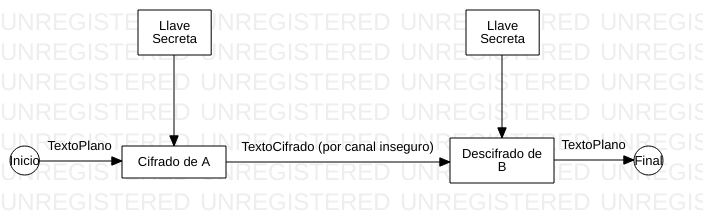
\includegraphics[width=14cm]{./imagenes/MarcoTeorico/cripto_simetrica.png}
        				\caption{Esquema del protocolo de criptografía simétrica.}
        			\end{center}
        		\end{figure}
        		
        		\subsubsection{Criptografía asimétrica.}
        		En los algoritmos de criptografía asimétrica, el receptor posee una llave pública y una llave privada para poder descifrar los mensajes. Por lo que las llaves tanto publica como privada son diferentes, y como sus nombres lo dicen, la llave publica puede ser mostrada a cualquier usuario y la llave privada sólo puede tenerla el usuario propietario del par de llaves. Por lo tanto, podemos llamar llave de cifrado a la llave publica y llave de descifrado a la llave privada. Algunos de los algoritmos más famosos de criptografía asimétrica son: RSA y ElGamal. \cite{refChaffing}\\
        		En el siguiente esquema se muestran los pasos que sigue un protocolo de criptografía simétrica. Definamos 'A' como una entidad que desea enviar información a otra llamada 'B'. Luego entonces, 'B' enviará a 'A' su llave pública para que 'A' cifre la información utilizandola. Cuando la información (TextoCifrado) haya viajado a través del canal inseguro para que 'B' la reciba, 'B' decifrará el TextoCifrado con su llave privada.
        		
        		\begin{figure}[H]
        			\begin{center}	                  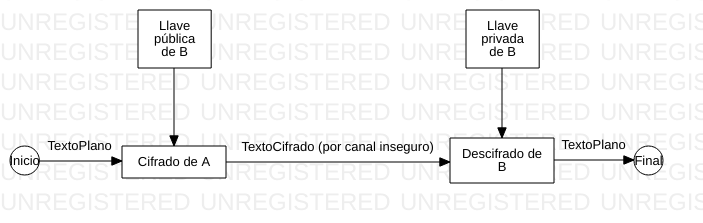
\includegraphics[width=14cm]{./imagenes/MarcoTeorico/cripto_asimetrica.png}
        				\caption{Esquema del protocolo de criptografía asimétrica.}
        			\end{center}
        		\end{figure}
        		
	    
	    %   %   %   %   %   %   %   %   %   
		%		                        %
		%               C&W             %
		%                               %
	    %   %   %   %   %   %   %   %   %
	    \section{Chaffing and Winnowing.}
	    
	    \subsection{Historia}
	    
	    \paragraph{}
	    Chaffing and Winnowing es una t\'ecnica criptogr\'afica que logra confidencialidad sin usar ning\'un proceso de cifrado para el env\'io de datos sobre un canal inseguro. El nombre \textbf{Chaffing and Winnowing} el nombre proviene de la agricultura: D\'espues de que el grano ha sido cosechado y trillado, el grano es mezclado con paja fibrosa no comestible. La paja y el grano son separados por el movimiento de las hojas y la paja es descartada.
	    \'Esta t\'ecnica fue creada por Ron Rivest y fue publicada en un articulo en l\'inea el 18 de Marzo de 1998. \cite{refRivestMIT}
	    A\'unque parece ser similar a un cifrado tradicional y esteganograf\'ia, chaffing and winnowing no puede ser clasificado como uno de ellos.\\
	    \'Esta t\'ecnica permite el env\'io de datos evitando la responsabilidad del cifrado de su contenido. Cuando se usa chaffing and winnowing, el emisor transmite el mensaje sin cifrar (texto plano). Aunque el emisor y el receptor comparten una llave, ellos la usan s\'olo para autentificar. Sin embargo, una tercera parte puede hacer su comunicaci\'on confidencial durante el env\'io simult\'aneo de mensajes especialmente mensajes diseñados a traves del mismo canal.
	    
	    \subsection{¿Qu\'e es Chaffing and Winnowing?}
	    
	    \paragraph{}
	        Chaffing and Winnowing es un nuevo esquema establecido por Rivest en 1998. Este esquema ofrece confidencialidad para el contenido de un mensaje sin involucrarse con cifrado ni estenografía. \cite{refChaffing}
	    
        El proceso \textbf{Chaffing} no hace uso de un cifrado por lo que no tiene una ''clave de cifrado''. Este proceso consiste en agregar paquetes inv\'alidos (Informaci\'on innecesaria) al mensaje a enviar, haciendo que el mensaje viaje seguro a la vista de todos los posibles ''atacantes''.\\
        El proceso de \textbf{Winnowing} no emplea alg\'un tipo de cifrado, por lo que al igual que el proceso chaff no tiene una ''clave de descifrado''. Intentando regular la confidencialidad que provee un cifrado damos paso a la esteganograf\'ia y el proceso de winnowing.\cite{refRivestMIT}
        
        \paragraph{}
        Existen dos partes en el envio de mensajes con winnowing: Autentificaci\'on (Agregando MACs) y agregando paquetes chaff. Nosotros nos enfocaremos mas al uso de paquetes chaff para el env\'io seguro de informaci\'on, ya que, el receptor es quien remueve los paquetes chaff para obtener el mensaje original. 
        
        \paragraph{}
        Los siguientes esquemas explican como es que se lleva a cabo el proceso de \textbf{Chaffing and Winnowing} en diferentes escenarios.
        
		\paragraph{}
		\textbf{Escenario 1:} Alice se est\'a comunicando con Bob en un solo camino de comunicación sobre un canal inseguro y Charles agrega los paquetes de Chaff.\\
		\begin{figure}[!htb]
			\begin{center}	                  \includegraphics[width=14cm]{./imagenes/MarcoTeorico/chaffProcess.png}
				\caption{Charles agrega los paquetes inválidos.}
			\end{center}
		\end{figure}
		
		En el escenario anterior Alice y Bob se están comunicando mutuamente por un canal de comunicación no seguro, en donde son enviados paquetes no cifrados. Alice y Bob comparten la llave de autentificación la cual será usada para el proceso de autentificación. Cuando Alice envía un mensaje a Bob, su mensaje es autenticado de su lado y es enviado a Charles antes de ser enviado a Bob. Charles agrega los paquetes chaff a la secuencia transmitida por Alice, al agregar los paquetes chaff, Charles provee confidencialidad para la comunicación entre Alice y Bob. Pero donde Charles no conoce la llave secreta compartida entre Alice y Bob. Por lo que el proceso de chaffing no necesita ningún conocimiento de la llave secreta de autentificación compartida.
		\paragraph{}
		\textbf{Escenario 2:} Alice se comunica con Bob en un camino de comunicación inseguro y en el cual Charles no agrega los paquetes chaff si no que multiplexa los flujos de las otras dos partes (David y Elaine). Este escenario es diferente al anterior, ya que se multiplexo el flujo de datos de Alice y Bob con el flujo de datos de David y Jane, y cuando el paquete llega a Bob el flujo de paquetes de David hacia Jane es el chaff de Bob y es descartado y vice versa para Jane.
		
		\begin{figure}[H]
			\begin{center}	                  \includegraphics[width=14cm]{./imagenes/MarcoTeorico/escenario2.png}
				\caption{Charles no agrega los paquetes pero multiplexa los flujos.}
			\end{center}
		\end{figure}
		
		\paragraph{}
		\textbf{Escenario 3:} Alicia se comunica con Bob en un canal de comunicación inseguro y Alice no agrega los paquetes chaff. En este escenario, Alice desarrolla la autentificación de sus mensajes, por lo que Alice aplica chaffing para autentificar los mensajes y producir una secuencia de paquetes que serán transmitidos a Bob por la vía de Charles. Bob lleva a cabo el proceso de winnowing para recuperar el mensaje original.
		
		\subsection{Objetivo de Chaffing and Winnowing}
		
		\paragraph{}
		El objetivo de seguridad del esquema de chaffing-and-winnowing es proporcionar privacidad en un entorno simétrico. 
        Desde un punto de vista de seguridad, este esquema debe tratarse simplemente como un esquema de cifrado simétrico. Hay algunos procesos de ''cifrado'' que toman un mensaje y crean un ''texto cifrado'', y algún proceso de ''descifrado'' toma el texto cifrado y recupera el mensaje, ambos operando bajo una clave secreta en com\'un. (Para el esquema Chaffing and Winnowing es la clave para el MAC). Estos procesos no se implementan de manera ''habitual'', pero, de manera abstracta, deben existir, de lo contrario no se logra la privacidad.  \cite{refRivestSeguridad} \cite{refEncontrarLuegoAdivinar}  
        \begin{center}
            \textit{''No es una propiedad de seguridad novedosa, sino un conjunto novedoso de restricciones en los procesos dirigidos a lograr una propiedad de seguridad estándar''\\
            ''Encontrar-luego-adivinar''. Extensión más directa al caso simétrico de la noción de indistinguibilidad.}
        \end{center}
		
		Haciendo uso de \textbf{Chaffing and Winnowing} se asegura que los adversarios no obtengan información del mensaje transmitido a lo largo de un canal de comunicación inseguro entre dos partes. \\
		Rivest propone un esquema, el cual cuenta con tres partes principales. \cite{refChaffing}
		\begin{enumerate}
		    \item \textbf{Autentificación} Es el proceso de descomponer el mensaje original en un paquete más pequeño y complementar cada paquete con un código de autentificación de mensaje (MAC).
		    \item \textbf{Chaffing} Es el proceso de agregar paquetes inválidos (Chaff packets).
		    \item \textbf{Winnowing} Es el proceso de remover paquetes Chaff para obtener el mensaje original en texto plano.
		\end{enumerate}
		
		\subsection{¿Cómo funciona?}
		
		\paragraph{}
		El esquema de Chaffing and Winnowing deja que cada paquete conste de: 
		\begin{itemize}
		    \item Un número de serie
		    \item Contenido del paquete
		    \item Código de autentificación del mensaje
		\end{itemize}
		Cuando son enviados los paquetes, el mensaje con el texto plano se descompone en pequeños paquetes los cuales contienen datos y el tamaño del paquete original. Entonces, el emisor (Alice) usa el algoritmo de \textbf{código de autentificación de mensaje} (MAC) para generar el valor MAC para ser agregado al paquete y el cual se basa en el número de serie, contenido del paquete y la llave autentificación. A continuación se muestra la salida del paquete después del proceso de autentificaci\'on.
		\begin{figure}[H]
			\begin{center}	                  \includegraphics[width=7cm]{./imagenes/MarcoTeorico/descomposicionChaffing.png}
				\caption{Secuencia de Chaffing después del proceso de autentificación.}
			\end{center}
		\end{figure}
		Esta secuencia de paquetes es enviada a Charles (ISP) para llevar a cabo el proceso de Chaffing. Charles agrega paquetes chaff a la secuencia de paquetes antes de ser enviados por medio del canal de comunicación y ser recibidos por Bob. \\
		Existen dos maneras donde Charles puede enviar la secuencia de chaff hacia Bob. La primera es enviando aleatoriamente mezclados los paquetes chaff para formar una secuencia y la otra manera es enviarlos de manera ordenada por el n\'umero de serie seguido del contenido del mensaje. En la siguiente figura se muestra cómo es el proceso de chaff en esta secuencia.
		\begin{figure}[H]
         \centering
          \subfloat[Primera manera]{
           \label{f:Primera manera}
            \includegraphics[width=0.5\textwidth]{./imagenes/MarcoTeorico/firstway_Chaff.png}}
          \subfloat[Segunda manera]{
           \label{f:Segunda manera}
            \includegraphics[width=0.5\textwidth]{./imagenes/MarcoTeorico/secondway_Chaff.png}}
         \caption{Las dos maneras para el proceso de chaff pueden ser utilizadas. Los paquetes chaff son los mensajes de color rojo.}
         \label{f:Enfoques}
        \end{figure}
		Una vez que la secuencia de chaff llega a Bob, el último proceso es Winnowing. Bob determina la secuencia del mensaje que es válida del paquete chaff usando una función hash para el contenido de cada paquete y la llave de autentificación para re-calcular el MAC y compararlo contra el MAC del paquete recibido, si la comparación falla, el paquete chaff es descartado. Si la comparaci\'on es valida, entonces el paquete es parte del mensaje original. La siguiente imagen muestra el proceso completo de chaffing and winnowing.
		\begin{figure}[H]
			\begin{center}	                  \includegraphics[width=14cm]{./imagenes/MarcoTeorico/chaff_winn.png}
				\caption{Visión general del proceso Chaffing and Winnowing.}
			\end{center}
		\end{figure}
        
        \subsection{Propiedades de Chaffing and Winnowing}
        
        \paragraph{}
        \begin{itemize}
		    \item La técnica de Chaffing y Winnowing no depende de la fuerza del esquema de cifrado para proporcionar confidencialidad debido al hecho de que es muy difícil distinguir la informaci\'on \'util de los paquetes chaff sin la clave secreta. Por lo tanto, la dificultad de distinguir la informaci\'on \'util del chaff proporciona confidencialidad al esquema.
		    \item La operación de Chaffing puede ser realizada por un tercero, ya que la clave secreta compartida no es necesaria en el proceso del mismo.
		    \item Los paquetes de Chaff no tienen que contener datos aleatorios, ya que uno podría usar un mensaje válido con una clave secreta diferente para hacer el paquete de Chaff. Cuando el receptor recibe esos paquetes de Chaff, se verán como paquetes de Chaff, ya que la clave que se usa para volver a calcular el Chaff es diferente de la que los hace.
		\end{itemize}
		
		\subsection{All-or-Nothing and the Package Transform (AONT)}
        
        All-or-Nothing and the Package Transform es una variación dentro de la tecnica Chaffing and Winnowing, donde se mejora la eficiencia de su esquema original. AONT es la transformación de pre-procesamiento que permite a las partes enviar más datos (en términos de bit) por paquete en lugar de solo uno. Este pre-procesamiento es una transformación sin cifrado que toma el mensaje de texto sin formato y produce un mensaje empaquetado que luego se procesa de la manera normal de Chaffing and Winnowing. Las definiciones de la transformación AONT son las siguientes:
        
        \begin{enumerate}
            \item El algoritmo de transformación es \textbf{reversible}: Dado el bloque de mensaje transformado, el receptor puede obtener el mensaje de texto sin formato original.
            \item El algoritmo de transformación y su inverso son \textbf{computables} de manera eficiente: Lo que significa que es computacionalmente factible recrear el texto original dada la llave privada y recibir todos los paquetes con éxito.
            \item La transformación no es \textbf{computacionalmente factible}: Esto significa que si se ha recibido parte del paquete de la transmisión, cualquiera que esté intentando leer el mensaje no puede hacerlo ya que la transformación \textbf{AONT} requiere que se reciba todo el mensaje, de lo contrario no entrega nada.
            \item La transformación es una \textbf{técnica sin cifrado}: La técnica de pre-procesamiento no tiene llaves y no hay una llave secreta compartida involucrada en la operación. Cualquier persona que haya recibido todos los mensajes transformados del paquete puede recuperar el mensaje de texto original.
        \end{enumerate}
        
        \paragraph{}
        \textbf{¿Cómo funciona AONT?}
        
        \paragraph{}
        Supongamos que el mensaje de entrada es el siguiente: $m_{1},m_{2},...,m_{n}$.\\
        Seleccionamos una llave aleatoria $K'$ el cual se usará para la función del paquete de transformación.\\
        Se calcula la secuencia transformada ${m'}_{1}, {m'}_{2},...,{m'}_{s}$ para ${s'}=s+1$ como se muestra a continuación:\\
        Tenemos:
        \begin{center}
            $m_{i} \otimes E(K',i)$ for  $i=1,2,3,...,s$
        \end{center}
        También:
        \begin{center}
            $m'_{s'}=K' \otimes h_{1} \otimes h_{2} \otimes ... \otimes h_{s}$
        \end{center}
        
        Donde:
        \begin{center}
            $h_i=E(K_0,m'_i \otimes i)$ for $i=1,2,...,s$
        \end{center}
        
        Donde $K_0$ es una llave conocida pública fija.\\
        Para que el receptor en el otro extremo obtenga el $K_0$, el cual es la llave para el uso de \textbf{AONT}, el receptor realiza el siguiente cálculo:
        
        \begin{center}
            $K'=m'_s \otimes h_1 \otimes h_2 \otimes ... \otimes h_s$
        \end{center}
        \begin{center}
            $m_i=m'_i \otimes E(K',i)$ for $i=1,2,...,s$
        \end{center}
        
        \paragraph{}
        AONT toma el mensaje de texto sin formato de entrada y los transforma, luego crea un bloque para almacenar los mensajes transformados antes de pasar al proceso de autentificación. Después, se genera el paquete Chaff (la cantidad de paquetes Chaff no tiene que ser igual a los paquetes de la informaci\'on \'util).\\
        Esta técnica produce una menor sobrecarga que la sugerencia número 1. El AONT ofrece más confidencialidad al esquema de Chaffing and Winnowing, ya que el adversario debe recibir todo el bloque de mensajes de transformación e identificar correctamente todo el paquete de la informaci\'on \'util para obtener el mensaje de texto original. La siguiente figura muestra la
        descripción general de Chaffing y Winnowing si se agrega la función AONT.
        
        \begin{figure}[H]
			\begin{center}	          \includegraphics[width=14cm]{./imagenes/MarcoTeorico/chaffVsCrypto.png}
				\caption{Proceso de Chaffing and Winnowing junto con AONT.}
			\end{center}
		\end{figure}
        
        \paragraph{}
        \textbf{¿Cómo AONT puede hacer la diferencia?}\\
        
        \begin{enumerate}
            \item Requiere menos ancho de banda al transferir paquetes, ya que se pueden transferir más bits en un paquete en lugar de un bit por paquete.
            \item Los paquetes Chaff son más fáciles de generar, ya que AONT transforma el mensaje de texto plano en bits aleatorios.
            \item La distinción entre Chaffing and Winnowing es más difícil: Si el adversario va a ejercer fuerza bruta en los paquetes, la tarea se ralentizará por el factor del número de bloque de mensajes. Dado que el bloque de mensaje de información adicional se mezcla aleatoriamente dentro de los flujos de paquetes de Chaffing and Winnowing, sin saber que es muy difícil que el bloque adicional proporcione la posibilidad de elegir el bloque de mensaje correcto de los paquetes para obtener el texto plano original.
        \end{enumerate}
        
        \subsection{Comparando Chaffing and Winnowing contra Cifrado y Esteganograf\'ia}
        
        En esta sección explicaremos porque Chaffing and Winnowing no puede ser clasificado como una técnica de cifrado o Estenografía.\\
        
        \subsubsection{Chafing and Winnowing vs Cifrado}
        
        Nosotros podríamos clasificar Chaffing and Winnowing como un método de cifrado, pero volvamos a recordar el principio de un Cifrado.
        El principal objetivo de un cifrado es ocultar el mensaje en texto plano de tal manera que oculta su contenido con el uso de una clave de cifrado para el texto cifrado.
        Por otro lado, en el esquema original de Chaffing and Winnowing, una llave compartida es usada con el fin de autentificar la validación de los paquetes ya sea del emisor o del receptor. Además, Chaffing and Winnowing no hace uso de ninguna técnica de cifrado para ocultar el contenido de un mensaje y que nadie pueda ver dicho mensaje, solo aquellos con la llave correspondiente pueden determinar que paquetes contienen la información valida. A continuación, se muestra como se puede ver el esquema Chaffing and Winnowing como una técnica de cifrado. 
        
        \begin{figure}[H]
			\begin{center}	                  \includegraphics[width=14cm]{./imagenes/MarcoTeorico/chaffVsCrypto.png}
				\caption{Visualizando el método Chaffing and Winnowing cómo un esquema de cifrado.}
			\end{center}
		\end{figure}
        
        Chaffing y Winnowing pueden verse como \textbf{un tipo especial de esquema de cifrado simétrico}, ya que la operación \textbf{chaffing} es similar al ''proceso de cifrado''. En la operación de chaffing, el texto cifrado se crea para producir un paquete de la informaci\'on \'util no válido que se envía al receptor. Luego, el receptor realiza el ''proceso de descifrado'', que implica descartar el paquete de desperdicios y recuperar el mensaje original. Ambas operaciones operan bajo una llave secreta común que se usa para derivar el valor MAC.\\
        
        Pero la diferencia es, \textit{Chaffing y Winnowing} dos partes que no buscan lograr la confidencialidad. El emisor comparte una clave secreta con el receptor para que el receptor pueda usar la clave secreta para autentificarse (si se afirma que el mensaje recibido proviene del remitente deseado). Pero la ganancia de confidencialidad proviene de la dificultad de distinguir el paquete Chaff del paquete de la informaci\'on \'util. Mientras que en el cifrado, la clave se utiliza para lograr la confidencialidad mediante la creación de texto cifrado que oculta el contenido del mensaje de personas.
        
        Chaffing y Winnowing junto con el esquema AONT, el esquema en sí es muy parecido al cifrado, excepto que la clave que se usa en la transformación AONT se elige aleatoriamente cada vez en lugar de fijarla. Además, el último bloque de mensajes es exclusivo o de la clave y todo el hash del bloque de mensajes está allí para garantizar que cualquier modificación en el bloque de mensajes cambiará la clave $K'$ calculado por el receptor. Por lo tanto, el último bloque de mensajes ${m'}_{s'}$ está allí solo con el propósito de autentificación. Por lo tanto, Chaffing y Winnowing con el esquema AONT no pueden ser clasificados bajo cifrado.\\
        
        \subsubsection{Chaffing and Winnowing vs Esteganograf\'ia}
        
        Para algunas personas, Chaffing and Winnowing puede ser clasificado como una técnica esteganograf\'ia. Sin embargo, el objetivo principal de la estenografía es el de ocultar el mensaje original dentro de otro tipo de mensaje, por lo tanto, nadie aparte del emisor y el receptor sabrá que hay un mensaje oculto. Contrario a Chaffing and Winnowing, en donde cualquiera puede ver el contenido del mensaje, ya que este método no trata de esconderlo de los posibles atacantes.\\
        Otra diferencia es que en esteganograf\'ia el emisor tiene que ocultar el mensaje el mismo, mientras que en Chaffing and Winnowing no necesariamente es así, ya que una ''tercera parte'' puede hacerlo.\\
        Por lo tanto, Chaffing and Winnowing no puede ser considerado como esteganograf\'ia.\\
        
    \begin{comment}
	    \section{Extensiones de Google Chrome.}
		Como hemos mencionado antes, realizaremos una extensión de Google Chrome, por lo que empezaremos  explicando que son estas extensiones. Una extensión de Google Chrome es una pequeña aplicación que se instala en el navegador que, en cierta medida, mejora la navegación del usuario. Estas extensiones tienen diferentes funcionalidades, las cuales mejoran la experiencia del usuario durante su navegación por la internet.\\
		Existen muchas extensiones hoy en día con funcionalidades variadas para distintos usos para los servicios web. La instalación de las extensiones es una tarea fácil gracias a Chrome Web Store. Chrome Web Store es una tienda en línea de aplicaciones web para el navegador Google Chrome, y la cual es desarrollada y mantenida por Google. Esta tienda es más intuitiva y amigable para cualquier usuario, facilitando la instalación de las extensiones con un simple ''click''.\\
		
		\section{Seguridad en internet.}
		En la actualidad, el incremento constante de internet ha impactado directamente en la seguridad de la información que se maneja cotidianamente y por la mayoría de usuarios. Existen infinidad de sitios donde es aplicada la seguridad, ya que sin ésta, se verían afectados todos los usuarios en  sus cuentas, pudiendo verse afectados desde un posible \Gls{Robo de Identidad} (Robo de identidad), hasta la perdida de dinero real dado que la base de algunas de éstas paginas son E-Commerce, estas paginas implican el manejo de tarjetas de crédito, paypal, etc.\\
		
		Uno de los puntos más críticos de la seguridad en Internet son las herramientas que interactúan de forma directa con los usuarios. Es común escuchar sobre fallas en los sistemas de protección de los servidores más frecuentemente utilizados, por ejemplo Apache, NGINX, IIS, etc. O en los lenguajes de programación en que son escritas las aplicaciones. \cite{refSeguridadWeb} Sin embargo, la vulnerabilidad más grande dentro de un sistema, son los ataques directos a los usuarios finales durante la autentificación.\\
		
		\section{Cookies.}
		Durante la navegación por internet, la información sobre la computadora puede ser colectada y almacenada. Ésta puede ser de carácter general sobre el equipo y puede ser también información más específica sobre los hábitos de navegación del usuario, toda esta información guardada se le conoce como \Gls{cookies}\cite{refCookies}. \\
		A continuación se muestran los diferentes tipos de cookies que existen para los navegadores.
		
		\begin{itemize}
		    \item \textbf{Cookies propias:} Las cookies se gestionan desde el terminal o dominio de un mismo editor.
		    \item \textbf{Cookies de terceros:} Las cookies no son enviadas por el propio editor, sino por otra entidad.  
		    \item \textbf{Cookies de sesión:} Los datos recabados sólo se recogen mientras el usuario está navegando por la página web.
		    \item \textbf{Cookies persistentes:} Los datos continúan almacenados en el terminal y se puede acceder a ellos durante un periodo de tiempo determinados.
		    \item \textbf{Cookies técnicas:} Permiten controlar el tráfico y la comunicación de datos.		
            \item \textbf{Cookies de personalización:} Dejan a los usuarios acceder según algunas características propias que se recogen (navegador, idioma, etc.).
            \item \textbf{Cookies de análisis:} Recogen datos sobre el comportamiento de los usuarios y permiten elaborar un perfil de usuario.
            \item \textbf{Cookies publicitarias:} Recogen datos sobre la gestión de los espacios publicitarios.
        \end{itemize}
		
		Las cookies persistentes son aquellas que se almacenan en el equipo para que las preferencias personales puedan ser retenidas, ayudan a los sitios web a recordar tu información y ajustes cuando los visitas más adelante. Esto conlleva un acceso más rápido y sencillo ya que, por ejemplo, no se tiene que iniciar sesión de nuevo. Además de la autentificación, otras páginas web tienen más funciones para las cookies permanentes, como: selección de idioma, selección de tema, preferencias de menú, marca-páginas internos de la web, o favoritos. \cite{refCookiesPersistentes}
		Muchos navegadores pueden ajustar el periodo de tiempo en que las cookies persistentes deben ser almacenadas. \\
		Gracias a las cookies persistentes, las direcciones de correo electrónico aparecen por default cuando se abre el correo electrónico, o en páginas de inicio personalizadas cuando se visita en línea un comercio. Si un atacante obtiene acceso puede recopilar información personal del usuario través de estos archivos y poder robar toda información del usuario. Es fácil acceder a estas cookies y obtener fácilmente la información del usuario, por lo que es necesario que el usuario nunca deje vulnerable esta información o en su debido caso borrar cookies al término de cada sesión.
		Existen diferentes funcionalidades para las cookies, una de las más importantes es la funcionalidad de seguridad, ya que contiene información importante de los usuarios. A continuación se muestran las diferentes funcionalidades de las cookies.
		
		\begin{itemize}
		    \item \textbf{Preferencias:} Sirven para que la página se visualice atendiendo a los gustos del usuario, como por ejemplo idioma, región o tamaño de textos.
		    \item \textbf{Seguridad:} Se encargan de autentificar a los usuarios y evitar el uso fraudulento de las credenciales por parte de terceros.
		    \item \textbf{Procesos:} Son utilizadas para el correcto funcionamiento de la página en el navegador.
		    \item \textbf{Publicitarias/Estadísticas:} Se usan para que la publicidad que se muestre sea personalizada.
		    \item \textbf{Estados de la sesión:} Obtienen información del comportamiento del usuario en una página web, como por ejemplo el tiempo que pasa en una página, los çlicks”que realiza o la publicidad que le aparece.
		\end{itemize}
		
		Las cookies pueden ayudar al usuario en varios aspectos durante su navegación, gracias a sus distintas funcionalidades, pero a la vez son muy vulnerables, ya que la información no se encuentra cifrada, haciendo que cualquier tercero pueda ver esa información. A continuación presentamos los distintos problemas que se pueden presentar al hacer uso de las cookies.
		
		\begin{itemize}
		    \item \textbf{Software del equipo o en el navegador web:} Los fallos que tiene el software o las vulnerabilidades de los protocolos que utiliza el navegador, pueden permitir que se puedan robar las cookies de sesión (credenciales).
		    \item \textbf{Tiendas online fraudulentas:} Las cookies de terceros registran todas las búsquedas que realizamos, por ejemplo, de productos y servicios. El fraude se produce cuando, usando estos datos almacenados en las cookies, el usuario es redirigido hacia tiendas fraudulentas, mediante publicidad engañosa que le muestra precios muy bajos de artículos o servicios de los que previamente ha realizado búsquedas.
		    \item \textbf{Noticias falsas o fake news:} Es una variante de la anterior pero orientada a la visualización de artículos de videos de carácter sesgado o sensacionalista que incitan al usuario a acceder a una página web o ver un video.
		    \item \textbf{Robo de cookies o secuestro de sesión:} Se introduce una cookie modificada en el navegador del usuario que previamente ha accedido a una web controlada por los ciber-delincuentes. Cuando accede a una página que requiere autentificación la cookie modificada se hace pasar por la cookie legítima, obteniendo las credenciales del usuario, por ejemplo, de su correo electrónico o redes sociales.
		\end{itemize}
	
		Antes de comenzar por explicar los sistemas criptográficos a usar, es necesario identificar algunos objetivos de seguridad de la información los cuales se explican en el cuadro 4. \cite{refCryptography}\\
		
		\begin{table}[H]
		\centering
		\resizebox{14cm}{!} {
            \begin{tabular}{|l|l|l}
            \cline{1-2}
            Objetivo            & Descripción                                                                                                                                                  &  \\ \cline{1-2}
            Confidencialidad    & \begin{tabular}[c]{@{}l@{}}Mantiene secreta la información para \\ todos los usuarios pero solo a aquellos \\ que están autorizados pueden verla.\end{tabular} &  \\ \cline{1-2}
            Integridad de datos & \begin{tabular}[c]{@{}l@{}}Asegura que la información no haya sido \\ alterada por un usuario no autorizado.\end{tabular}                                       &  \\ \cline{1-2}
            Identificación      & Corrobora la identidad de una entidad.                                                                                                                        &  \\ \cline{1-2}
            Autentificación     & Corrobora la fuente de información.                                                                                                                           &  \\ \cline{1-2}
            Firma               & \begin{tabular}[c]{@{}l@{}}Es un medio para vincular la información \\ de la entidad.\end{tabular}                                                            &  \\ \cline{1-2}
            Autorización        & \begin{tabular}[c]{@{}l@{}}Transferencia, hacia otra entidad, de la \\ sanción oficial para hacer o no hacer algo.\end{tabular}                               &  \\ \cline{1-2}
            Validación          & \begin{tabular}[c]{@{}l@{}}Un medio para proporcionar la oportunidad \\ de uso o manipular información o recursos.\end{tabular}                               &  \\ \cline{1-2}
            Certificación       & Aval de información por una entidad de confianza.                                                                                                            &  \\ \cline{1-2}
            Tiempo de marcado   & \begin{tabular}[c]{@{}l@{}}Registro de tiempo de creación o existencia \\ de información.\end{tabular}                                                        &  \\ \cline{1-2}
            Recepción           & Reconocimiento de que se ha recibido la información.                                                                                                          &  \\ \cline{1-2}
            Confirmación        & Conocimiento de que se ha prestado servicios.                                                                                                                 &  \\ \cline{1-2}
            Anonimato           & \begin{tabular}[c]{@{}l@{}}Oculta de identidad de una entidad involucrada en \\ algunos procesos.\end{tabular}                                                &  \\ \cline{1-2}
            No repudio          & \begin{tabular}[c]{@{}l@{}}Prevención de la denegación de compromisos o acciones \\ anteriores.\end{tabular}                                                  &  \\ \cline{1-2}
            \end{tabular}
            }
            \caption{Objetivos de la seguridad de la información}
            \end{table}
		
		\section{Concepto de cifrado.}
		El cifrado es el proceso de disfrazar un mensaje de texto plano de tal manera que no es posible leer por cualquier persona excepto aquellas personas que tengan la llave secreta. Un mensaje cifrado es conocido como ''texto cifrado'' (ciphertext). El proceso de convertir este cifrado en texto plano de nuevo se le llama ''descifrado''. 
		%Existen dos maneras generales de cifrado basado en llaves, los cuales son: Algoritmos de cifrado simétrico y Algoritmos de cifrado asimétrico. \cite{refChaffing}\\
	
    	\section{Criptología.}
    	La Criptología (proveniente del griego << kryptos >> que significa ''oculto'' y << logos >> que significa ''tratado'' o ''ciencia'') es la ciencia que trata las escrituras ocultas. Está comprendida por la Criptografía, el Criptoanálisis y la Estenografía. Más adelante en esta sección, se adentrará en la definición de criptografía y estenografía, con el fin de explicar y clasificar a la técnica Chaffing and Winnowing.
    	
        \subsection{Criptografía.}
        La criptografía proviene del griego "kryptos" que significa oculto, y "graphia", que significa escritura, y su definición según el diccionario de la Real Academia de la Lengua Española es: Arte de escribir con clave secreta o de un modo enigmático. La criptografía es un conjunto de técnicas, que originalmente tratan sobre la protección o el ocultamiento de la información frente a observadores no autorizados. Entre las disciplinas que engloba cabe destacar la Teoría de la Información, la Complejidad Algorítmica y la Teoría de números o Matemática Discreta, que como ya sabemos estudia las propiedades de los números enteros.\cite{refCryptography}\\

        A través de la criptografía la información puede ser protegida contra el acceso no autorizado, su modificación y la inserción de información extra. También puede ser usada para prevenir el acceso y uso no autorizado de los recursos de una red o sistema informático y para prevenir a los usuarios la denegación de los servicios a los que sí están permitidos. Modernamente, la criptografía es la metodología para proveer la seguridad de las redes telemáticas, incluyendo la identificación de entidades y autentificación, el control de acceso a los recursos, la confidencialidad de los mensajes transmitidos, la integridad de los mensajes y su no repudio. Existen dos maneras generales de cifrado basado en llaves, los cuales son: Algoritmos de cifrado simétrico y Algoritmos de cifrado asimétrico.\\
        
        Denotemos a $M$ como un mensaje de texto plano o un flujo de datos de bits. Pero para el computador, $M$ es un dato binario y un mensaje a ser cifrado. Denotemos también a $C$ como un texto cifrado, el cual, puede ser de tamaño corto o tan largo como $M$, dependiendo si se combina cifrado y compresión en el mismo proceso. La función de cifrado $E$ opera en $M$ para producir $C$.
		
		\begin{center}
		    $E_{k}(M) = C$    
		\end{center}
		
		Para el proceso de descifrado, se ocupa la función $D$, la cual opera en $C$ para recuperar el mensaje $M$.
		
		\begin{center}
		    $D_{k}(C) = M$
		\end{center}
		
		Por lo tanto, podemos decir que tanto el proceso de cifrado y descifrado nos provee la misma entrada y la misma salida, respectivamente, donde ésta es el mensaje original. Por lo que la siguiente identidad es trivial.
		
		\begin{center}
		    $D_{k}(E_{k}(M)) = M$
		\end{center}
        \cite{refChaffing}
		\subsubsection{Criptografía simétrica.\\}
	    En la criptografía simétrica, tanto el emisor como el receptor comparten una única llave secreta para cifrar y descifrar la información que se deseé transmitir. Esto implica que ambas partes de la comunicación deben tener un acuerdo antes de que se realice la comunicación. La seguridad de este tipo de algoritmos radica en mantener segura la llave secreta, por tanto, si ésta es revelada, cualquiera con acceso a ella puede descifrar el mensaje. Por estas razones, este tipo de criptografía puede ser visto como ''criptografía de llave privada''. \cite{refChaffing}
		\subsubsection{Criptografía asimétrica.\\}
		En los algoritmos para criptografía asimétrica, el receptor posee una llave pública y una llave privada para poder descifrar los mensajes. Por lo que las llaves tanto publica como privada son diferentes, y como sus nombres lo dicen, la llave publica puede ser mostrada a cualquier usuario y la llave privada sólo puede tenerla el usuario propietario del par de llaves.\\
		Por lo tanto, podemos llamar llave de cifrado a la llave publica y llave de descifrado a la llave privada.
		Para evitar confusión con criptografía simétrica y asimétrica, el proceso de cifrado y descifrado pueden ser denotados como lo mismo. Dado que, uno puede usar el cifrado de clave pública para evitar la pérdida de una clave, pero facilita el control. (Con criptografía asimétrica, el emisor y receptor deben compartir una llave y este proceso puede ser complicado). Lo anterior es explicado con un ejemplo, donde la llave de cifrado y descifrado son diferentes.\cite{refChaffing}\\
		
		%Poner arriba cuando se habla en criptografía en general de aqui hasta el diagrama antes de Estenografía???
		
		
		Entonces, decimos que para la criptografía asimétrica existe un par de llaves (publica y privada), por tanto las funciones puedes describirse como:
		
		\begin{center}
		$E_{k_{1}}(M) = C$
		\\
		$D_{k_{2}}(C) = M$
		\end{center}
		
		Por tanto.
		
		\begin{center}
		    $D_{k_{2}}(E_{k_{1}}(M)) = M$
		\end{center}
		
		\paragraph{}
		Este proceso se puede visualizar más fácilmente con el siguiente diagrama.
		
		\begin{figure}[!htb]
			\begin{center}	        	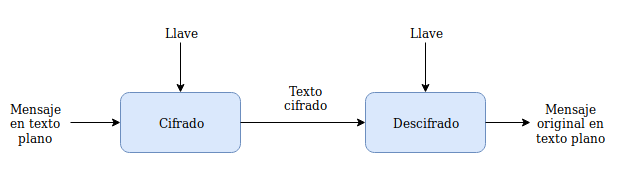
\includegraphics[width=14cm]{./imagenes/cifrado.png}
				\caption{Proceso de cifrado y descifrado.}
			\end{center}
		\end{figure}
	
		%Estenografía
		\subsection{Esteganografía.}
		
		La esteganograf\'ia es una t\'ecnica en la criptograf\'ia, la cual tiene como objetivo lograr la confidencialidad sin ningún proceso de cifrado. Es una manera de esconder un mensaje secreto tal que la existencia del mensaje escondido sea imposible de detectar. Esto involucra esconder un mensaje oculto en algún tipo de archivo digital, el cual contiene bits redundantes donde poder esconder el mensaje, tal que altera los bits más insignificantes de cada byte del archivo digital con los bits del mensaje secreto.\\
		
		Como resultado de esto, la \textbf{NSA} y \textbf{FBI} declararon 2 formas que permiten al gobierno controlar la criptografía en Estados Unidos:
        \begin{enumerate}
            \item \textbf{Propuesta clave de depósito de garantía} (KEP): Esta propuesta requiere que el usuario se registre en su software de cifrado de llave con el gobierno.
            \item \textbf{Propuesta de Recuperacion de Clave} (KRP): Esta propuesta provee el permiso para el gobierno de tener acceso al ''\Gls{backdoor}'' para obtener la llave de acceso para descifrar el mensaje cifrado
        \end{enumerate}
		
		\section{Chaffing and Winnowing.}
		
		Chaffing and Winnowing es un nuevo esquema establecido por Rivest en 1998. Este esquema ofrece confidencialidad para el contenido de un mensaje sin involucrarse con cifrado ni estenografía, sin embargo, ofrece los cuatro objetivos principales de la Criptografía, los cuales son:
		\begin{enumerate}
			\item \textbf{Confidencialidad} Mantiene la información secreta para todos los usuarios excepto para los usuarios que estén autorizados para visualizarlos u obtenerlo.
			\item \textbf{Integridad de datos} Asegura que la información no haya sido alterada por medios no autorizados o desconocidos.
			\item \textbf{autentificación} Confirma la identidad de una entidad.
			\item \textbf{No repudio} Previene la denegación de compromisos o acciones anteriores.
		\end{enumerate}

		El objetivo de \textbf{Chaffing and Winnowing} es asegurar que los adversarios no obtengan información del mensaje transmitido a lo largo de un canal de comunicación inseguro entre dos partes. El esquema de Rivest consiste en tres partes principales.
		\begin{enumerate}
		    \item \textbf{Autentificación} Es el proceso de descomponer el mensaje original en un paquete más pequeño y complementar cada paquete con un código de autentificación de mensaje (MAC).
		    \item \textbf{Chaffing} Es el proceso de agregar paquetes inválidos (Chaff packets).
		    \item \textbf{Winnowing} Es el proceso de remover paquetes Chaff para obtener el mensaje original en texto plano.
		\end{enumerate}
		
		El la figura 2, se muestra el paso ''Chaffing'', la cual muestra donde se agregan los paquetes inválidos (Chaff packets).
		\paragraph{}
		\textbf{Escenario 1:} Alice esta comunicando con Bob en un solo camino de comunicación sobre un canal inseguro y Charles (Proveedor de servicios de Internet) agrega los paquetes de Chaff.\\
		\begin{figure}[!htb]
			\begin{center}	                  \includegraphics[width=14cm]{./imagenes/chaffProcess.png}
				\caption{Charles agrega los paquetes inválidos.}
			\end{center}
		\end{figure}
		
		En el escenario anterior Alice y Bob se están comunicando mutuamente por un canal de comunicación no seguro, en donde son enviados paquetes no cifrados. Alice y Bob comparten la llave de autentificación la cual será usada para el proceso de autentificación. Cuando Alice envía un mensaje a Bob, su mensaje es autenticado de su lado y es enviado a Charles antes de ser enviado a Bob. Charles agrega los paquetes chaff a la secuencia transmitida por Alice, al agregar los paquetes chaff, Charles provee confidencialidad para la comunicación entre Alice y Bob. Pero donde Charles no conoce la llave secreta compartida entre Alice y Bob. Por lo que el proceso de chaffing no necesita ningún conocimiento de la llave secreta de autentificación compartida.
		\paragraph{}
		\textbf{Escenario 2:} Alice se comunica con Bob en un camino de comunicación inseguro y en el cual Charles no agrega los paquetes chaff si no que multiplexa los flujos de las otras dos partes (David y Elaine). Este escenario es diferente al anterior, ya que se multiplexo el flujo de datos de Alice y Bob con el flujo de datos de David y Jane, y cuando el paquete llega a Bob el flujo de paquetes de David hacia Jane es el chaff de Bob y es descartado y vice versa para Jane.
		
		\begin{figure}[H]
			\begin{center}	                  \includegraphics[width=14cm]{./imagenes/escenario2.png}
				\caption{Charles no agrega los paquetes pero multiplexa los flujos.}
			\end{center}
		\end{figure}
		
		\newpage
		\textbf{Escenario 3:} Alicia se comunica con Bob en un canal de comunicación inseguro y Alice no agrega los paquetes chaff. En este escenario, Alice desarrolla la autentificación de sus mensajes, por lo que Alice aplica chaffing para autentificar los mensajes y producir una secuencia de paquetes que serán transmitidos a Bob por la vía de Charles. Bob lleva a cabo el proceso de winnowing para recuperar el mensaje original.

		\subsection{¿Como funciona Chaffing and Winnowing?}
		
		El esquema de Chaffing and Winnowing deja que cada paquete conste de: un número de serie, contenido del paquete y el código de autentificación del mensaje.
		Cuando son enviados los paquetes, el mensaje con el texto plano se descompone en pequeños paquetes los cuales contienen datos y el tamaño del paquete original. Entonces, el emisor (Alice) usa el algoritmo de \textbf{código de autentificación de mensaje} (MAC) \Gls{HMACSHA14} para generar el valor MAC para ser agregado al paquete y el cual se basa en el número de serie, contenido del paquete y la llave autentificación. A continuación se muestra la salida del paquete después de la autentificación.
		
		\begin{figure}[H]
			\begin{center}	                  \includegraphics[width=8cm]{./imagenes/descomposicionChaffing.png}
				\caption{Secuencia de Chaffing después del proceso de autentificación.}
			\end{center}
		\end{figure}
		
		Esta secuencia de paquetes es enviada a Charles (ISP) para llevar a cabo el proceso de Chaffing. Charles agrega paquetes chaff a la secuencia de paquete    s antes de ser enviados por medio del canal de comunicación y ser recibidos por Bob. Ahora, existen dos maneras donde Charles puede enviar la secuencia de chaff hacia Bob. La primera es enviando aleatoriamente mezclados los paquetes chaff para formar una secuencia y la otra manera es enviarlos de manera ordenada por el n\'umero de serie seguido del contenido del mensaje. En la siguiente figura se muestra cómo es el proceso de chaff en esta secuencia.
		
		\begin{figure}[H]
         \centering
          \subfloat[Primera manera]{
           \label{f:Primera manera}
            \includegraphics[width=0.5\textwidth]{./imagenes/firstway_Chaff.png}}
          \subfloat[Segunda manera]{
           \label{f:Segunda manera}
            \includegraphics[width=0.5\textwidth]{./imagenes/secondway_Chaff.png}}
         \caption{Las dos maneras para el proceso de chaff pueden ser utilizadas. Los paquetes chaff son los mensajes de color rojo.}
         \label{f:Enfoques}
        \end{figure}
		
		Una vez que la secuencia de chaff llega a Bob, el último proceso es Winnowing. Bob determina la secuencia del mensaje que es válida del paquete chaff usando una función hash para el contenido de cada paquete y la llave de autentificación para re-calcular el MAC y compararlo contra el MAC del paquete recibido, si la comparación falla, el paquete chaff es descartado. 
		La siguiente imagen muestra el proceso completo de chaffing and winnowing.
		
		\begin{figure}[H]
			\begin{center}	                  \includegraphics[width=14cm]{./imagenes/chaff_winn.png}
				\caption{Visión general del proceso Chaffing and Winnowing.}
			\end{center}
		\end{figure}
		
		\subsection{Propiedades de Chaffing and Winnowing}
		\begin{itemize}
		    \item La técnica de Chaffing y Winnowing no depende de la fuerza del esquema de cifrado para proporcionar confidencialidad debido al hecho de que es muy difícil distinguir la informaci\'on \'util de los paquetes chaff sin la clave secreta. Por lo tanto, la dificultad de distinguir la informaci\'on \'util del chaff proporciona confidencialidad al esquema.
		    \item La operación de Chaffing puede ser realizada por un tercero, ya que la clave secreta compartida no es necesaria en el proceso del mismo.
		    \item Los paquetes de Chaff no tienen que contener datos aleatorios, ya que uno podría usar un mensaje válido con una clave secreta diferente para hacer el paquete de Chaff. Cuando el receptor recibe esos paquetes de Chaff, se verán como paquetes de Chaff, ya que la clave que se usa para volver a calcular el Chaff es diferente de la que los hace.
		\end{itemize}
        
        \subsection{Enfoques alternativos para el esquema de Chaffing and Winnowing}
        
        Existes dos sugerencias que se pueden utilizar en este esquema. El primero es iniciar los paquetes de la informaci\'on \'util que contienen un solo bit de datos y dejar los paquetes chaff con los bits complementarios. Ambos contienen un numero de serie y un valor hash del contenido del mensaje. Aplicando ésta sugerencia, se le será muy difícil y casi imposible al adversario identificar los paquetes de la informaci\'on \'util de los paquetes chaff. La siguiente figura demuestra como la secuencia chaff funcionaría si se le aplica ésta primer sugerencia.
        
        \begin{figure}[H]
			\begin{center}	          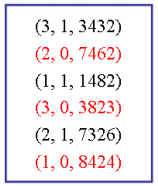
\includegraphics[width=3cm]{./imagenes/esquema1.png}
				\caption{Primer sugerencia, donde los paquetes chaff son de color rojo.}
			\end{center}
		\end{figure}
        
        Claramente, el esquema anterior es muy ineficiente cuando tratamos de enviar mensajes cortos o incluso mensajes largos. Esto puede comprobarse mediante un simple cálculo para mostrar la sobrecarga que se agrega con esta sugerencia.
        
        Supongamos que se utiliza una función hash cuyo valor de hash es de 64 bits de salida y cada paquete contiene un número de serie (1 bit de contenido de datos y el valor de hash del mensaje).
        
        Por lo tanto, tenemos 32 bits, (que es la representación máxima de un valor entero) para el número de serie, 1 bit para el contenido de datos y 64 bits para los valores hash. Entonces, cuando los paquetes ''wheat'' y el paquete chaff se están transmitiendo, tenemos lo siguiente:
        \begin{center}
        $32 + 1 + 64 = 97$
        \end{center}
        El cual es el número total de bits que se transmiten para un solo paquete de la informaci\'on \'util
        \begin{center}
        $32 + 1 + 64 = 97$  
        \end{center}
        El cual es el número total de bits que se transmiten para un solo paquete chaff. Como resultado, este esquema requiere 194 bits para ser transmitido. Aunque esta técnica incremente la seguridad del esquema Chaffing and Winnowing debido a las características adicionales, éste enfoque no es muy eficiente. El valor hash puede ser otro valor como 128, 256, etc. dependiendo del bit de salida de la función hash.\\
        
        La segunda sugerencia es adoptar “All-or-Nothing and Package Transform, (AONT)”.
        Lo que permite muchos bits por paquete y reduce la sobrecarga adicional a cada paquete. 
        Cuando se transfiere un mensaje grande, ésta sugerencia es más eficiente. El detalle de la AONT se tratará en la siguiente sección.\\
        
        \textbf{All-or-Nothing and the Package Transform (AONT)}\\
        
        All-or-Nothing and the Package Transform es una variación dentro de la tecnica Chaffing and Winnowing, donde se mejora la eficiencia de su esquema original. AONT es la transformación de pre-procesamiento que permite a las partes enviar más datos (en términos de bit) por paquete en lugar de solo uno. Este pre-procesamiento es una transformación sin cifrado que toma el mensaje de texto sin formato y produce un mensaje empaquetado que luego se procesa de la manera normal de Chaffing and Winnowing. Las definiciones de la transformación AONT son las siguientes:
        
        \begin{enumerate}
            \item El algoritmo de transformación es \textbf{reversible}: Dado el bloque de mensaje transformado, el receptor puede obtener el mensaje de texto sin formato original.
            \item El algoritmo de transformación y su inverso son \textbf{computables} de manera eficiente: Lo que significa que es computacionalmente factible recrear el texto original dada la llave privada y recibir todos los paquetes con éxito.
            \item La transformación no es \textbf{computacionalmente factible}: Esto significa que si se ha recibido parte del paquete de la transmisión, cualquiera que esté intentando leer el mensaje no puede hacerlo ya que la transformación \textbf{AONT} requiere que se reciba todo el mensaje, de lo contrario no entrega nada.
            \item La transformación es una \textbf{técnica sin cifrado}: La técnica de pre-procesamiento no tiene llaves y no hay una llave secreta compartida involucrada en la operación. Cualquier persona que haya recibido todos los mensajes transformados del paquete puede recuperar el mensaje de texto original.
        \end{enumerate}
        
        \paragraph{}
        \textbf{¿Cómo funciona AONT?}
        
        \paragraph{}
        Supongamos que el mensaje de entrada es el siguiente: $m_{1},m_{2},...,m_{n}$.\\
        Seleccionamos una llave aleatoria $K'$ el cual se usará para la función del paquete de transformación.\\
        Se calcula la secuencia transformada ${m'}_{1}, {m'}_{2},...,{m'}_{s}$ para ${s'}=s+1$ como se muestra a continuación:\\
        Tenemos:
        \begin{center}
            $m_{i} \otimes E(K',i)$ for  $i=1,2,3,...,s$
        \end{center}
        También:
        \begin{center}
            $m'_{s'}=K' \otimes h_{1} \otimes h_{2} \otimes ... \otimes h_{s}$
        \end{center}
        
        Donde:
        \begin{center}
            $h_i=E(K_0,m'_i \otimes i)$ for $i=1,2,...,s$
        \end{center}
        
        Donde $K_0$ es una llave conocida pública fija.\\
        Para que el receptor en el otro extremo obtenga el $K_0$, el cual es la llave para el uso de \textbf{AONT}, el receptor realiza el siguiente cálculo:
        
        \begin{center}
            $K'=m'_s \otimes h_1 \otimes h_2 \otimes ... \otimes h_s$
        \end{center}
        \begin{center}
            $m_i=m'_i \otimes E(K',i)$ for $i=1,2,...,s$
        \end{center}
        
        \paragraph{}
        AONT toma el mensaje de texto sin formato de entrada y los transforma, luego crea un bloque para almacenar los mensajes transformados antes de pasar al proceso de autentificación. Después, se genera el paquete Chaff (la cantidad de paquetes Chaff no tiene que ser igual a los paquetes de la informaci\'on \'util).\\
        Esta técnica produce una menor sobrecarga que la sugerencia número 1. El AONT ofrece más confidencialidad al esquema de Chaffing and Winnowing, ya que el adversario debe recibir todo el bloque de mensajes de transformación e identificar correctamente todo el paquete de la informaci\'on \'util para obtener el mensaje de texto original. La siguiente figura muestra la
        descripción general de Chaffing y Winnowing si se agrega la función AONT.
        
        \begin{figure}[H]
			\begin{center}	          \includegraphics[width=14cm]{./imagenes/chaffVsCrypto.png}
				\caption{Proceso de Chaffing and Winnowing junto con AONT.}
			\end{center}
		\end{figure}
        
        \paragraph{}
        \textbf{¿Cómo AONT puede hacer la diferencia?}\\
        
        \begin{enumerate}
            \item Requiere menos ancho de banda al transferir paquetes, ya que se pueden transferir más bits en un paquete en lugar de un bit por paquete.
            \item Los paquetes Chaff son más fáciles de generar, ya que AONT transforma el mensaje de texto plano en bits aleatorios.
            \item La distinción entre Chaffing and Winnowing es más difícil: Si el adversario va a ejercer fuerza bruta en los paquetes, la tarea se ralentizará por el factor del número de bloque de mensajes. Dado que el bloque de mensaje de información adicional se mezcla aleatoriamente dentro de los flujos de paquetes de Chaffing and Winnowing, sin saber que es muy difícil que el bloque adicional proporcione la posibilidad de elegir el bloque de mensaje correcto de los paquetes para obtener el texto plano original.
        \end{enumerate}
        
        \subsection{Comparando Chaffing and Winnowing contra Cifrado y Estenografía}
        
        En esta sección explicaremos porque Chaffing and Winnowing no puede ser clasificado como una técnica de cifrado o Estenografía.\\
        
        \subsubsection{Chafing and Winnowing vs Cifrado}
        
        Nosotros podríamos clasificar Chaffing and Winnowing como un método de cifrado, pero volvamos a recordar el principio de un Cifrado.
        El principal objetivo de un cifrado es ocultar el mensaje en texto plano de tal manera que oculta su contenido con el uso de una clave de cifrado para el texto cifrado.
        Por otro lado, en el esquema original de Chaffing and Winnowing, una llave compartida es usada con el fin de autentificar la validación de los paquetes ya sea del emisor o del receptor. Además, Chaffing and Winnowing no hace uso de ninguna técnica de cifrado para ocultar el contenido de un mensaje y que nadie pueda ver dicho mensaje, solo aquellos con la llave correspondiente pueden determinar que paquetes contienen la información valida. A continuación, se muestra como se puede ver el esquema Chaffing and Winnowing como una técnica de cifrado. 
        
        \begin{figure}[H]
			\begin{center}	                  \includegraphics[width=14cm]{./imagenes/chaffVsCrypto.png}
				\caption{Visualizando el método Chaffing and Winnowing cómo un esquema de cifrado.}
			\end{center}
		\end{figure}
        
        Chaffing y Winnowing pueden verse como \textbf{un tipo especial de esquema de cifrado simétrico}, ya que la operación \textbf{chaffing} es similar al ''proceso de cifrado''. En la operación de chaffing, el texto cifrado se crea para producir un paquete de la informaci\'on \'util no válido que se envía al receptor. Luego, el receptor realiza el ''proceso de descifrado'', que implica descartar el paquete de desperdicios y recuperar el mensaje original. Ambas operaciones operan bajo una llave secreta común que se usa para derivar el valor MAC.\\
        
        Pero la diferencia es, \textit{Chaffing y Winnowing} dos partes que no buscan lograr la confidencialidad. El emisor comparte una clave secreta con el receptor para que el receptor pueda usar la clave secreta para autentificarse (si se afirma que el mensaje recibido proviene del remitente deseado). Pero la ganancia de confidencialidad proviene de la dificultad de distinguir el paquete Chaff del paquete de la informaci\'on \'util. Mientras que en el cifrado, la clave se utiliza para lograr la confidencialidad mediante la creación de texto cifrado que oculta el contenido del mensaje de personas.
        
        Chaffing y Winnowing junto con el esquema AONT, el esquema en sí es muy parecido al cifrado, excepto que la clave que se usa en la transformación AONT se elige aleatoriamente cada vez en lugar de fijarla. Además, el último bloque de mensajes es exclusivo o de la clave y todo el hash del bloque de mensajes está allí para garantizar que cualquier modificación en el bloque de mensajes cambiará la clave $K'$ calculado por el receptor. Por lo tanto, el último bloque de mensajes ${m'}_{s'}$ está allí solo con el propósito de autentificación. Por lo tanto, Chaffing y Winnowing con el esquema AONT no pueden ser clasificados bajo cifrado.\\
        
        \subsubsection{Chaffing and Winnowing vs Estenografía}
        
        Para algunas personas, Chaffing and Winnowing puede ser clasificado como una técnica estenográfica. Sin embargo, el objetivo principal de la estenografía es el de ocultar el mensaje original dentro de otro tipo de mensaje, por lo tanto, nadie aparte del emisor y el receptor sabrá que hay un mensaje oculto. Contrario a Chaffing and Winnowing, en donde cualquiera puede ver el contenido del mensaje, ya que este método no trata de esconderlo de los posibles atacantes.\\
        Otra diferencia es que en estenografía el emisor tiene que ocultar el mensaje el mismo, mientras que en Chaffing and Winnowing no necesariamente es así, ya que una "tercera parte" puede hacerlo.\\
        Por lo tanto, Chaffing and Winnowing no puede ser considerado como estenografía.\\
        
        Para nuestro proyecto usaremos \textit{Chaffing and Winnowing}, para proponer un nuevo método de autentificación para servicios web. \\
        
        
		
	    %%%%%%%%%%% ALGO DE SEPARACIÓN
		
		Primero, empezaremos por tener un mejor panorama acerca de los diferentes métodos de autentificación. En el cuadro No.1, se comparan algunos de éstos diferentes métodos basándose en la simplicidad de su aplicación para el usuario \cite{ComparisonAuthenticationMethodsResources} Donde: 1 – Bajo desempeño, 2 - Medio desempeño y 3 – Alto desempeño.
		
		\begin{table}[H]
			\centering
			\resizebox{13cm}{!} {
				\begin{tabular}{l|l|l|l|l|l|l|l|}
					\cline{2-8}
					& Recordar & \begin{tabular}[c]{@{}l@{}}Otros\\ dispositivos\end{tabular} & Acciones & Facilidad & Tiempo & Errores & Recuperación \\ \hline
					\multicolumn{1}{|l|}{Contraseñas}                                                      & 1        & 3                                                            & 2        & 3         & 3      & 2       & 3            \\ \hline
					\multicolumn{1}{|l|}{Otros recursos}                                                   & 2        & 3                                                            & 3        & 3         & 3      & 3       & 2            \\ \hline
					\multicolumn{1}{|l|}{\begin{tabular}[c]{@{}l@{}}Contraseñas \\ gráficas\end{tabular}}  & 1        & 1                                                            & 2        & 3         & 3      & 2       & 3            \\ \hline
					\multicolumn{1}{|l|}{\begin{tabular}[c]{@{}l@{}}Contraseñas \\ dinámicas\end{tabular}} & 1        & 3                                                            & 2        & 2         & 3      & 2       & 2            \\ \hline
					\multicolumn{1}{|l|}{Tokens}                                                           & 3        & 1                                                            & 1        & 2         & 2      & 3       & 1            \\ \hline
					\multicolumn{1}{|l|}{Multivariación}                                                   & 1        & 1                                                            & 1        & 3         & 2      & 2       & 1            \\ \hline
					\multicolumn{1}{|l|}{Cryptografía}                                                     & 3        & 1                                                            & 1        & 1         & 1      & 2       & 1            \\ \hline
					\multicolumn{1}{|l|}{Biométricos}                                                      & 3        & 3                                                            & 2        & 3         & 2      & 2       & 1            \\ \hline
				\end{tabular}
			}
			\caption{Comparación de la aplicación en los distintos métodos de autentificaci\'on}
		\end{table}
		La tabla anterior concentra las siguientes características:
		
		\begin{itemize}
			\item Recordar: Hace referencia a que tan complicado es que un usuario se acuerde de los datos necesarios para la autentificaci\'on. 
			\item Otros dispositivos: El usuario usa una entidad externa para facilitar su autentificaci\'on.
			\item Acciones: Hace referencia a que tantas acciones adicionales se deben de realizar para autentificarse.
			\item Facilidad: Simplicidad de tecnología.
			\item Tiempo: Cantidad de recursos temporales que consume el método de autentificaci\'on.
			\item Errores: Posibles errores durante la autentificaci\'on. 
			\item Recuperación: Denota la dificultad de recuperar la clave de acceso en caso de pérdida.
		\end{itemize}
		
		En el cuadro No.2 se muestra una tabla comparativa del nivel de seguridad en los distintos métodos de autentificaci\'on, donde 1 - baja seguridad, 2 – media seguridad y 3 – alta seguridad.
		
		\begin{table}[H]
			\centering
			\resizebox{10cm}{!} {
				\begin{tabular}{l|l|l|l|l|}
					\cline{2-5}
					& \begin{tabular}[c]{@{}l@{}}Ataque por\\ fuerza bruta\end{tabular} & Observación & \begin{tabular}[c]{@{}l@{}}Hackeo\\ indirecto\end{tabular} & Phishing \\ \hline
					\multicolumn{1}{|l|}{Contraseñas}                                                      & 1                                                                 & 1           & 1                                                          & 1        \\ \hline
					\multicolumn{1}{|l|}{Otros recursos}                                                   & 2                                                                 & 2           & 3                                                          & 3        \\ \hline
					\multicolumn{1}{|l|}{\begin{tabular}[c]{@{}l@{}}Contraseñas \\ gráficas\end{tabular}}  & 1                                                                 & 1           & 2                                                          & 2        \\ \hline
					\multicolumn{1}{|l|}{\begin{tabular}[c]{@{}l@{}}Contraseñas \\ dinamicas\end{tabular}} & 2                                                                 & 3           & 2                                                          & 2        \\ \hline
					\multicolumn{1}{|l|}{Tokens}                                                           & 3                                                                 & 3           & 3                                                          & 3        \\ \hline
					\multicolumn{1}{|l|}{Multivariación}                                                   & 1                                                                 & 1           & 3                                                          & 3        \\ \hline
					\multicolumn{1}{|l|}{Cryptografía}                                                     & 3                                                                 & 3           & 3                                                          & 3        \\ \hline
					\multicolumn{1}{|l|}{Biométricos}                                                      & 3                                                                 & 3           & 1                                                          & 1        \\ \hline
				\end{tabular}
			}
			\caption{Comparación de la seguridad en los distintos métodos de autentificaci\'on}
		\end{table}
		La tabla se enfoca principalmente en los siguientes problemas de seguridad: 
		
		\begin{itemize}
			\item Ataque por fuerza bruta: Se descifra el método de autentificaci\'on con una gran cantidad de intentos, usualmente generados por un programa.
			\item Observación: Cuando se intenta ver directamente los datos necesarios para la autentificaci\'on desde una distancia cercana hasta incluso usando binoculares, cámaras o algún otro dispositivo.
			\item Hackeo indirecto: El usuario confía sus datos del método de autentificaci\'on a terceros quienes pueden ser atacados. 
			\item Phishing: Hace referencia a programas que se hacen pasar por entidades confiables para interceptar los datos que desean.
		\end{itemize}
		
		\paragraph{Clasificación de ataques web}
		\paragraph{}
		Ataques \acrshort{url} de tipo semántico\\
		Este tipo de ataques involucran a un usuario modificando la \acrshort{url} a modo de descubrir acciones a realizar que originalmente no están planeadas para ser manejadas correctamente por el servidor. La implementación de cualquier formulario debe contemplar validaciones necesarias para evitar el esas acciones y se deben realizar adecuaciones de acuerdo a nuestras entradas.
		\paragraph{} 
		Ataques de Cross-Site Scripting \\
		Cross-Site Scripting (XSS) es un tipo de vulnerabilidad de seguridad informática típicamente encontrada en aplicaciones web que permiten la inyección de código por usuarios maliciosos en páginas web. Los atacantes se valen de código \acrshort{html} y de scripts ejecutados en el cliente. 
		
		\begin{table}[H]
            \centering
		    \resizebox{14cm}{!} {
                \begin{tabular}{|l|l|l|ll}
                \cline{1-3}
                
                Tipo   & Nombre                           & Descripción                                                                                                                                                                                                                                                                                                   \\ \hline
                Tipo 0 & Ataque basado en el DOM o local  & \begin{tabular}[c]{@{}l@{}}Si un código de JavaScript accede a una URL como \\ un parámetro de una petición al servidor y utiliza un \\ parametro de una petición al servidor y utiliza esta \\ información para escribir HTML en la misma página \\ sin ser codificada empleando entidades \acrshort{html}\end{tabular} \\ \hline
                Tipo 1 & Ataque no persistente o relajado & \begin{tabular}[c]{@{}l@{}}Si los datos no válidos por el usuario son incluidos en \\ la página resultante sin codificación \acrshort{html}, se le permite \\ al cliente inyectar código en la página dinámica\end{tabular} \\ \hline
                Tipo 2 & Ataque persistente o almacenado  & \begin{tabular}[c]{@{}l@{}}La información proporcionada por el usuario \\ es almacenada en la base de datos, en el sistema\\ de archivos o algún otro lugar; después es mostrada\\ a otros usuarios que visiten la página\end{tabular}                                                                        \\ \hline
                \end{tabular}
            }
        \end{table}
		
	    \paragraph{}
	    Ataques de Cross-Site Request Forgery \\
		Este tipo de ataque permite al atacante enviar peticiones \acrshort{http} a voluntad desde la máquina de la víctima. Es difícil determinar cuándo una petición \acrshort{html} se ha originado por un ataque de este tipo.\\
        Cuando un atacante conoce el formato que debe tener una URL para lograr la ejecución de una acción en el sistema, ha logrado encontrar la posibilidad de explotar este tipo de ataques. Lo único que necesita el atacante es simplemente hacer que una víctima visite la URL.
		
		\paragraph{}
		Peticiones \acrshort{http} falsificadas\\
		Un ataque más sofisticado es enviar peticiones falsas empleando herramientas especiales para este propósito.

        Para ello, se emplean herramientas de línea de comandos o plugins agregados a los navegadores, con estos se pone a la escucha de los servicios web que típicamente se conectan a través del puerto 80.
		
		\paragraph{Exposiciones al hacer uso de Bases de Datos} 
		    \paragraph{}
		    Exposición de Credenciales de Acceso \\
		    Uno de los asuntos principales a ser cuidados cuando se utiliza una base de datos es el almacenamiento de las credenciales de acceso a ella.\\
            Los datos de usuario y contraseña son considerados sensibles, por lo que deben tener garantizada una atención especial. En archivos de configuración es común encontrar estos datos los cuales se encuentran como texto en claro.
            La intercepci\'on o acceso no autorizado de esta información podría comprometer los servidores de bases de datos o  gestores de contenidos en donde estén alojados. 
            
            \paragraph{}
            Exposición de datos \\
            Una de las preocupaciones más comunes relacionadas con las bases de datos es la exposición de datos sensibles. Al almacenar números de tarjetas de crédito, por ejemplo, es preferible asegurarse que los datos almacenados en la base de datos se encuentran seguros e inaccesibles incluso para los administradores de la base.\\
            Para asegurar que no se almacenan datos como texto en claro en la base de datos, se pueden realizar procedimientos de hash a las cadenas almacenadas para que no sea entendible la información a simple vista. Se debe considerar el costo de esta implementación ya que habría que obtener el hash al insertarlo y al extraerlo realizar la operación inversa, lo que conllevaría a que la aplicación tarde un poco más en responder.
		
		\paragraph{Páginas privadas y los sistemas de autentificación}
		    \paragraph{}
		    La autentificación consiste en verificar la identidad de un usuario. Comúnmente el procedimiento involucra un nombre de usuario y una contraseña a revisar. Muchas aplicaciones tienen recursos que son accesibles sólo para los usuarios autenticados, así como recursos totalmente públicos.
		    
		    \paragraph{}
		    Ataques de fuerza bruta \\
		    Este tipo de ataque es un método de ensayo y error utilizado para obtener información de una contraseña, clave o número de identificación personal, entre otros. Funciona mediante la generación de un gran número de intentos consecutivos para el valor de los datos deseados. Un ataque de este tipo agota todas las posibilidades sin preocuparse por cuales opciones tienen mayor probabilidad de funcionar.
            En los términos del control de acceso, generalmente encontramos al atacante intentando ingresar mediante un gran número de pruebas. En algunos casos el atacante puede conocer nombres de usuario válidos y la contraseña es la única parte que se trata de adivinar.
            
            \paragraph{}
            Espionaje de contraseñas (Password Sniffing)\\
            En la actualidad debido a la información que se transmite en la web se recomienda establecer el uso del protocolo \acrshort{http}S para poder cifrar el canal de comunicación por el que se se envía la información. (OWASP, 2016)
            
            \paragraph{}
            Cookies o variables de sesión persistentes\\
            Cuando un usuario permanece en el estado de registrado después de un tiempo no razonable, se tiene un problema de registros persistentes.
            Este tipo de problemas disminuyen la seguridad del mecanismo de autentificación. \\
            Generalmente son causados por una cookie persistente, un ticket enviado al usuario o alguna variable de sesión establecida que no se considera como expirado jamás o que no cambia en cada nuevo registro establecido por el usuario.
            Las cookies permanentes y variables de sesión ayudan a los sitios web a recordar la información de los usuarios y sus ajustes cuando visitan la páginas más adelante. Esto conlleva un acceso más rápido y sencillo ya que, el usuario no tiene que iniciar sesión de nuevo.
    \end{comment}
	
	\chapter{\textcolor{azulescom}{Análisis.}}
	    
    	\section{Estudio de Factibilidad.}
    	El estudio de factibilidad es un instrumento que sirve para orientar la toma de decisiones en la evaluación de un proyecto y corresponde a la última fase de la etapa pre-operativa dentro del ciclo del proyecto. Se formula con base en información que tiene la menor incertidumbre posible para medir las posibilidades de éxito o fracaso de un proyecto, apoyándose en él se tomará la decisión de proceder o no con su implementación. Este estudio establecerá la viabilidad, si existe, del proyecto.
    	\begin{itemize}
    	    \item Factibilidad Técnica: Hace referencia a los recursos como herramientas, conocimientos, habilidades, experiencia, etc. que son necesarios para efectuar las actividades del proyecto.
    	    \item Factibilidad Operativa: Se refiere a los recursos necesarios para llevar a cabo los procesos de forma eficiente , depende de los recursos humanos.
    	    \item Factibilidad Econ\'omica: Consiste en los recursos financieros necesarios para llevar a cabo la elaboraci\'on de este proyecto.
    	\end{itemize}
    	    \subsection{Factibilidad Técnica}
    	    En esta parte explicaremos detalladamente las tecnologías que usaremos. Para la elección de estas herramientas  fue necesario investigar las tecnologías que más se usan en la actualidad, además de ver las características y equipos de c\'omputo con los que contamos actualmente.
    	        \begin{table}[H]
    				\begin{tabular}{ |p{3.5cm}||p{9.5cm}|}
    					\hline
    					\rowcolor{guindapoli}
    					\multicolumn{2}{|c|}{\textbf{\textcolor{white}{Factibilidad T\'ecnica}}}\\
    					\hline
    					\cellcolor{azulclaro}Sistema Operativo & 
    					Multiplataforma \\ 
    					\hline
    					\cellcolor{azulclaro}Navegador Web &
    					Google Chrome\\
    					\hline
    					\cellcolor{azulclaro}Lenguaje de Programaci\'on &
    					JavaScript\\
    					\hline
    					\cellcolor{azulclaro}Servidor &
    					Apache 2.0\\
    					\hline
    					
    				\end{tabular}
    				\caption[Herramientas de Software]{Herramientas de Software a utilizar}
    				\end{table}
    				Además de las herramientas de software a utilizar, es necesario mencionar el equipo de hardware que utilizaremos tanto para desarrollar como para probar e implementar cada uno de los prototipos que se mencionarán a lo largo de este trabajo terminar, el cual es:
    				\begin{table}[H]
        				\begin{tabular}{ |p{3.5cm}||p{9.5cm}|}
        					\hline
        					\rowcolor{guindapoli}
        					\multicolumn{2}{|c|}{\textbf{\textcolor{white}{Equipo de hardware [1]}}}\\
        					\hline
        					\rowcolor{azulfuerte}Marca & DELL\\
        					\hline
        					\cellcolor{azulclaro}Modelo & Inspiron 5567\\ 
        					\hline
        					\cellcolor{azulclaro}Procesador &
        					Intel Core i7 7gen\\
        					\hline
        					\cellcolor{azulclaro}Tarjeta de video & 
        					Radeon (TM) R7 M445\\
        					\hline
        					\cellcolor{azulclaro}Memoria RAM &
        					16 GB\\
        					\hline
        					\cellcolor{azulclaro}Disco Duro &
        					1 TB\\
        					\hline
        				\end{tabular}
    				\caption[Equipo de Hardware 1]{Equipo de hardware a utilizar [1]}
    				\end{table}
    				\begin{table}[H]
        				\begin{tabular}{ |p{3.5cm}||p{9.5cm}|}
        					\hline
        					\rowcolor{guindapoli}
        					\multicolumn{2}{|c|}{\textbf{\textcolor{white}{Equipo de hardware [2]}}}\\
        					\hline
        					\rowcolor{azulfuerte}Marca & Asus\\
        					\hline
        					\cellcolor{azulclaro}Modelo & X550VC\\ 
        					\hline
        					\cellcolor{azulclaro}Procesador &
        					Intel Core i5\\
        					\hline
        					\cellcolor{azulclaro}Tarjeta de video & 
        					NVidia GForce 720\\
        					\hline
        					\cellcolor{azulclaro}Memoria RAM &
        					12 GB\\
        					\hline
        					\cellcolor{azulclaro}Disco Duro &
        					1 TB\\
        					\hline
        				\end{tabular}
    				\caption[Equipo de Hardware 2]{Equipo de hardware a utilizar [2]}
    				\end{table}
    				\begin{table}[H]
        				\begin{tabular}{ |p{3.5cm}||p{9.5cm}|}
        					\hline
        					\rowcolor{guindapoli}
        					\multicolumn{2}{|c|}{\textbf{\textcolor{white}{Equipo de hardware [3]}}}\\
        					\hline
        					\rowcolor{azulfuerte}Marca & HP\\
        					\hline
        					\cellcolor{azulclaro}Modelo & Pavilion g4\\ 
        					\hline
        					\cellcolor{azulclaro}Procesador &
        					Intel Core i3\\
        					\hline
        					\cellcolor{azulclaro}Tarjeta de video & 
        					Intel Sandybridge Mobile\\
        					\hline
        					\cellcolor{azulclaro}Memoria RAM &
        					6 GB\\
        					\hline
        					\cellcolor{azulclaro}Disco Duro &
        					500 GB\\
        					\hline
        				\end{tabular}
    				\caption[Equipo de Hardware 3]{Equipo de hardware a utilizar [3]}
    				\end{table}
    		Junto con las herramientas de hardware y software a utilizar es necesario mencionar una serie de servicios b\'asicos que son relevantes para el desarrollo de este proyecto como lo son 
    		\begin{itemize}
    		    \item Luz Eléctrica
    		    \item Agua Potable
    		    \item Internet
    		    \item Papelería en general
    		\end{itemize}
    		Estos servicios forman parte de la factibilidad técnica ya que sin ellos no se podría realizar este proyecto y por eso mismo generan un costo, dicho costo se menciona en la Factibilidad Económica.
    		
    	    \subsection{Factibilidad Operativa}
    	    Los recursos operativos de este proyecto se calcularon con base en los recursos humanos con los que se cuenta y un análisis de las horas que el personal estará en operación trabajando sobre este, el cual se muestra a continuación:
    	    
    	    \begin{table}[H]
    			\begin{tabular}{|p{1.7cm}|p{1.6cm}||p{1.6cm}||p{1.6cm}||p{1.6cm}|p{1.6cm}|p{1.6cm|}}
    				\hline
    				\rowcolor{guindapoli}
    				\multicolumn{7}{|c|}{\textbf{\textcolor{white}{Horas a trabajar en el desarrollo del proyecto}}}\\
    				\hline
    				\rowcolor{azulfuerte}Mes & No. de Días & Sábado y Domingo & Días h\'abiles & Horas de trabajo por día & Horas Totales & Días laborables (8 hr.)\\
    				\hline
    				\cellcolor{azulclaro}Enero & 31 & 8 & 9 & 2 & 18 & 2\\ 
    				\hline
    				\cellcolor{azulclaro}Febrero & 28 & 8 & 19 & 2 & 38 & 4\\ 
    				\hline
    				\cellcolor{azulclaro}Marzo & 31 & 10 & 20 & 2 & 40 & 5\\ 
    				\hline
    				\cellcolor{azulclaro}Abril & 30 & 10 & 15 & 2 & 30 & 3\\ 
    				\hline
    				\cellcolor{azulclaro}Mayo & 31 & 8 & 18 & 2 & 36 & 4\\
    				\hline
    				\cellcolor{azulclaro}Junio & 30 & 10 & 8 & 2 & 16 & 2\\
    				\hline
    				\cellcolor{azulclaro}Agosto & 31 & 9 & 12 & 2 & 24 & 3\\
    				\hline
    				\cellcolor{azulclaro}Septiembre & 30 & 10 & 16 & 2 & 32 & 4\\ 
    				\hline
    				\cellcolor{azulclaro}Octubre & 31 & 10 & 20 & 2 & 40 & 5\\ 
    				\hline
    				\cellcolor{azulclaro}Noviembre & 31 & 8 & 18 & 2 & 36 & 4\\ 
    				\hline
    			\end{tabular}
    		    \caption[Horas de trabajo]{Relación de horas de trabajo estimadas para la realización de este proyecto}
    		\end{table}
    	    Con esto podemos concluir que contamos suficiente tiempo para el desarrollo de este proyecto, ya que las horas totales de trabajo están contempladas para cada uno de los integrandes del equipo
    	    %\end{comment}
    	    
    	    \subsection{Factibilidad Económica}
    	    Luego de haber realizado el estudio de factibilidad técnica así como el operacional es necesario tomar en cuenta un estudio de factibilidad económica el cuan desglosará todo el gasto económico realizado para la elaboración de este proyecto:
    	    \begin{itemize}
    	        \item Capital Humano: Se tienen contemplados aproximadamente 36 días laborales, es decir 288 horas para la elaboración de este proyecto en el cual participaremos los cuatro integrantes
    	        \item Capital Técnico: Se cuentan con las instalaciones de la escuela, así como las viviendas de cada uno de los integrantes y los equipos de cómputo correspondientes.
    	    \end{itemize}
    	    En cuanto a los costos monetarios de todo el proyecto se tiene lo siguiente:
    	    \begin{itemize}
    	        \item Servicios\\
    	        En cuando a los servicios se considera un gasto mensual aproximado de \$1,600.00 que al multiplicarlo por todo el tiempo de elaboración tenemos \$ 16,000.00.
    	        \item Software \\
    	        En este caso durante todo el proyecto usaremos herramientas gratuitas y la mayoría de software libre por lo que no dedicaremos una parte monetaria en el gasto de este tipo.
    	        \item Hardware\\
    	        En este caso y como se mencionó anteriormente utilizaremos los equipos de cómputo personales de cada integrante lo que da un costo aproximado total de \$ 35,000.00.
    	        \item Recursos Humanos\\
    	        Estamos estimando un gasto de \$80,000.00 por cada integrante para la elaboración de este proyecto por lo que se genera un gasto total de \$320,000.00
    	    \end{itemize}
    	    Por lo que el costo final del desarrollo de este proyecto es: \\
    	    \begin{center}
    	        \$371,000.00
    	    \end{center}
    	    \textbf{Conclusión} Tras analizar todo este proyecto y cada una de las partes del estudio de factibilidad es pertinente decir que los integrantes no contarán con el apoyo financiero antes mencionado y que el hardware actualmente ya es propiedad de los integrantes, por lo que el proyecto se califica como \texttt{"Viable"} iniciando de esta manera su implementación acorde con las fechas mencionadas.
    	    %desglosar todo el gasto alv
    	    
    	    
    	%%%%%%%%%%%%%%%%%%%%%%%%%%%%%%%%%%%%%%%%%%%%%%%%%%%%%%%%%
		%                                                       %
		%                                                       %
		%               Arquitectura de Sistema                 %
		%                                                       %
		%                                                       %
		%%%%%%%%%%%%%%%%%%%%%%%%%%%%%%%%%%%%%%%%%%%%%%%%%%%%%%%%%
    	\section{Arquitectura del sistema.}
            \begin{figure}[H]
        		\begin{center}
        		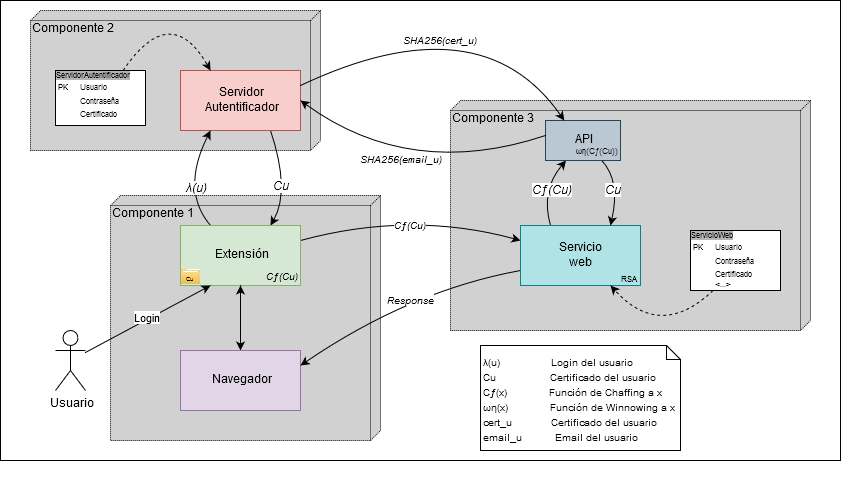
\includegraphics[width=15cm]{./imagenes/Analisis/ArquitecturaSistema.png}
        		\caption{Arquitectura General del Sistema}
	            \end{center}
	        \end{figure}    	
    	
    	%%%%%%%%%%%%%%%%%%%%%%%%%%%%%%%%%%%%%%%%%%%%%%%%%%%%%%%%%
		%                                                       %
		%                                                       %
		%                       DCU General                     %
		%                                                       %
		%                                                       %
		%%%%%%%%%%%%%%%%%%%%%%%%%%%%%%%%%%%%%%%%%%%%%%%%%%%%%%%%%
	    \section{Diagrama de casos de uso general.}
	         \begin{figure}[H]
        		\begin{center}
        		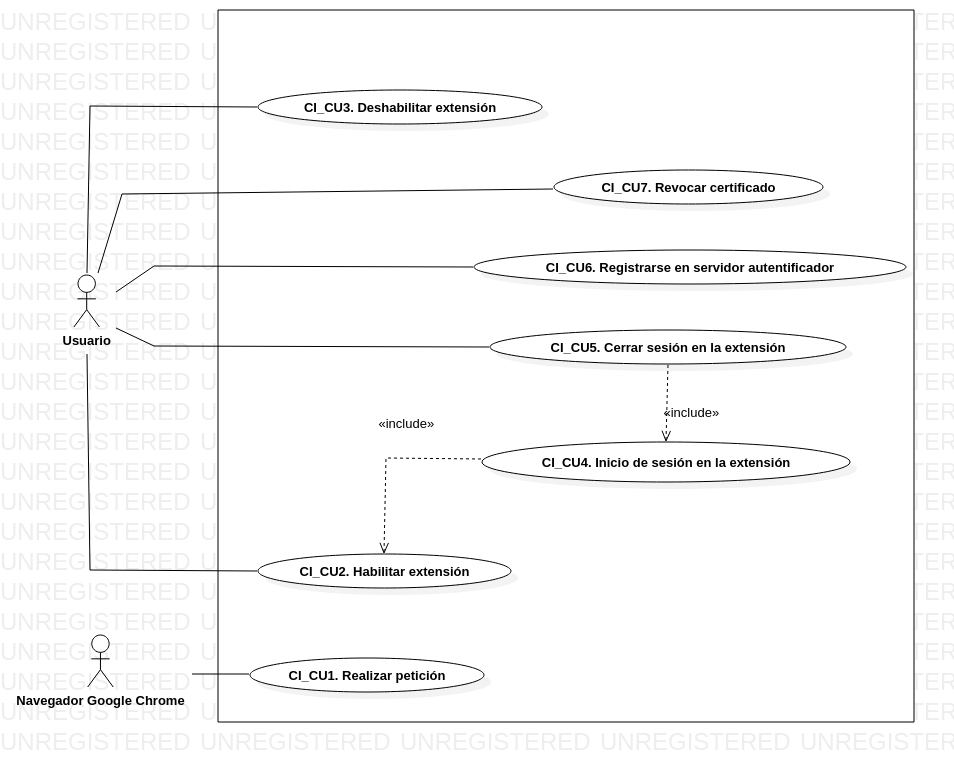
\includegraphics[width=13cm]{./imagenes/Analisis/UCD_General.png}
        		\caption{Diagrama de casos de uso general del sistema}
	            \end{center}
	        \end{figure}   
	        
	        NOTA: en la sección de desarrolla, cada prototipo describirá sus casos de uso correspondientes para su funcionamiento.
	        
	    %%%%%%%%%%%%%%%%%%%%%%%%%%%%%%%%%%%%%%%%%%%%%%%%%%%%%%%%%
		%                                                       %
		%                                                       %
		%                      Análisis PI                      %
		%                                                       %
		%                                                       %
		%%%%%%%%%%%%%%%%%%%%%%%%%%%%%%%%%%%%%%%%%%%%%%%%%%%%%%%%%
		\section{Prototipo I.}
			\subsection{Descripción.}
				En este prototipo se busca la creación de una extensión de Google Chrome que pueda interceptar una petición \acrshort{http} hecha por el mismo navegador mientras se encuentre habilitada, y así evitar que dicha petición sea mandada al servidor. Además, la extensión mostrará en otra pestaña del navegador información sobre la petición interceptada, con la finalidad de analizar los datos del encabezado HTTP. \\\\
				El propósito de realizar este prototipo es familiarizarse con el manejo de extensiones en el navegador Google Chrome; como es que podemos obtener la información que necesitamos para que posteriormente modifiquemos esta petición y la enviemos al servidor de prueba. 
			
			\subsection{Herramientas a usar.}
				\paragraph{Software. \\}
				Para el desarrollo de software de este prototipo, es necesario hacer mención de algunas de las siguientes herramientas, para tener una idea clara sobre qué herramientas estamos utilizando y porque es que las estamos utilizando:
				
				\paragraph{HTML5. \\}
				\acrlong{html} comenzó mucho tiempo atrás con una simple versión propuesta para crear la estructura básica de páginas web, organizar su contenido y compartir información, todo esto tenía la intención de comunicar información por medio de texto. El limitado objetivo de \acrshort{html} motivó a varias compañías a desarrollar nuevos lenguajes y programas para agregar características a la web nunca antes implementadas.   \\\\
				Dos de las opciones propuestas fueron Java y \Gls{Flash}; ambas fueron muy aceptadas y consideradas como el objetivo de la internet, sin embargo, con el crecimiento exponencial del internet, éste dejó de ser únicamente para los aficionados de los computadores y pasó a ser usado como un campo estratégico para los negocios y para la interacción social, ciertas limitaciones presentes en ambas tecnologías probaron ser una sentencia de muerte. Esta falta de integración resultó ser crítica y preparó el camino para la evaluación de un lenguaje del cual hablaremos un poco más a detalle después: JavaScript. Sin embargo, pese a su gran impacto, el mercado no terminó de adoptarlo plenamente y rápidamente su popularidad fue declinando, y el mercado terminó enfocando su atención a Flash. No fue hasta que los navegadores mejoraron su intérprete para JavaScript y la gente se empezaba a dar cuenta de las limitaciones que ofrecía Flash, que JavaScript fue implementado y comenzó a innovar la forma en la que se programaba la web. Al cabo de unos años, JavaScript, \acrshort{html} y \acrshort{css} eran considerados como la más perfecta combinación para evolucionar la Web. \\\\
				HTML5 es una mejora de esta combinación, lo que unió todos estos elementos. HTML5 propone estándares para cada aspecto de la Web y también un propósito claro para cada una de las tecnologías involucradas. A partir de esto, \acrshort{html} provee los elementos estructurales, CSS se concentra en como volver esta estructura utilizable y atractiva a la vista, y JavaScript tiene todo lo necesario para brindar dinamismo y construir aplicaciones web completamente funcionales. Cabe mencionar que HTML5 funciona diferente dependiendo del navegador y la versión en la que se esté trabajando, algunos soportan más carcterísticas o diferentes funcionalidades que otros.
				
				\paragraph{CSS3.\\}
				Ya se ha mencionado anteriormente como es que HTML5 fue evolucionando a un grado de combinación de estructura y diseño, sin embargo, la web demanda diseño y funcionalidad, no solamente organización estructural o definición de secciones, la función de CSS se concentra en volver la estructura de HTML utilizable y atractivo a la vista.\\
				
				Oficialmente CSS no tiene nada que ver con HTML4, no es parte de la especificación, es de hecho, un complemento desarrollado para superar las limitaciones y reducir la complejidad de HTML. Al principio, atributos dentro de las etiquetas HTML proveóan estilos esenciales para cada elemento, pero a medida que HTML evolucionó, la escritura de códigos se volvió más compleja y html por sí mismo no pudo satisfacer más las demandas de los diseñadores. En consecuencia a esta demanda, CSS fue adoptado como la forma de separar la estructura de la presentación, y ha ido creciendo y ganando importancia, pero siempre desarrollado en paralelo enfocado en las necesidades de los diseñadores y apartado de la estructura de HTML.\\
				
				La versión 3 de CSS sigue el mismo camino, pero esta vez con un mayor compromiso. La especificación de HTML5 fue desarrollada considerando CSS a cargo del diseño, Debido a esta consideración, la integración entre HTML y CSS es ahora vital para el desarrollo web y esta razón por la que cada vez que mencionamos HTML5 también estamos haciendo referencia a CSS3, aunque oficialmente se trate de dos tecnologías completamente separadas. Las nuevas características incorporadas en CSS3 están siendo implementadas e incluidas junto al resto de la especificación en navegadores compatibles con HTML5. 
				\cite{refElGranLibro}%Pag 19 pdf
				
				\paragraph {JavaScript. \\}
				JavaScript es considerado como el lenguaje de programación de \acrshort{html} y de la web. Es un lenguaje de programación fácil de usar y muy versátil para el ámbito de la comunicación en redes. Los programas, llamados "scripts", se ejecutan en el navegador (Mozilla, Google Chrome, Internet Explorer, etc.) normalmente consisten en unas funciones que son llamadas desde el propio \acrshort{html} cuando algún evento sucede.\\\\
				Su primera aproximación a un uso real, fue en mayor parte para "dar vida a una página web", como dar animaciones a un botón, interacciones en tiempo real, entre otras más. 
				JavaScript fue desarrollado por \Gls{NetScape}, a partir del lenguaje Java, que en ese momento tenía mucho auge y popularidad, y su principal diferencia es que JavaScript sólo "funciona" dentro de una página \acrshort{html}.\\
				JavaScript fue declarado como estándar del European Computer Manufacturers Association (ECMA) en 1997, y poco después, también fue estandarizado por ISO.\cite{refJavaScript} \\\\ 
				JavaScript es un lenguaje interpretado, usado mayormente como complemento de ciertos objetivos específicos, sin embargo, uno de las innovaciones que ayudó a JavaScript fue el desarrollo de nuevos motores de interpretación, creados para acelerar el procesamiento del código. La clave de los motores más exitosos fue transformar el código de Javascript en código máquina para obtener una velocidad de ejecución mejor que antes. Esto a la vez permitió superar viejas limitaciones de rendimiento y confirmar el lenguaje JavaScript como la mejor opción para la Web.\\\\
				
				Para aprovechar esta prometedora plataforma de trabajo ofrecida por los nuevos navegadores, JavaScript fue expandido en cuestión de portabilidad e integración, a la vez, interfaces de programación de aplicaciones (APIs) fueron incorporando por defecto con cada navegador para asistir a JavaScript en funciones elementales. El objetivo de esto, fue principalmente hacer disponible poderosas funciones a través de técnicas de programación sencillas y estándares, expandiendo el alcance del lenguaje y facilitando la creación de programas útiles para la Web.\cite{refElGranLibro}
				
				
				\paragraph{Hardware. \\}
				En el ámbito del hardware, utilizaremos los equipos de cómputo con los cuales contamos actualmente los integrantes de este equipo, los cuales se especificarán a continuación: 
				
				\begin{table}[H]
					\begin{tabular}{|p{3.5cm}||p{10cm}|}
						\rowcolor{guindapoli}
						\multicolumn{2}{|c|}{\textbf{\textcolor{white}{Equipo de hardware utilizado.}}}\\
						\hline
						\rowcolor{azulclaro}Marca & Asus\\
						\hline
						\rowcolor{white}Modelo & X550VC\\
						\hline
						\rowcolor{azulclaro}Procesador & Intel Core i5\\
						\hline
						\rowcolor{white}Tarjeta de video & NVidia GForce 720\\
						\hline
						\rowcolor{azulclaro}Memoria RAM & 12 GB\\
						\hline
						\rowcolor{white}Disco duro & 1TB\\
					\end{tabular}
				\end{table}
				
				\begin{table}[H]
					\begin{tabular}{|p{3.5cm}||p{10cm}|}
						\rowcolor{guindapoli}
						\multicolumn{2}{|c|}{\textbf{\textcolor{white}{Equipo de hardware utilizado.}}}\\
						\hline
						\rowcolor{azulclaro}Marca & HP\\
						\hline
						\rowcolor{white}Modelo & Pavilion g4\\
						\hline
						\rowcolor{azulclaro}Procesador & Intel Core i3\\
						\hline
						\rowcolor{white}Tarjeta de video & Intel Sandybridge Mobile\\
						\hline
						\rowcolor{azulclaro}Memoria RAM & 6 GB\\
						\hline
						\rowcolor{white}Disco duro & 500GB\\
					\end{tabular}
				\end{table}
			
			%%%%%%%%%%%%%%%%%%%%%%%%%%%%%%%%%%%%%%%%%%%%%%%%%%%%%%%%%
			%                                                       %
			%                                                       %
			%                REQUERIMIENTOS PI                     %
			%                                                       %
			%                                                       %
			%%%%%%%%%%%%%%%%%%%%%%%%%%%%%%%%%%%%%%%%%%%%%%%%%%%%%%%%%
            
			\subsection{Estudio de requerimientos.}
				\subsubsection{Requerimientos Funcionales.}
				{\setlength{\parindent}{12pt}
				\textbf{PI\_RF1. Interceptar petición \acrshort{http}.} La extensión deberá interceptar la petición \acrshort{http} del navegador, en cuanto el usuario realice alguna a través de éste.\\

				\textbf{PI\_RF2. Deshabilitar extensión.} El usuario podrá deshabilitar la extensión, para que ésta no vigile su actividad en el navegador.\\
				
				\textbf{PI\_RF3. Habilitar extensión.} El usuario podrá habilitar la extensión, para que ésta vigile las peticiones \acrshort{http}.\\
				
				\textbf{PI\_RF4. Validar petición.} La extensión deberá analizar la petición previamente recibida, y validar si ésta es HTTP(S) o no.\\
				
				\textbf{PI\_RF5. Mostrar petición.} La extensión deberá mostrar en otra pestaña del navegador, la información de la petición que se haya realizado.\\
				
				\textbf{PI\_RF6. Bloquear salida de petición.} La extensión deberá evitar que la petición salga a red, deteniendola cuando se le haya aplicado la función \textit{Chaffing} en el Prototipo II. 
		        }
				
				\subsubsection{Requerimientos no Funcionales.}
				{\setlength{\parindent}{12pt}
				
				\textbf{PI\_RNF1. Plataforma de implementación.} La extensión será implementada en el navegador Google Chrome Desktop.\\
				
				\textbf{PI\_RNF2. Versión del navegador} La extensión funcionará a partir de la versión 28.0.\\
				
				\textbf{PI\_RNF3. Tecnologías para la interfaz de usuario} Para el sistema se hará uso de \acrshort{html}5, JavaScript, \acrshort{css}3, JSON.\\
				
				\textbf{PI\_RNF4. Permitir ejecución de JavaScript en Google Chrome.} Para el correcto funcionamiento de la extensión, es necesario que se permita la ejecución de javascript en el navegador Google Chrome.\\
				
				\textbf{PI\_RNF5. Conexión a internet.} Para el funcionamiento de la extensión, no es necesario que se tenga conexión a internet.
				}
			
			\subsection{Reglas del negocio.}
				{\setlength{\parindent}{12pt}
			
				\textbf{PI\_RN1. Extensión habilitada.} En cuanto el usuario lo indique por medio de la \acrlong{iu}, la extensión deberá vigilar la actividad que éste realice en el navegador para interceptar una petición.\\
				\label{PI_RN1}
				
				\textbf{PI\_RN2. Extensión deshabilitada.} En cuanto el usuario lo indique por medio de la \acrlong{iu}, la extensión deberá dejar de vigilar la actividad que éste realice en el navegador.
				\label{PI_RN2}
				}
				
                \newpage
                
    	%%%%%%%%%%%%%%%%%%%%%%%%%%%%%%%%%%%%%%%%%%%%%%%%%%%%%%%%%
		%                                                       %
		%                                                       %
		%                      Análisis PII                     %
		%                                                       %
		%                                                       %
		%%%%%%%%%%%%%%%%%%%%%%%%%%%%%%%%%%%%%%%%%%%%%%%%%%%%%%%%%
		
		%%%%%%%%%%%%%%%%%%%%%%%%%%%%%%%%%%%%%%%%%%%%%%%%%%%%%%%%%
		%                                                       %
		%                                                       %
		%                      Análisis PII                     %
		%                                                       %
		%                                                       %
		%%%%%%%%%%%%%%%%%%%%%%%%%%%%%%%%%%%%%%%%%%%%%%%%%%%%%%%%%
		\section{Prototipo II.}
		    \subsection{Descripción.}
		    En este prototipo se busca que la extensión de Google Chrome pueda modificar la petición HTTP previamente interceptada. La modificación se hará sólo mientras la extensión esté habilitada, y tiene como objetivo inyectar el certificado autentificador en el encabezado del protocolo. Este certificado será simulado, sólo para este prototipo, por la misma extensión a partir de los datos del inicio de sesión, sin embargo, para los siguientes prototipos, se manejará una autoridad certificadora la cual recibirá los datos del inicio de sesión para que genere el certificado del usuario. Una vez que dicho certificado es inyectado, la extensión deberá liberar la petición para que salga a red.\\
		    
		    El propósito de este prototipo es utilizar la técnica de \textit{Chaffing and Winnowing} en este nuevo método de autentificación, para evitarle al usuario la tediosa tarea de ingresar sus credenciales cada vez que accede al servicio y brindarle la seguridad necesaria al iniciar de sesión.\\
		    
		    Para inyectar el certificado autentificador, es necesario crear un \textit{''patrón de chaffing''}, este patrón lo generaremos aleatoriamente para después mandarlo junto con la petición HTTP. Por el momento, dicho patrón no irá cifrado, ya que para esto es necesario la implementación del servidor del servicio web de prueba, para poder conocer su llave pública y cifrar el patrón. Sin embargo, en el prototipo III se implementará el servidor y con ello su cifrado asimétrico. El objetivo de mandar el patrón junto con el protocolo HTTP, es que el servidor pueda leer el patrón y realizar la etapa de \textit{winnowing}, para extraer el certificado.\\
            
            Los algoritmos necesarios para hacer el \textit{chaffing} son expuestos a continuación:\\
            
            \begin{algorithm}[H]
                \SetAlgoLined
                \KwData{requestHTTP, cert}
                \KwResult{patternChaffing}
                
                $lenHTTP \longleftarrow lenght(requestHTTP)$\;
                $lenCert \longleftarrow lenght(cert)$\;
                $lenPattern \longleftarrow lenHTTP + lenCert$\;
                $patternChaffing[lenPattern]$\;
                $count \longleftarrow 0$\;
                $y \longleftarrow lenHTTP \% 8$\;
                
                \While{$ count < lenCert$}{
                  $x \longleftarrow random \% lenPattern$\;
                  \If{$x <= 0 \quad \&\& \quad x < 8-y \quad \&\& \quad y \quad not \quad 0 $}{
                        $continue$\;
                   }
                   \If{$patternChaffing[x] == 0$}{
                        $patternChaffing[x] \longleftarrow 1$\;
                        $count \longleftarrow count + 1$\;
                   }
                 }
                $byteControl \longleftarrow 8-y$\;
                
                $putFirst(patternChaffing, byteControl)$\;
                \caption{Generación de patrón de chaffing}
            \end{algorithm}
            
            \newpage
            
            \begin{algorithm}[H]
                \SetAlgoLined
                \KwData{requestHTTP, cert, patternChaffing}
                \KwResult{protocolChaffed}
                
                $lenPattern \longleftarrow lenght(PatternChaffing)$\;
                $protocolChaffed[lenPattern]$
                $countHTTP \longleftarrow 0$\;
                $countCert \longleftarrow 0$\;
                
                $controlByte \longleftarrow getFirstByte(patternChaffing)$\;
                
                $entero \longleftarrow byteToInt(controlByte)$\;
                
                $countProtocolChaffed \longleftarrow entero$\;
                \While{$ countProtocolChaffed < lenPattern$}{
                  \eIf{$protocolChaffed[countProtocolChaffed] == 0$}{
                        $protocolChaffed[countProtocolChaffed] = cert[countCert]$\;
                        $countCert \longleftarrow countCert+1$\;
                   }{
                        $protocolChaffed[countProtocolChaffed] = requestHTTP[countHTTP]$\;
                        $countHTTP \longleftarrow countHTTP+1$\;
                   }
                   $countProtocolChaffed \longleftarrow countProtocolChaffed+1$\;
                }
                
                $randomShift \longleftarrow rdShift()$\;
                $binaryCicleRightShiftByByte(protocolChaffed, randomShift)$\;
                
                $putFirst(patternChaffing, randomShift)$\;
                
                \caption{Generación del chaffing}
            \end{algorithm}
		    
		   Primero vamos a analizar el algoritmo del \textit{patrón de chaffing} con un pequeño ejemplo (utilizaremos datos de variables más cortos); supongamos que nuestro certificado es el siguiente: 
		    \begin{center}
		        $C_k = MITZ057abZ251$
		    \end{center}
		    y utilizaremos el campo \textit{agent user} del header de la petición, lo cual tendrá lo siguiente:
		    \begin{center}
		        $P_{HTTP} = Mozilla5.5/Chrome8.1/Safari$
		    \end{center}
		    Entonces, nuestro patrón de chaffing terminará teniendo un tamaño de la longitud de los caracteres de nuestro certificado $+$ la longitud de los datos de la petición HTTP, que es nuestra variable \textit{lenPattern}, y en este caso será de una longitud de 41. A continuación vamos a utilizar un arreglo de banderas de ese tamaño que inicia con 0 todos sus valores, y que al final será nuestro patrón, (variable \textit{patternChaffing}). La idea es generar posiciones aleatorias dentro del rango del tamaño de \textit{lenPattern}, y poner un 1 en dicha posición si es que hay un 0, en caso que no se encuentre un 0 se repetirá el procedimiento obteniendo una posición aleatoria diferente, y esto se realizará el mismo número de veces del tamaño de nuestro certificado, para obtener un patrón de combinaciones entre los caracteres. Utilizaremos un contador para conseguir esto, aumentándolo cada vez que se obtenga un número aleatorio válido. En nuestro algoritmo, nuestra variable \textit{x} contiene la posición aleatoria donde se validará si en esa posición se puede poner un 1 o no.\\
		    
		    Existe un caso particular en el que la longitud de nuestro patrón será un múltiplo de 8\footnote{tamaño de bits en un byte}, en este caso puede crear un aleatorio dentro del rango de nuestro primer byte, para evitar esto pondremos una condición para que genere otro numero aleatorio'.  
		    
		    Al final necesitaremos un byte de control que le servirá al servidor saber a partir de donde empezará a realizar el \textit{winnowing}, esto se debe a que dependiendo del tamaño de la petición HTTP y su módulo 8 es donde empezará a checar los 0's y 1's; mandaremos este byte de control al principio de la petición con chaff.\\
		    %Agregar sobre la variable y Tenemos un caso en particular en el que puede ser posible que la longitud de la petición sea un múltiplo de 8, si esto sucede
		    
		    El segundo algoritmo realizará el chaff utilizando el patrón generado en el algoritmo anterior, obtendrá el byte de control y a partir de este, comenzará un contador para recorrer todos los bytes del patrón de chaffing, ademas contaremos con otros 2 contadores más: \textit{contCert} que irá recorriendo cada caracter de nuestro certificado, y \textit{countHTTP} que recorrerá los de la petición HTTP. Si la posición de éste contador se encuentra un 0, entonces quiere decir que debemos de agarrar el siguiente caracter de nuestro certificado, basándonos en nuestro contador, de la misma manera si se encuentra un 1, se agarrará el siguiente caracter de la petición, y estos se irán concatenando en una nueva cadena (\textit{protocolChaffed}). Al final, para incrementar la seguridad de nuestro \textit{chaff}, se realizará un corrimiento que se ve en la función de \text|it{binaryCicleRightShiftByByte}\footnote{Este corrimiento será cíclico y basado en el código ASCII, es decir, se escogerá el caracter de n bytes a su derecha módulo de 256.}.\\
		    
		    Por último se enviará al servidor el patrón de chaffing junto con el mismo chaff, así podrá saber como realizar el \textit{winowwing} para obtener los datos correspondientes del certificado.
		    
		    \subsection{Herramientas a usar.}
		        \paragraph{Software. \\}
				Para el desarrollo del software de este prototipo, utilizaremos las mismas tecnolog\'ias que en el prototipo anterior.
				
				\paragraph{CryptoJs. \\}
				CryptoJs es una colección estándar y segura de algoritmos criptográficos implementados para JavaScript usando las mejores practicas y patrones. Es rápida y tiene una interfaz consistente y simple. Cuenta con algoritmos tales como: Hasher Algorithms (SHA-1, SHA-2), Cipher Algorithms (DES, AES), Block Modes and Padding, por mencionar algunos. \cite{refCryptoJs} El objetivo de usar esta herramienta es usar los métodos ya implementados en \textit{CryptoJs} para la generación de código hash para una mejor y rápida ejecución del sistema.
				
				\paragraph{Wireshark. \\}
				Wireshark es una analizador de paquetes de red. Un analizador captura paquetes de red y muestra los datos del paquete con el mayor detalle posible. Ésta herramienta es software libre y es el mejor analizador de paquetes hoy en día. \cite{refWireshark} Utilizaremos Wireshark para analizar los paquetes que viajan a través de la red, en este caso la petición modificada la cual contiene el certificado y el patrón ocultados mediante el método \textit{Chaffing}.
				
				\begin{comment}
				\paragraph{API FileSystem \\}
				Consiste en una API muy útil para trabajar con archivos en el entorno de desarrollo de Google Chrome, soporta la entrada de archivos y directorios desde una computadora personal. La ventaja de esta API es que no es necesario acceder a todos los archivos del usuario, si no que se crea una especie de unidad virtual en donde se localizan los archivos que el usuario deseé utilizar, en este caso en la extensión. \cite{filesystemmozilla} 
				
				%\paragraph {hay que usar otra madre pero no se que alv. \\}
				\paragraph{OpenSSL}
				SSL (Secure Sockets Layer o capa de conexión segura) es un estándar de seguridad global que permite la transferencia de datos cifrados entre un navegador y un servidor web. Es utilizado por millones\cite{opensslmillones} de empresas e individuos en línea a fin de disminuir el riesgo de robo y manipulación de información confidencial (como números de tarjetas de crédito, nombres de usuario, contraseñas, correos electrónicos, etc.) por parte de hackers y ladrones de identidades. Básicamente, la capa SSL permite que dos partes tengan una "conversación" privada.
				Para establecer esta conexión segura, se instala en un servidor web un certificado SSL (también llamado "certificado digital") que cumple dos funciones: Autenticar la identidad del sitio web, garantizando a los visitantes que no están en un sitio falso y cifrar la información transmitida.
				Openssl es una api que proporciona un entorno adecuado para encriptar los datos enviados a otra computadora dentro de una red y a su vez desencriptarlos adecuadamente por el receptor, evitando así, el acceso a la información por intrusos con la utilización de sniffer.
				El conjunto de herramientas OpenSSL es una característica de FreeBSD que ofrece una capa cifrada de transporte sobre la capa normal de comunicación, permitiendo la combinación con muchas aplicaciones y servicios de red. 
                Uno de los usos más comunes de OpenSSL es ofrecer certificados para usar con aplicaciones de software. Estos certificados aseguran que las credenciales de la compañía o individuo son válidos y no son fraudulentos. Si el certificado en cuestión no ha sido verificado por uno de las diversas “autoridades certificadoras” o CA, suele generarse una advertencia al respecto. Una autoridad de certificados es una compañía, que firma certificados para validar credenciales de individuos o compañías. Este proceso tiene un costo asociado y no es un requisito imprescindible para usar certificados, aunque puede darle un poco de tranquilidad a los usuarios. \cite{openssl}
                %filesystemmozilla https://developer.mozilla.org/es/docs/Web/API/FileSystem
				% opensslmillones https://www.verisign.com/es_LA/website-presence/online/ssl-certificates/index.xhtml
				%openssl https://www.globalsign.com/es/centro-de-informacion-ssl/que-es-ssl/
				\end{comment}
				
				\paragraph{Hardware. \\}
				En el ámbito del hardware, utilizaremos los equipos de cómputo del prototipo anterior.
			
			
			%%%%%%%%%%%%%%%%%%%%%%%%%%%%%%%%%%%%%%%%%%%%%%%%%%%%%%%%%
			%                                                       %
			%                                                       %
			%                REQUERIMIENTOS PII                     %
			%                                                       %
			%                                                       %
			%%%%%%%%%%%%%%%%%%%%%%%%%%%%%%%%%%%%%%%%%%%%%%%%%%%%%%%%%
			
		    \subsection{Estudio de requerimientos.}
				\subsubsection{Requerimientos Funcionales.}
				{\setlength{\parindent}{12pt}
				
				\textbf{PII\_RF1. Inicio de sesi\'on en la extensi\'on.} La extensi\'on contar\'a con una interfaz para el ingreso de datos del usuario, donde ingresará un usuario y contraseña. \\   
                
                \textbf{PII\_RF2. Generación del certificado autentificador.} Para el prototipo 2 la generación del certificado autentificador se har\'a del lado del cliente, simulando la tarea de una entidad certificadora, permitiendo as\'i generar automáticamente esta llave la cual servir\'a para el proceso de \textit{chaffing} del mensaje en el protocolo HTTP. Dicho certificado se generará con base a los datos del PII\_RF1. Inicio de sesión.\\
                
                \textbf{PII\_RF3. Almacenamiento del certificado autentificador.} La extensi\'on deberá almacenar el certificado autentificador.\\
                
                \textbf{PII\_RF4. Generación de patrón de \textit{Chaffing}.} La extensión generará un patrón para poder implementar el método de \textit{Chaffing}. Este patrón será generado al azar, y es aquel que se usará para introducir el código autentificador en el protocolo HTTP.\\
                
				\textbf{PII\_RF5. Etapa de \textit{Chaffing}.} Por medio del m\'etodo \textit{Chaffing} se crearán paquetes para agregar al encabezado HTTP que se ha interceptado gracias al prototipo 1, utilizando el patrón de \textit{Chaffing} del requerimiento funcional PII\_RF4. Generación de patrón de \textit{Chaffing}\\
                    
                % \textbf{PII\_RF6. Cifrado del patrón de \textit{Chaffing}.} La extensión deberá cifrar el patrón generado para realizar la etapa de \textit{Chaffing}, y deberá colocarlo en el protocolo HTTP, para que el servidor lo pueda obtener, descifrar y así realizar la etapa de \textit{Winnowing}.\\
                    
                \textbf{PII\_RF6. Liberaci\'on de Petición.} Se liberar\'a el bloqueo a la petici\'on HTTP impuesto por el prototipo I una vez terminado el proceso de \textit{Chaffing}, para que la petici\'on pueda llegar al servidor modificado correspondiente.\\
                
                % \textbf{PII\_RF8. Recepción de la petición modificada en el servidor.} El servidor implementado deberá recibir la petición modificada por la extensión de Google Chrome.\\
                
                % \textbf{PII\_RF9. Impresión del servidor de la petición modificada.} El servidor deberá imprimir la petición recibida, previamente modificada por la extensión, para verificar los datos recibidos.\\
                
		        }
				
				\subsubsection{Requerimientos no Funcionales.}
				{\setlength{\parindent}{12pt}
				
				\textbf{PII\_RNF1. Tamaño del código autentificador.} El tamaño del archivo depende totalmente del tamaño de llave que se desea generar. Para este prototipo se hará uso de la función \textit{hash} tomando como argumentos el nombre de usuraio y contraseña del usuario que se desea generar el código de hash.\\
				
				\textbf{PII\_RNF2. Almacenado de archivo en la extensión.} Se necesita tener cargado el archivo en la API de Google Chrome, \textbf{Storage} para el correcto funcionamiento de la función \textit{Chaff} y así inyectarlo en la petición. \\
				
				\textbf{PII\_RNF3. Conexión a internet.} Para el funcionamiento de este prototipo, es necesario tener acceso a internet. \\
				
				}
		    
		    \subsection{Reglas del negocio.}
		    %Martin y Odell (1998) y Russel (1995) proponen que una regla de negocio es un restricción que opera sobre el sistema.
		        
            \textbf{PII\_RN1. Petición válida.} La extensión modificará la petición siempre y cuando se trate de una petición válida HTTP .\\
            \label{PII_RN1}
            
            \textbf{PII\_RN2. Extensión habilitada.} La modificación de la petición HTTP solo se podrá realizar mientras la extensión se encuentre habilitada.\\
            \label{PII_RN2}
            
            \textbf{PII\_RN3. Inicio de sesión de extensión por usuario.} Cada usuario que desee utilizar la extensión sólo deberá tener una cuenta con un usuario y una contraseña respectiva a este usuario. \\
            \label{PII_RN3}
            
            \textbf{PII\_RN4. Acceso a internet.} Se debe de contar con acceso a internet para que la extensión pueda enviar al servidor la petición modificada.\\
            \label{PII_RN4}
				
			\textbf{PII\_RN5. Longitud de código autentificador.} La longitud del código autentificador es de 32 caracteres, debido a que la función de MD5 es un algoritmo de codificación de 128 bits que genera un hash hexadecimal de 32 caracteres, independientemente de la longitud de la palabra de entrada (nombre de usuario y contraseña).\\
			\label{PII_RN5}
			
			\textbf{PII\_RN6. Longitud del campo de usuario.} La longitud del usuario no debe pasar de 20 caracteres, y mínimo será de 3 caracteres.\\
			\label{PII_RN6}
			
			\textbf{PII\_RN7. Longitud del campo contraseña.}
			La longitud de la contraseña no debe pasar de 16 caracteres, y mínimo sera de 8 caracteres.\\
			\label{PII_RN7}
			
			\textbf{PII\_RN8. Caracteres permitidos en campo usuario.} Los caracteres permitidos en el campo de usuario son unicamente símbolos alfanúmericos.\\
			\label{PII_RN8}
			
			\textbf{PII\_RN9. Caracteres permitidos en campo contraseña.} Los caracteres permitidos en el campo de contraseña son unicamente símbolos alfanúmericos.\\
			\label{PII_RN9}
			
			\textbf{PII\_RN10. Formato de contraseña.} La contraseña debe tener al menos un número y una letra mayúscula.\\
			\label{PII_RN10}
				
	    %   %   %   %   %   %   %   %   %   
		%		                        %
		%           DESARROLLO          %
		%                               %
	    %   %   %   %   %   %   %   %   %
	
	    %%%%%%%%%%%%%%%%%%%%%%%%%%%%%%%%%%%%%%%%%%%%%%%%%%%%%%%%%
		%                                                       %
		%                                                       %
		%                      Análisis PIII                    %
		%                                                       %
		%                                                       %
		%%%%%%%%%%%%%%%%%%%%%%%%%%%%%%%%%%%%%%%%%%%%%%%%%%%%%%%%%
	    \section{Prototipo III.}
	        \subsection{Descripción.}
	            Para este prototipo, vamos a implementar un servicio web de prueba para realizar la etapa de \textit{winnowing} a la petición HTTP que le llegue. Esto implica la modificación del servidor para que detecte este nuevo tipo de autentificación y la creación de un algoritmo que realice el \textit{winnowing} al protocolo. El servidor que usaremos será Apache.\\
	            Así mismo, el servicio web implementará un cifrado asimétrico (RSA), esto con la finalidad de que la extensión del prototipo anterior, pueda tomar la ''llave pública'' del servidor y cifrar el \textit{''patrón de chaffing''} que se mandará en la petición, para que sólo el servidor pueda descifrar este patrón con su ''llave privada''.
	            El propósito de este prototipo es poder obtener el certificado autentificador, para poder validarlo y dar acceso o no al usuario. Cabe mencionar que, la primera vez que el servidor reciba el certificado autentificador, pedirá que se ''inicie sesión'' con la finalidad de poder asociar el certificado a una cuenta; el inicio de sesión en el servicio web, sólo se hará una vez, ya que para las peticiones posteriores, el certificado ya tendrá una cuenta asociada a la cual dar acceso.
	            
	       % \subsection{Herramientas a usar.}
	        
	       % \subsection{Estudio de requerimientos.}
	        
	       % \subsection{Reglas del negocio.}
	    
	    %%%%%%%%%%%%%%%%%%%%%%%%%%%%%%%%%%%%%%%%%%%%%%%%%%%%%%%%%
		%                                                       %
		%                                                       %
		%                      Análisis PIV                     %
		%                                                       %
		%                                                       %
		%%%%%%%%%%%%%%%%%%%%%%%%%%%%%%%%%%%%%%%%%%%%%%%%%%%%%%%%%
	    \section{Prototipo IV.}
	        \subsection{Descripción.}
	            
	       % \subsection{Herramientas a usar.}
	        
	       % \subsection{Estudio de requerimientos.}
	        
	       % \subsection{Reglas del negocio.}
	        
	        
	%%%%%%%%%%%%%%%%%%%%%%%%%%%%%%%%%%%%%%%%%%%%%%%%%%%%%%%%%
	%                                                       %
	%                                                       %
	%                      Desarrollo                      %
	%                                                       %
	%                                                       %
	%%%%%%%%%%%%%%%%%%%%%%%%%%%%%%%%%%%%%%%%%%%%%%%%%%%%%%%%% 
	    
	\chapter{\textcolor{azulescom}{Desarrollo.}}
		\section{Prototipo I.}
			\subsection{Diagrama de casos de uso.}

				Diagrama de casos de uso general para el prototipo I.
				\begin{figure}[htb]
					\begin{center}
			    	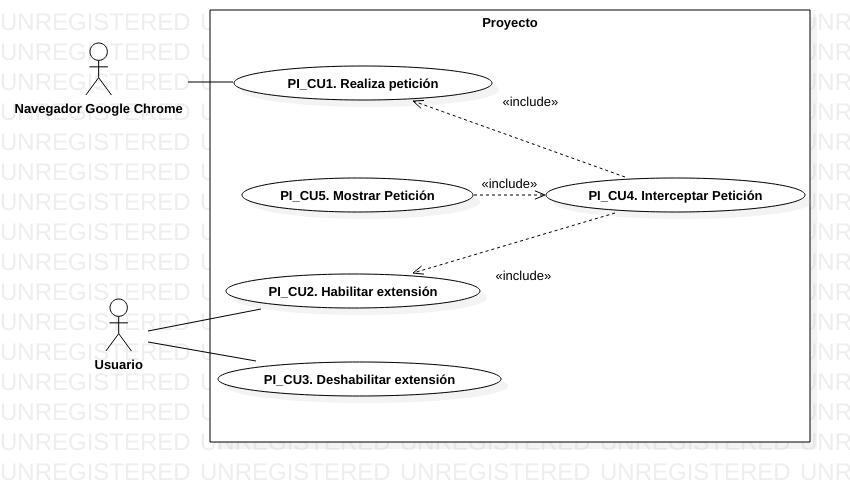
\includegraphics[width=15cm]{./imagenes/Desarrollo/Prototipo_1/UCD_P1.png}
						\caption{Diagrama de casos de uso del Prototipo I.}
					\end{center}
				\end{figure}\newpage	
					
			\subsection{Descripción de casos de uso.}
			
				%%%%%%%%%%%%%%%%
				        %%%%DESCRIPCIÓN PI_CU1
				%%%%%%%%%%%%%%%
				
				\begin{table}[H]
				\begin{tabular}{ |p{3.5cm}||p{9.5cm}|}
					\hline
					\rowcolor{guindapoli}
					\multicolumn{2}{|c|}{\textbf{\textcolor{white}{Caso de uso: PI\_CU1. Realizar petición.}}}\\
					\hline
					\rowcolor{azulfuerte}Concepto & Descripción\\
					\hline
					\cellcolor{azulclaro}Actor & 
					Navegador de Google Chrome.\\ 
					\hline
					\cellcolor{azulclaro}Propósito &
					Este caso de uso permite al navegador realizar una petición \acrshort{http}, ordenada por el usuario o un sistema externo.\\
					\hline
					\cellcolor{azulclaro}Entradas &
					URL del servicio web solicitado.\\
					\hline
					\cellcolor{azulclaro}Salidas &
					Petición \acrshort{http}.\\
					\hline
					\cellcolor{azulclaro}Pre-condiciones&
					Algún agente externo (Sistema o usuario) ha ordenado al navegador mandar una petición \acrshort{http}.\\
					\hline
					\cellcolor{azulclaro}Post-condiciones&
					Creación de la petición HTTP.\\
					\hline
					\cellcolor{azulclaro}Reglas del negocio&
					-\\
					\hline
					\cellcolor{azulclaro}Errores &
					La petición no se pudo realizar. \newline La petición no es tipo \acrshort{http}.\\					
					\hline
				\end{tabular}
				\caption[DCU: PI\_CU1]{Descripción CU: PI\_CU1}
				\end{table}
				
				\paragraph{... Trayectoria Principal ...}
				\begin{enumerate}
					\item \textbf{\textit{El Usuario}} o \textbf{\textit{El Sistema Externo}} realiza una petición \acrshort{http} en el navegador Google Chrome.\\
					\item \textbf{\textit{El navegador}} realiza la petición.\\
				\end{enumerate}
				\paragraph{... Fin de la Trayectoria Principal ...}
				
				\paragraph{... Trayectoria Alternativa 1 ...}
				\begin{enumerate}
					\item \textbf{\textit{El Usuario}} o \textbf{\textit{El Sistema Externo}} realiza una petición que no es \acrshort{http} en el navegador Google Chrome.\\
					\item \textbf{\textit{El navegador}} realiza la petición.					
				\end{enumerate}
				\paragraph{... Fin de la Trayectoria Alternativa 1 ...}
				
				\newpage
				%%%%%%%%%%%
				        %DESCRIPCIÓN PI_CU2
				%%%%%%%%%%
				
				\begin{table}[H]
				\begin{center}
				\begin{tabular}{ |p{3.5cm}||p{9.5cm}|}
					\hline
					\rowcolor{guindapoli}
					\multicolumn{2}{|c|}{\textbf{\textcolor{white}{Caso de uso: PI\_CU2. Habilitar extensión.}}}\\
					\hline
					\rowcolor{azulfuerte}Concepto & Descripción\\
					\hline
					\cellcolor{azulclaro}Actor & 
					Usuario.\\ 
					\hline
					\cellcolor{azulclaro}Propósito &
					Este caso de uso, permite al usuario habilitar la extensión, para que ésta sea capaz de ver todas las peticiones que realiza el navegador.\\
					\hline
					\cellcolor{azulclaro}Entradas &
					Indicación de habilitar extensión, mediante interfaz de usuario.\\
					\hline
					\cellcolor{azulclaro}Salidas &
					-\\
					\hline
					\cellcolor{azulclaro}Pre-condiciones&
					Estar en la \hyperref[UI_DESACTIVADO_4.8]{\textbf{UI servicio desactivado. Figura 4.8}}\\
					\hline
					\cellcolor{azulclaro}Post-condiciones&
					-\\
					\hline
					\cellcolor{azulclaro}Reglas del negocio&
					\hyperref[PI_RN1]{\textbf{PI\_RN1. Extensión habilitada.}}\\
					\hline
					\cellcolor{azulclaro}Errores &
					No se puede habiliar la extensión.\\
					\hline
				\end{tabular}
				\caption[DCU: PI\_CU2]{Descripción CU: PI\_CU2}
				\end{center}
				\end{table}
				
				\paragraph{... Trayectoria Principal ...}
				\begin{enumerate}
					\item \textbf{\textit{El usuario}} da click en el ícono de la extensión \img{imagenes/Desarrollo/Prototipo_1/escom.png}.
					\item \textbf{\textit{El usuario}} da click en el botón \img{imagenes/Desarrollo/Prototipo_1/boton_activar.png}.
					\item \textbf{\textit{La extensión}} empieza a vigilar las peticiones que se realicen a través del navegador.
				\end{enumerate}
				\paragraph{... Fin de la Trayectoria Principal ...}
				
				\paragraph{... Trayectoria Alternativa 1 ...}
				\begin{enumerate}
				    \item \textbf{\textit{La extensión}} no muestra el botón \img{imagenes/Desarrollo/Prototipo_1/boton_activar.png}, por ende el usuario no puede dar click.
				\end{enumerate}
				\paragraph{... Fin de la Trayectoria Alternativa 1 ...}
				
				\newpage
				%%%%%%%%%%%%%
				        %DESCRIPCIÓN PI_CU3
				%%%%%%%%%%%%
				
				\begin{table}[H]
				\begin{center}
				\begin{tabular}{ |p{3.5cm}||p{9.5cm}|}
					\hline
					\rowcolor{guindapoli}
					\multicolumn{2}{|c|}{\textbf{\textcolor{white}{Caso de uso: PI\_CU3. Deshabilitar extensión.}}}\\
					\hline
					\rowcolor{azulfuerte}Concepto & Descripción\\
					\hline
					\cellcolor{azulclaro}Actor & 
					Usuario.\\ 
					\hline
					\cellcolor{azulclaro}Propósito &
					Este caso de uso permite al usuario deshabilitar la extensión, para que ésta ignore todas las peticiones que se realicen por medio del navegador.\\
					\hline
					\cellcolor{azulclaro}Entradas &
					Indicación de deshabilitar extensión, mediante interfaz de usuario.\\
					\hline
					\cellcolor{azulclaro}Salidas &
					-\\
					\hline
					\cellcolor{azulclaro}Pre-condiciones&
				    Estar en la \hyperref[UI_ACTIVADO_4.7]{\textbf{UI servicio activado. Figura 4.7.}}\\
					\hline
					\cellcolor{azulclaro}Post-condiciones&	-\\
					\hline
					\cellcolor{azulclaro}Reglas del negocio&
					\hyperref[PI_RN2]{\textbf{PI\_RN2. Extensión deshabilitada}}\\
					\hline
					\cellcolor{azulclaro}Errores &
					No se puede deshabilitar la extensión.\\
					\hline
				\end{tabular}
				\caption[DCU: PI\_CU3]{Descripción CU: PI\_CU3}
				\end{center}
				\end{table}
			
				\paragraph{... Trayectoria Principal ...}
				\begin{enumerate}
					\item \textbf{\textit{El usuario}} da click en el ícono de la extensión \img{imagenes/Desarrollo/Prototipo_1/escom.png}.
					\item \textbf{\textit{El usuario}} da click en el botón \img{imagenes/Desarrollo/Prototipo_1/boton_desactivar.png}.
					\item \textbf{\textit{La extensión}} deja de vigilar las peticiones que se realicen a través del navegador.
				\end{enumerate}
				\paragraph{... Fin de la Trayectoria Principal ...}
				
		        \paragraph{... Trayectoria Alternativa 1 ...}
				\begin{enumerate}
				     \item \textbf{\textit{La extensión}} no muestra el botón \img{imagenes/Desarrollo/Prototipo_1/boton_desactivar.png}, por ende el usuario no puede dar click.
				\end{enumerate}
				\paragraph{... Fin de la Trayectoria Alternativa 1 ...}
				
				\newpage
				%%%%%%%%%%%%%%%%%%%%
				        %DESCRIPCIÓN PI_CU4
				        
				\begin{table}[H]
				\begin{center}
				\begin{tabular}{ |p{3.5cm}||p{9.5cm}|}
					\hline
					\rowcolor{guindapoli}
					\multicolumn{2}{|c|}{\textbf{\textcolor{white}{Caso de uso: PI\_CU4. Interceptar petición.}}}\\
					\hline
					\rowcolor{azulfuerte}Concepto & Descripción\\
					\hline
					\cellcolor{azulclaro}Actor & 
					 -.\\ 
					\hline
					\cellcolor{azulclaro}Propósito &
					Este caso de uso interceptará las peticiones HTTP que el navegador realice para su analisis.\\
					\hline
					\cellcolor{azulclaro}Entradas &
					Petición realizada por el navegador\\
					\hline
					\cellcolor{azulclaro}Salidas &
					-\\
					\hline
					\cellcolor{azulclaro}Pre-condiciones&
				    \textbf{PI\_CU1. Realizar petición} \newline \textbf{PI\_CU2. Habilitar extensión}\\
					\hline
					\cellcolor{azulclaro}Post-condiciones&
					\textbf{PI\_CU5. Mostrar Petición}\\
					\hline
					\cellcolor{azulclaro}Reglas del negocio&
					\hyperref[PI_RN2]{\textbf{PI\_RN1. Extensión habilitada}}\\
					\hline
					\cellcolor{azulclaro}Errores &
					La petición no se genera correctamente.\\
					\hline
				\end{tabular}
				\caption[DCU: PI\_CU4]{Descripción CU: PI\_CU4}
				\end{center}
				\end{table}
			
				\paragraph{... Trayectoria Principal ...}
				\begin{enumerate}
					\item \textbf{\textit{El usuario}} ingresa una URL en el navegador. 
					\item \textbf{\textit{El navegador}} genera una petición HTTP. 
					\item \textbf{\textit{La extensión}} Intercepta la petición realizada por el navegador para su análisis
				\end{enumerate}
				\paragraph{... Fin de la Trayectoria Principal ...}
				%%%%%%%%%%%%%%%%%%%
				
				\newpage
				%%%%%%%%%%%%%%%%%%%%
				        %DESCRIPCIÓN PI_CU5
				%%%%%%%%%%%%%%%%%%%
				
				\begin{table}[H]
				\begin{center}
				\begin{tabular}{ |p{3.5cm}||p{9.5cm}|}
					\hline
					\rowcolor{guindapoli}
					\multicolumn{2}{|c|}{\textbf{\textcolor{white}{Caso de uso: PI\_CU5. Mostrar Petición.}}}\\
					\hline
					\rowcolor{azulfuerte}Concepto & Descripción\\
					\hline
					\cellcolor{azulclaro}Actor & 
					-\\ 
					\hline
					\cellcolor{azulclaro}Propósito &
					Este caso de uso permite que la extensión cree una nueva pestaña para mostrar la petición interceptada.\\
					\hline
					\cellcolor{azulclaro}Entradas &
					Petición HTTP creada por el navegador.\\
					\hline
					\cellcolor{azulclaro}Salidas &
					Petición mostrada en una pestaña nueva.\\
					\hline
					\cellcolor{azulclaro}Pre-condiciones&
				    Caso de uso \textbf{PI\_CU4. Interceptar Petición}.\\
					\hline
					\cellcolor{azulclaro}Post-condiciones&	-\\
					\hline
					\cellcolor{azulclaro}Reglas del negocio&
					-\\
					\hline
					\cellcolor{azulclaro}Errores &
					No se puede crear una nueva pestaña.\newline
					No se puede recuperar la petición HTTP.\newline
					No se puede imprimir la petición en la nueva pestaña.\\
					\hline
				\end{tabular}
				\caption[DCU: PI\_CU5]{Descripción CU: PI\_CU5}
				\end{center}
				\end{table}
			
				\paragraph{... Trayectoria Principal ...}
				\begin{enumerate}
				    \item \textbf{\textit{La extensión}} recibe la petición HTTP a imprimir.
					\item \textbf{\textit{La extensión}} abre una nueva pestaña.
					\item \textbf{\textit{La extensión}} imprime la petición en \hyperref[UI_tabDatos_4.9]{\textbf{UI nueva pestaña con impresión del encabezado HTTP}}.
				\end{enumerate}
				\paragraph{... Fin de la Trayectoria Principal ...}

			%FIN DE LA DESCRIPCIÓN DE CASOS DE USO de PROTOTIPO 1
		
		    \subsection{Diagrama de flujo (DF).}
    			\begin{figure}[H]
    			    \begin{center} 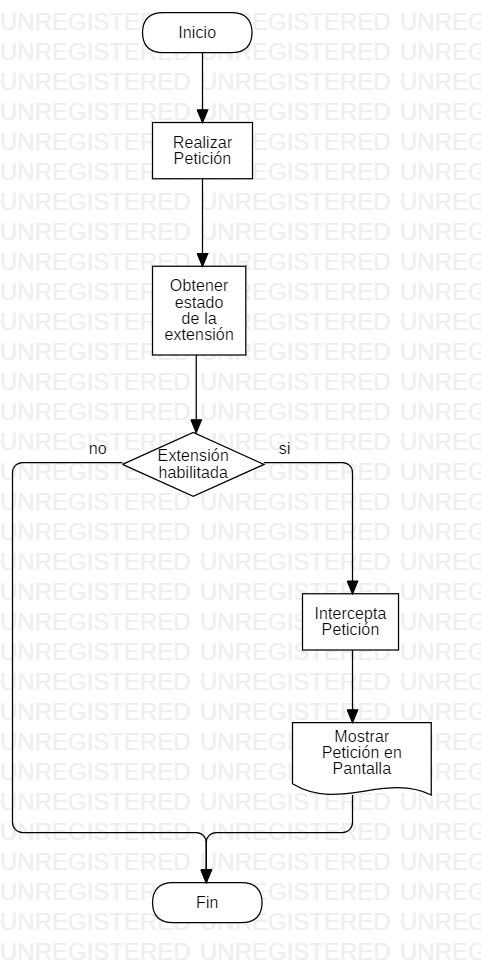
\includegraphics[width=0.8\textwidth]{imagenes/Desarrollo/Prototipo_1/DF_P1.png}
    			        \caption{Diagrama de flujo del Prototipo 1.}
    				\end{center}
    			\end{figure}
		        \subsubsection{Descripción diagrama de flujo.}
		        El primer paso del diagrama de flujo es esperar a que el usuario realice una petición web a algún servidor, luego obtener el estado actual de la extensión para saber si se encuentra habilitada o no, para luego realizar la comprobación correspondiente, es decir, "Extensión habilitada", en caso de que no se encuentre habilitada se acaba el flujo y ya no se realiza ninguna acción, en caso de que si se encuentre habilitada se intercepta la petici\'on HTTP y se evita que salga de la extensión, para este entonces se crea una nueva pestaña y se muestra toda la información de la petici\'on, hasta este paso damos por concluido el prototipo 1.
    			\subsection{Diagrama de flujo de datos (DFD).}
        			\begin{figure}[H]
        			    \begin{center}
    			        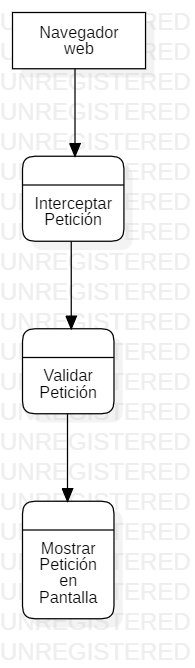
\includegraphics[width=0.5\textwidth]{imagenes/Desarrollo/Prototipo_1/DFD_P1.png}
    			        \caption{Diagrama de flujo de datos del Prototipo 1.}
    				\end{center}
    			\end{figure}
			    \subsubsection{Descripción diagrama de flujo de datos.}  
			    Para este diagrama solo nos limitamos a los datos que se utilizan en el prototipo uno los cuales son las peticiones tanto de salida como las de entrada, al inicio la extensión intercepta la petición, los cuales son datos que se validan para detectar cuales son HTTP y después de esto simplemente se muestran los datos en pantalla.
			    
			\subsection{Diagrama de clases.}
				\begin{figure}[H]
					\begin{center}	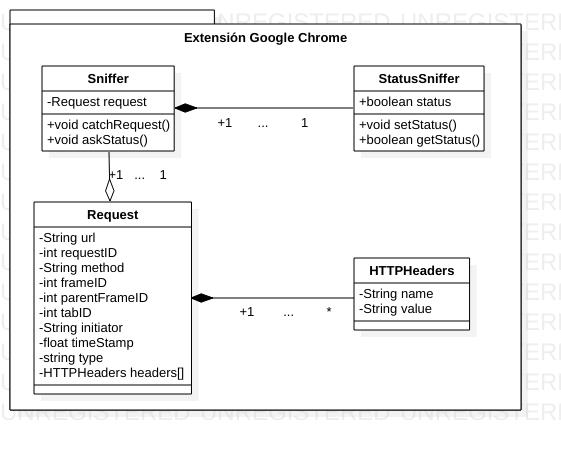
\includegraphics[width=13cm]{./imagenes/Desarrollo/Prototipo_1/DC_P1.png}
					\caption{Diagrama de clases del Prototipo I.}
					\end{center}
				\end{figure}
			
			\subsubsection{Descripción diagrama de clases.}
			    
			    \large StatusSniffer
			    \begin{enumerate}
    		        \item \textbf{status} : Variable que permite conocer y almacenar el status de la extensión (Habilitada/Deshabilitada).
    		        \begin{enumerate}
    		            \item Tipo de dato: \textbf{boolean}.
    		        \end{enumerate}
    		        Métodos
    		        \begin{enumerate}
    		            \item \textbf{setStatus()}: Se establece el valor del status, True (Está activada la extensión) o False (No está activa la extensión).
    		            \item \textbf{getStatus()}: Se obtiene el valor del status de la extensión, True o False.
    		        \end{enumerate}
			    \end{enumerate}
		        
	            \large Sniffer
			    \begin{enumerate}
    		        \item \textbf{request} : Variable que almacena los valores de la cabecera HTTP.
    		        \begin{enumerate}
    		            \item Tipo de dato: \textbf{Request}.
    		        \end{enumerate}
    		        Métodos
    		        \begin{enumerate}
    		            \item \textbf{catchRequest()}: Intercepta la petición para obtener los valores de la cabecera.
    		            \item \textbf{askStatus()}: Invoca al método \textit{getStatus()} de la clase StatusSniffer para conocer el status de la extensión.
    		        \end{enumerate}
			    \end{enumerate}
			    
			    \large Request
			    \begin{enumerate}
    		        \item \textbf{url} : Variable que almacena la URL requerida.
    		        \begin{enumerate}
    		            \item Tipo de dato: \textbf{String}.
    		        \end{enumerate}
    		        \item \textbf{requestID} : Variable que almacena el ID de la petición.
    		        \begin{enumerate}
    		            \item Tipo de dato: \textbf{int}.
    		        \end{enumerate}
    		        \item \textbf{method} : Variable que almacena el tipo de método de la petición, \textit{GET} o \textit{POST}.
    		        \begin{enumerate}
    		            \item Tipo de dato: \textbf{String}.
    		        \end{enumerate}
    		        \item \textbf{frameID} : Variable que almacena el tipo del frame.
    		        \begin{enumerate}
    		            \item Tipo de dato: \textbf{int}.
    		        \end{enumerate}
    		        \item \textbf{parentFrameID} : Variable que almacena el id del frame que envía la petición. 
    		        \begin{enumerate}
    		            \item Tipo de dato: \textbf{int}.
    		        \end{enumerate}
    		        \item \textbf{tabID} : Variable que almacena el ID del tab que toma lugar en la petición.
    		        \begin{enumerate}
    		            \item Tipo de dato: \textbf{int}.
    		        \end{enumerate}
    		        \item \textbf{initiator} : Variable que almacena el origen de la petición.
    		        \begin{enumerate}
    		            \item Tipo de dato: \textbf{String}.
    		        \end{enumerate}
    		        \item \textbf{timeStamp} : Variable que almacena la hora cuando se dispara la petición.
    		        \begin{enumerate}
    		            \item Tipo de dato: \textbf{float}.
    		        \end{enumerate}
    		        \item \textbf{type} : Variable que almacena el tipo de la petición.
    		        \begin{enumerate}
    		            \item Tipo de dato: \textbf{String}.
    		        \end{enumerate}
    		        \item \textbf{headers} : Variable de tipo Array que almacena los headers a ser enviados junto con la petición.
    		        \begin{enumerate}
    		            \item Tipo de dato: \textbf{HTTPHeaders}.
    		        \end{enumerate}
			    \end{enumerate}
			    
			    \large HTTPHeaders
			    \begin{enumerate}
    		        \item \textbf{name} : Variable que almacena el nombre del header a mandar junto con la petición.
    		        \begin{enumerate}
    		            \item Tipo de dato: \textbf{String}.
    		        \end{enumerate}
    		        \item \textbf{value} : Variable que almacena el contenido del header a enviar junto con la petición.
    		        \begin{enumerate}
    		            \item Tipo de dato: \textbf{String}.
    		        \end{enumerate}
			    \end{enumerate}
		    
		    
		    %%%%%%%%%%%%%%%%%%%%%%%%%%%%%
		    %%%%Diagrama de secuencia%%%%
		    %%%%%%%%%%%%%%%%%%%%%%%%%%%%%
			    
			\subsection{Diagrama de secuencia.}
		    	\begin{figure}[H]
				    \begin{center} 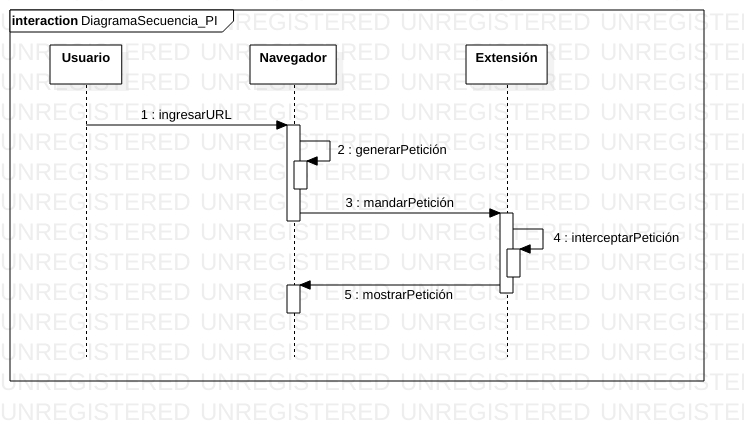
\includegraphics[width=15cm]{./imagenes/Desarrollo/Prototipo_1/SD_P1.png}
				    \caption{Diagrama de secuencia del Prototipo I.}
			        \end{center}
			    \end{figure}
			    
			    \subsubsection{Descripción del diagrama de secuencia.}
			    En este diagrama la secuencia de acciones que toman lugar para que la extensión pueda mostrar la petición interceptada. Dicha secuencia se explica en la siguiente lista.
			    \begin{enumerate}
			        \item Ingresar URL: este paso se refiere a cuando el usuario ingresa una URL. Dicha URL, por el momento, puede ser cualquiera ya que la extensión sólo la interceptará y modificará, sin embargo, para los siguientes prototipos sólo se utilizará la URL del servicio web de prueba que implementaremos.
			        \item Generar Petición: el navegador genera la petición HTTP que será mandada al servidor del servicio web. 
			        \item Mandar Petición: el navegador manda la petición al servidor del servicio web.
			        \item Interceptar Petición: La extensión interceptará la petición mandada por el navegador para que no salga a red.
			        \item Mostrar Petición: la extensión una vez habieando interceptado la petición, abrirá una nueva pestaña del navegador Google Chrome en donde mostrará la petición interceptada.
			    \end{enumerate}
            			        
			        
			        
			\subsection{Diagrama de actividades}
			    \begin{figure}[H]
				    \begin{center} 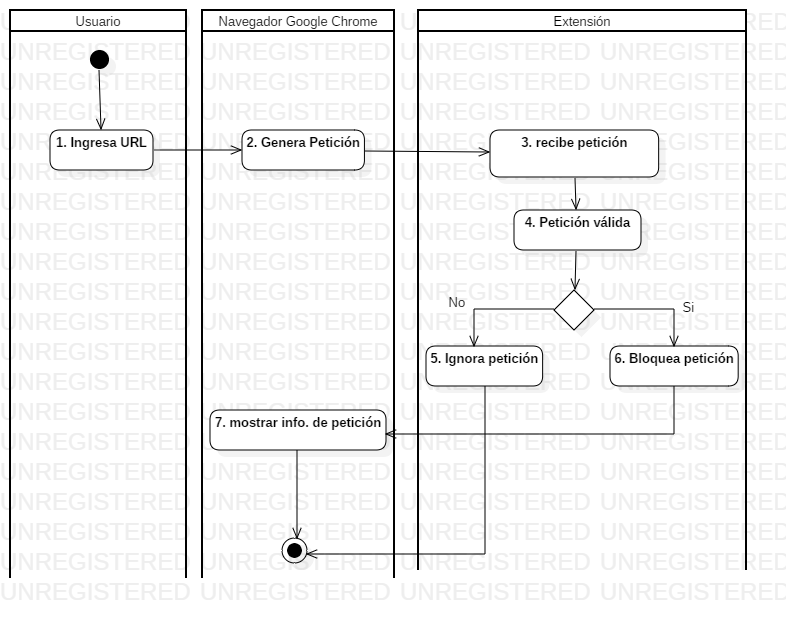
\includegraphics[width=11cm]{./imagenes/Desarrollo/Prototipo_1/DA_P1.png}
				        \caption{Diagrama de actividades Del Prototipo I.}
			        \end{center}
			    \end{figure}
			    
			\subsubsection{Descripción de diagrama de actividades.}
			Este diagrama muestra las actividades importantes que toman lugar en nuestro prototipo 1, enlistadas y explicadas como siguen: 
			
			\begin{enumerate}
			    \item \textbf{Usuario Ingresa URL:} El usuario ingresa en su navegador un URL el cual el desea ingresar.
			    \item \textbf{Navegador genera petición:} El navegador genera una petición con base al URL que el usuario ingreso previamente.
			    \item \textbf{Extensión recibe petición:}La extensión recibe la petición generada
			    \item \textbf{Extensión valida si la petición es HTTP:} La extensión valida el tipo de petición que recibe, si es de tipo HTTP o de algún otro.
			    \item \textbf{Extensión intercepta petición}: Si la petición es de tipo HTTP, entonces la extensión debe interceptar la petición, evitando que esta salga a red y al servidor.
			    \item \textbf{Mostrar la petición:} Una vez interceptada la petición, la extensión muestra información sobre esta en una nueva pestaña.
			    \item \textbf{Ignorar la petición:} Si la petición no es de tipo HTTP, entonces la extensión la ignora y no modifica o intercepta nada.
			\end{enumerate}
			
			    
			\subsection{Interfaz de usuario.}
			    
			    \begin{figure}[H]
					\begin{center}	
\includegraphics[width=9cm]{./imagenes/Desarrollo/Prototipo_1/escom.png}
						\caption{Logo de la extensión.}
					\end{center}
				\end{figure}
			  
			    \begin{figure}[H]
					\begin{center}	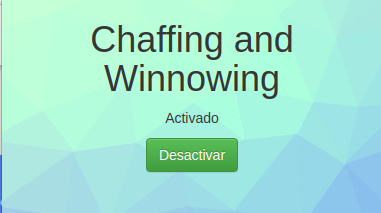
\includegraphics[width=13cm]{./imagenes/Desarrollo/Prototipo_1/UI_activado.png}
						\caption{Pantalla inicial. Servicio activado.}
					\end{center}
				\end{figure}
				\label{UI_ACTIVADO_4.7}
				
				\begin{figure}[H]
					\begin{center}	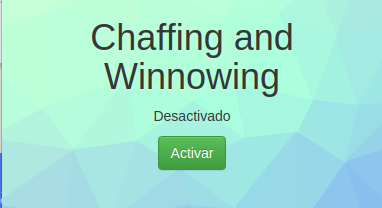
\includegraphics[width=13
					cm]{./imagenes/Desarrollo/Prototipo_1/UI_desactivado.png}
						\caption{Pantalla inicial. Servicio desactivado.}
					\end{center}
				\end{figure}
				\label{UI_DESACTIVADO_4.8}
				
				\begin{figure}[H]
					\begin{center}	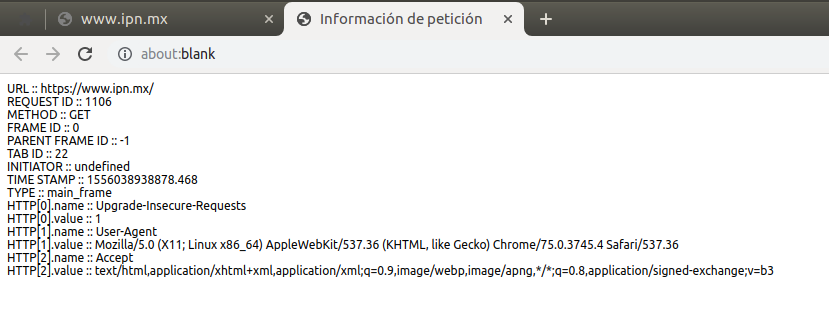
\includegraphics[width=13cm]{./imagenes/Desarrollo/Prototipo_1/UI_tabDatos.png}
						\caption{Nueva pestaña. Encabezado de petición.}
					\end{center}
				\end{figure}
				\label{UI_tabDatos_4.9}
			    
			\subsection{Requisitos de diseño.}
			   En este apartado, se especificarán las especificaciones de diseño para que el prototipo opere de forma correcta.
			   \subsubsection{Requisitos de ejecución sobre Google Chrome.}
			   Gracias a que Google Chrome es multiplataforma, esto es, funciona en varios sistemas operativos, el funcionamiento del Prototipo I depende exclusivamente de \textbf{tener instalado Google Chrome Stable o Google Chrome Developer} en la computadora local. Actualmente, este navegador para dispositivos móviles, no admite la instalación de extensiones, por lo que el funcionamiento depende también de tener una versión de \textbf{'Google Chrome Desktop'} instalada en la computadora. La extensión no podrá ejecutarse en Google Chrome para celulares o tabletas.\\
			   Sin embargo, para el Prototipo I utilizamos dos API's, llamadas \\ '\textit{chrome.webRequest}' y '\textit{chrome.storage}', las cuales están disponible sólo a partir de la\textbf{ versión 28}, por lo que, es necesario tener una versión igual o superior de este software.\\
			   Por otro lado, es \textbf{necesario que se permita que la extensión se ejecute sobre Google Chrome con ciertos permisos}, los cuales se exponen a continuación.
			   \begin{itemize}
			       \item Habilitar extensión: activado
			       \item Acceso al sitio web: en todos los sitios
			       \item Permitir acceso a URL de archivo: activado
			   \end{itemize}
			   
	    \newpage
			
		\section{Prototipo II.}
			%INICIO DE DESCRIPCION DE CASOS DE USO DE PROTOTIPO 2
			    \subsection{Diagrama de casos de uso}
			    
    			    \begin{figure}[H]
			            \begin{center}			                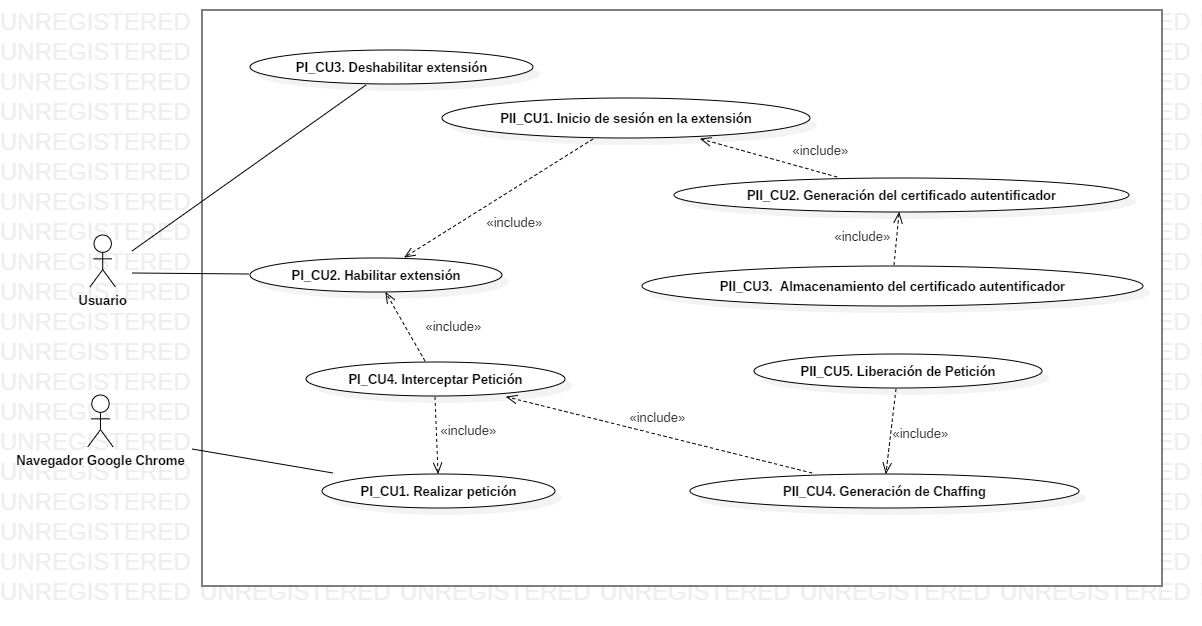
\includegraphics[width=16cm]{./imagenes/Desarrollo/Prototipo_2/UCD_P2.png}
    						\caption{Diagrama de casos de uso del Prototipo II.}
                        \end{center}    					
    				\end{figure}
			    
		        \subsection{Descripción de casos de uso.}
			    
				%%DESCRIPCIÓN PI_CU1
				\begin{table}[H]
    				\begin{tabular}{ |p{3.5cm}||p{9.5cm}|}
    					\hline
    					\rowcolor{guindapoli}
    					\multicolumn{2}{|c|}{\textbf{\textcolor{white}{Caso de uso: PII\_CU1. Inicio de sesión en la extensión}}}\\
    					\hline
    					\rowcolor{azulfuerte}Concepto & Descripción\\
    					\hline
    					\cellcolor{azulclaro}Actor & 
    					Usuario\\ 
    					\hline
    					\cellcolor{azulclaro}Propósito &
    					Este caso de uso permite al usuario poder iniciar sesión en la extensión para posteriormente obtener un código autentificador, basado en esos datos, al cual se le aplicará \textit{Chaffing}. \newline
    					Sólo se requerirá iniciar sesión una sola vez, ya que después, sólo es necesario subir el código generado para autentificarse en el servicio web.\\
    					\hline
    					\cellcolor{azulclaro}Entradas &
    					Usuario y Contraseña\\
    					\hline
    					\cellcolor{azulclaro}Salidas &
    					Código autentificador el cual hace referencia al usuario iniciado\\
    					\hline
    					\cellcolor{azulclaro}Pre-condiciones&
    					Haber instalado la extensión en el navegador Google Chrome y habiéndola habilitado.\\
    					\hline
    					\cellcolor{azulclaro}Post-condiciones&
    					Con los datos introducidos por el usuario, se obtendrá el código autentificador del mismo, para que lo guarde en su dispositivo y lo pueda subir después.\\
    					\hline
    					\cellcolor{azulclaro}Reglas del negocio&
    					\hyperref[PII_RN2]{PII\_RN2} \newline \hyperref[PII_RN3]{PII\_RN3} \newline
    					\hyperref[PII_RN6]{PII\_RN6} \newline
    					\hyperref[PII_RN7]{PII\_RN7} \newline
    					\hyperref[PII_RN8]{PII\_RN8} \newline
    					\hyperref[PII_RN9]{PII\_RN9} \newline
    					\hyperref[PII_RN10]{PII\_RN10} \\
    					\hline
    					\cellcolor{azulclaro}Errores &
    					No se encuentra usuario registrado \newline 
    					No se puede obtener el código autentificador\newline
    					No se pudo guardar el código autentificador\newline
    					Contraseña no válida\\					
    					\hline
    				\end{tabular}
				\caption[DCU: PII\_CU1]{Descripción CU: PII\_CU1}
				\end{table}
				
				\paragraph{... Trayectoria Principal ...}
				\begin{enumerate}
					\item \textbf{\textit{El Usuario}} realiza un inicio de sesión por primera vez en la extensión.
					\item \textbf{\textit{La extensión}} obtendrá los parametros de usuario y contraseña para generar un código autentificador único.
				\end{enumerate}
				\paragraph{... Fin de la Trayectoria Principal ...}
				
				\paragraph{... Trayectoria Alternativa 1 ...}
				\begin{enumerate}
					\item \textbf{\textit{El Usuario}} ingresa usuario y/o contraseña no validos.
					\item \textbf{\textit{La extensión}} no podrá obtener los datos del usuario.
				\end{enumerate}
				\paragraph{... Fin de la Trayectoria Alternativa 1 ...}
				
				\newpage
				
				%%DESCRIPCIÓN PI_CU2
				\begin{table}[H]
    				\begin{tabular}{ |p{3.5cm}||p{9.5cm}|}
    					\hline
    					\rowcolor{guindapoli}
    					\multicolumn{2}{|c|}{\textbf{\textcolor{white}{Caso de uso: PII\_CU2. Generación del certificado autentificador.}}}\\
    					\hline
    					\rowcolor{azulfuerte}Concepto & Descripción\\
    					\hline
    					\cellcolor{azulclaro}Actor & 
    					 -\\ 
    					\hline
    					\cellcolor{azulclaro}Propósito &
    					Este caso de uso generará un certificado para el usuario, basados en los datos que ingrese en la extensión (usuario y contraseña).\\
    					\hline
    					\cellcolor{azulclaro}Entradas &
    					Usuario y contraseña ingresados en la extensión.\\
    					\hline
    					\cellcolor{azulclaro}Salidas &
    					Certificado autentificador del usuario.\\
    					\hline
    					\cellcolor{azulclaro}Pre-condiciones&
    					Contar con la extensión habilitada. e ingresar un usuario y contraseña\\
    					\hline
    					\cellcolor{azulclaro}Post-condiciones&
    					 -\\
    					\hline
    					\cellcolor{azulclaro}Reglas del negocio&
    				    \hyperref[PII_RN6]{PII\_RN6.} \newline
    				    \hyperref[PII_RN7]{PII\_RN7.} \newline
    				    \hyperref[PII_RN8]{PII\_RN8.} \newline
    				    \hyperref[PII_RN9]{PII\_RN9.} \newline
    				    \hyperref[PII_RN10]{PII\_RN10.} \\
    					\hline
    					\cellcolor{azulclaro}Errores &
    					Error al generar el certificado.\\
    					\hline
    				\end{tabular}
				\caption[DCU: PII\_CU2]{Descripción CU: PII\_CU2}
				\end{table}
				\label{PII_CU2}
				
				\paragraph{... Trayectoria Principal ...}
				\begin{enumerate}
					\item \textbf{\textit{La extensión}} generará un código autentificador basado en los datos ingresados por el usuario.
				\end{enumerate}
				\paragraph{... Fin de la Trayectoria Principal ...}
				
				\paragraph{... Trayectoria Alternativa 1 ...}
				\begin{enumerate}
				    \item \textbf{\textit{La extensión}} no puede generar el código autentificador.
					\item \textbf{\textit{La extensión}} mostrará al usuario un mensaje de dicho error.
				\end{enumerate}
				\paragraph{... Fin de la Trayectoria Alternativa 1 ...}
				
				\newpage

				%
				%
				%       DESCRIPCIÓN PII_CU3
			    %
                %
                
				\begin{table}[H]
    				\begin{tabular}{ |p{3.5cm}||p{9.5cm}|}
    					\hline
    					\rowcolor{guindapoli}  					\multicolumn{2}{|c|}{\textbf{\textcolor{white}{Caso de uso: PII\_CU3. Almacenamiento del certificado autentificador.}}}\\
    					\hline
    					\rowcolor{azulfuerte}Concepto & Descripción\\
    					\hline
    					\cellcolor{azulclaro}Actor & 
    					-\\ 
    					\hline
    					\cellcolor{azulclaro}Propósito &
    					Este caso de uso permite que la extensión guarde el certificado autentificador, para que el usuario no tenga que hacerlo por el mismo. De esta manera, la extensión tendrá acceso al certificado cada que éste sea requerido.\newline El lugar donde se guarda dicho certificado es en ''Google Chrome Storage'', una zona de memoria que Google Chrome nos brinda al desarrollar una extensión para el navegador.\\
    					\hline
    					\cellcolor{azulclaro}Entradas &
    					Certificado autentificador.\\
    					\hline
    					\cellcolor{azulclaro}Salidas &
    					-\\
    					\hline
    					\cellcolor{azulclaro}Pre-condiciones&
    					Haber terminado el caso de uso \textbf{\hyperref[PII_CU2]{PII\_CU2. Generación del certificado autentificador}}. \\
    					\hline
    					\cellcolor{azulclaro}Post-condiciones&
    					-\\
    					\hline
    					\cellcolor{azulclaro}Reglas del negocio&
    					\hyperref[PII_RN5]{PII\_RN5. Longitud del certificado autentificador.}\\
    					\hline
    					\cellcolor{azulclaro}Errores &
    				    No se puede almacenar el certificado autentificador.\\
    					\hline
    				\end{tabular}
				\caption[DCU: PII\_CU3]{Descripción CU: PII\_CU3}
				\end{table}
				
				\paragraph{... Trayectoria Principal ...}
				\begin{enumerate}
				    \item \textbf{\textit{La extensión}} ha creado el certificado autentificador.
				    \item \textbf{\textit{La extensión}} guarda el certificado en storage.
				    \item \textbf{\textit{La extensión}} muestra al usuario el siguiente mensaje ''El certificado fue guardado con éxito'' en la pantalla \textbf{INSERT UI AVISO DE GUARDADO EXITOSO}
				\end{enumerate}
				\paragraph{... Fin de la Trayectoria Principal ...}
				
				\paragraph{... Trayectoria Alternativa 1 ...}
				\begin{enumerate}
				    \item \textbf{\textit{La extensión}} no ha creado el certificado autentificador.
					\item \textbf{\textit{La extensión}} no guarda el certificado autentificador en storage. 
					\item \textbf{\textit{La extensión}} muestra al usuario el siguiente mensaje ''No se encuentra certificado'' en la pantalla \textbf{INSERT UI AVISO DE CERTIFICADO NO ENCONTRADO}
				\end{enumerate}
				\paragraph{... Fin de la Trayectoria Alternativa 1 ...}
				
					\paragraph{... Trayectoria Alternativa 2 ...}
				\begin{enumerate}
				    \item \textbf{\textit{La extensión}} ha creado  el certificado autentificador.
					\item \textbf{\textit{La extensión}} no puede guardar el certificado autentificador en storage. 
					\item \textbf{\textit{La extensión}} muestra al usuario el siguiente mensaje ''No se pudo guardar el certificado'' en la pantalla \textbf{INSERT UI AVISO DE GUARDADO FALLIDO}
				\end{enumerate}
				\paragraph{... Fin de la Trayectoria Alternativa 2 ...}
				
				\newpage
			
			%
			%   DESCRIPCIÓN PI_CU5
			%
				\begin{table}[H]
    				\begin{tabular}{ |p{3.5cm}||p{9.5cm}|}
    					\hline
    					\rowcolor{guindapoli}
    					\multicolumn{2}{|c|}{\textbf{\textcolor{white}{Caso de uso: PII\_CU5. Liberación de Petición.}}}\\
    					\hline
    					\rowcolor{azulfuerte}Concepto & Descripción\\
    					\hline
    					\cellcolor{azulclaro}Actor & 
    					Navegador de Google Chrome\\ 
    					\hline
    					\cellcolor{azulclaro}Propósito &
    					Este caso de uso permite al Navegador de Google Chrome liberar la petición una vez que haya sido modificada por la extensión. Dentro de la petición se incluye el codigo autentificador junto con el patrón a utilizar en el proceso de \textit{Winnowing} una vez que sea recibido por el servidor.\\
    					\hline
    					\cellcolor{azulclaro}Entradas &
    					Petición\\
    					\hline
    					\cellcolor{azulclaro}Salidas &
    					Petición modificada enviada en red al servidor.\\
    					\hline
    					\cellcolor{azulclaro}Pre-condiciones&
    					Haber completado exitosamente el proceso de \textit{Chaffing} al igual que la creación del patrón, e inyectarlo en la petición.\\
    					\hline
    					\cellcolor{azulclaro}Post-condiciones&
    					Con los datos generados (Código Chaffing y patrón) generados por la extensión, se deben de inyectar en la petición para poder ser enviada al servidor a traves de la red.\\
    					\hline
    					\cellcolor{azulclaro}Reglas del negocio&
    					\hyperref[PII_RN1]{PII\_RN1} \newline \hyperref[PII_RN2]{PII\_RN2} \newline
    					\hyperref[PII_RN3]{PII\_RN3} \newline
    					\hyperref[PII_RN4]{PII\_RN4} \\
    					\hline
    					\cellcolor{azulclaro}Errores &
    					No se cuenta con acceso a internet \newline
    					Hay un error de estructura en la petición \\		
    					\hline
    				\end{tabular}
				\caption[DCU: PII\_CU5]{Descripción CU: PII\_CU5}
				\end{table}
				
				\paragraph{... Trayectoria Principal ...}
				\begin{enumerate}
					\item \textbf{\textit{El Navegador Google Chrome}} realiza una petición con el encabezado HTTP modificado, el cual contiene dentro del apartado \textit{headers} del encabezado HTTP el certificado modificado con el proceso de \textit{Chaffing} y el patrón que ayudará al servidor al momento de hacer el proceso de \textit{Winnowing}.
					\item \textbf{\textit{El analizador Wireshark}} captura la petición generada y muestra el encabezado modificado. Esto con el fin de mostrar que se ha generado el certificado y se ha modificado exitosamente con el proceso \textit{Chaffing}.				
					\end{enumerate}
				\paragraph{... Fin de la Trayectoria Principal ...}
				
				\paragraph{... Trayectoria Alternativa 1 ...}
				\begin{enumerate}
					\item \textbf{\textit{El Navegador de Google Chrome}} no puede establecer una conexión con el servidor debido a que no se cuenta con acceso a internet.
					\item \textbf{\textit{El analizador Wireshark}} no podrá obtener los datos del encabezado, ya que no capturará la petición.
				\end{enumerate}
				\paragraph{... Fin de la Trayectoria Alternativa 1 ...}
			
			\newpage
				
			\subsection{Diagrama de flujo de datos (DFD).}
			    \begin{figure}[htb]
					\begin{center}
			    	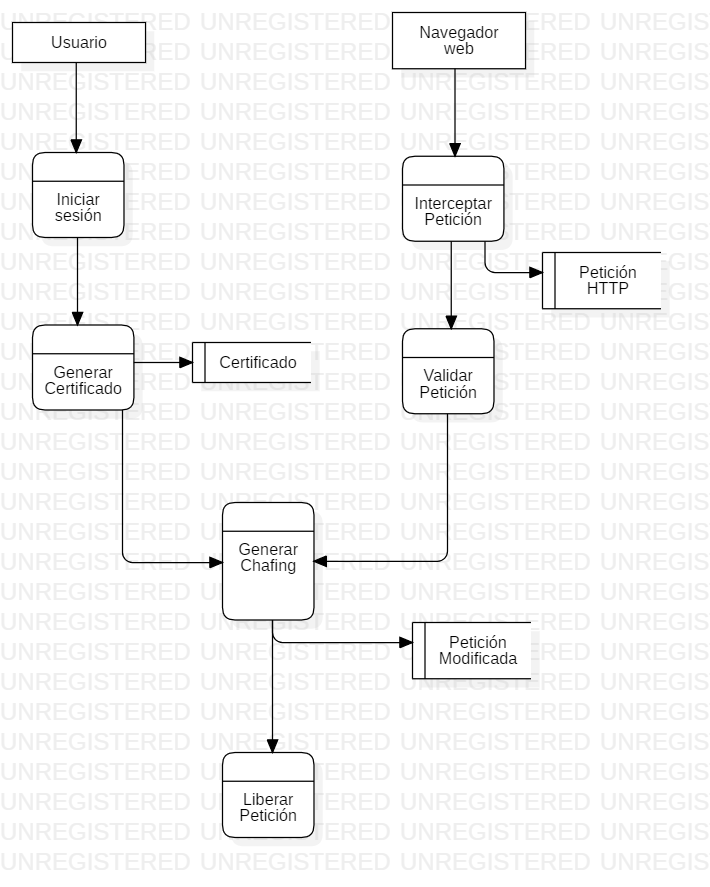
\includegraphics[width=10cm]{./imagenes/Desarrollo/Prototipo_2/DFD_P2.png}
						\caption{Diagrama de flujo de datos de Prototipo 2.}
					\end{center}
				\end{figure}
			    \newpage
			    
			    \subsubsection{Descripción diagrama de flujo de datos.}
			    Para este prototipo, el usuario podrá pedirle a la extensión que le genere un código autentificador (en este prototipo este código se obtendrá simulando el uso de una autoridad certificadora para obtenerlo) una vez que pueda obtenerlo, podrá guardar y escoger el código autentificador que vaya a utilizar la extensión (el previamente obtenido). El propósito general de este prototipo es que una vez que se tiene este código autentificador (certificado), se inyecte cifrado en la petición y se mande al servidor, donde este lo utilizará en los siguientes prototipos. 
			    
			    La información que queremos que viaje desde la extensión hasta el servidor es la petición modificada que tendrá todos los datos necesarios para que pueda descifrarlo correctamente, para que posteriormente el servidor pueda descifrarlo. Alamcenaremos el código autentificador para que el usuario tenga la confianza de poder cambiarlo cuando el gusté si siente que puede ser vulnerable, o cuando el certificado expire y sea necesario renovarlo. Cuando la extensión detecte que el usuario quiera ingresar a una página que requiera de un login, este empezará todo el proceso de \textit{chaff}, que es donde genera el patrón para introducir los datos de cierta manera y orden de modo que no pueda ser entendible para cualquiera que llegue a interceptar esta petición, poner ese chaff junto con el certificado cifrado en la petición y mandarlo al servidor, de esta forma la información viajara segura. 
			    
			    Para asegurarnos de que la petición se pudo generar bien, y de que llegará al servidor sin ningún problema, vamos a modificar el código fuente del servidor Apache para que muestre la información de la petición que recibe, esto es para fines únicamente de pruebas del desarrollo de este prototipo.
			
			\subsection{Diagrama de clases.}
			
    			\begin{figure}[H]
    				\begin{center}	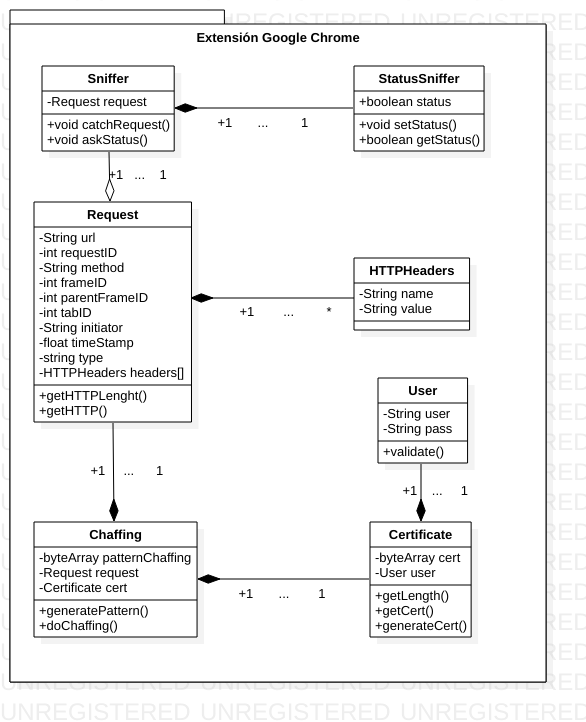
\includegraphics[width=13cm]{./imagenes/Desarrollo/Prototipo_2/DC_P2.png}
    				\caption{Diagrama de clases de Prototipo 2.}
    				\end{center}
    			\end{figure}
			    
			    \newpage
			    \subsubsection{Descripción de diagrama de clases}
			    \large User
			    \begin{enumerate}
    		        \item \textbf{user} : Variable que permite almacenar el valor del campo nombre de usuario.
    		        \begin{enumerate}
    		            \item Tipo de dato: \textbf{String}. \item Longitud de caracteres: \textbf{20 caracteres}.
    		            \item Restricciones: La cadena sólo puede tener símbolos alfanuméricos 
    		        \end{enumerate}
    		        \item \textbf{pass} : Variable que permite almacenar el valor del campo contraseña.
    		        \begin{enumerate}
    		            \item Tipo de dato: \textbf{String}. \item Longitud de caracteres: \textbf{16 caracteres}.
    		            \item Restricciones: Al menos un \textbf{número} y \textbf{una letra mayúscula}. La cadena sólo puede tener símbolos alfanuméricos.
    		        \end{enumerate}
    		        
    		        Métodos
    		        
    		        \begin{enumerate}
    		            \item validate() : Método que valida que los valores de las variables sean válidos.
    		        \end{enumerate}
			    \end{enumerate}
			        
		        \paragraph{}
	            \large Certificate
			    \begin{enumerate}
    		        \item \textbf{cert} : Variable que permite almacenar el valor del certificado autentificador.
    		        \begin{enumerate}
    		            \item Tipo de dato: \textbf{byte []}.
    		            \item Longitud: \textbf{32 bytes}.
    		        \end{enumerate}
    		        \item \textbf{user} : Variable que permite almacenar el usuario actual que se está utilizando.
    		        \begin{enumerate}
    		            \item Tipo de dato: \textbf{User}.
    		        \end{enumerate}
    		        
    		        Métodos:
    		        \begin{enumerate}
    		            \item getLenght() : método que devuelve la longitud del certificado.
    		            \item getCert() : método que devuelve el certificado.
    		            \item generateCert() : método que genera el certificado con base a los datos del usuario.
    		        \end{enumerate}
			    \end{enumerate}
			    
			    \paragraph{}
	            \large Chaffing
			    \begin{enumerate}
    		        \item \textbf{patternChaffing} : Variable que permite almacenar el patrón de \textit{chaffing}.
    		        \begin{enumerate}
    		            \item Tipo de dato: \textbf{byte []}.
    		            \item Longitud: \textbf{HTTP.Lenght() + cert.Lenght()}.
    		        \end{enumerate}
    		        \item \textbf{request} : Variable que permite almacenar la petición HTTP.
    		        \begin{enumerate}
    		            \item Tipo de dato: \textbf{Request}.
    		        \end{enumerate}
    		        \item \textbf{cert} : Variable que permite almacenar el certificado del usuario.
    		        \begin{enumerate}
    		            \item Tipo de dato: \textbf{Certificate}.
    		        \end{enumerate}
    		        
    		        Métodos:
    		        \begin{enumerate}
    		            \item generatePattern() : método que genera el patrón de \textit{chaffing}.
    		            \item doChaffing() : método que realiza el chaffing en la petición HTTP.
    		        \end{enumerate}
			    \end{enumerate}

        \subsection{Diagrama de secuencia.}       
           \begin{figure}[H]
				\begin{center}
		    	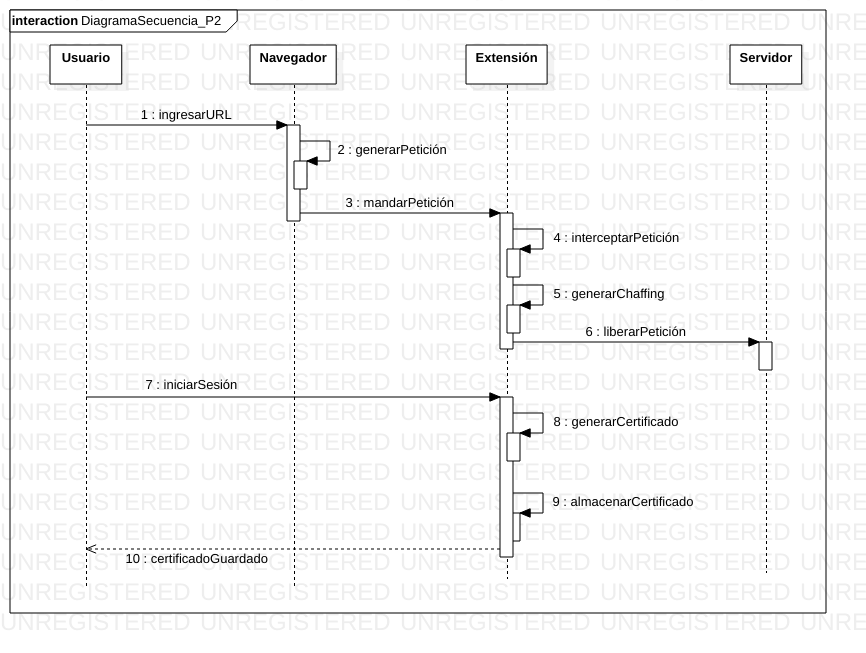
\includegraphics[width=15cm]{./imagenes/Desarrollo/Prototipo_2/SD_P2.png}
				\caption{Diagrama de secuencia del Prototipo 2.}
				\end{center}
			\end{figure}
			
			\subsubsection{Descripción del diagrama de secuencia.}
			
			Para este prototipo hemos agregado pasos al diagrama de secuencia, los cuales se describen a continuación.\\
			El primer paso es \textit{\textbf{iniciar sesión}}, para que la extensión obtenga los datos del usuario y pueda \textit{\textbf{generar el certificado}}, el cual es el segundo paso. Después, es necesario \textit{\textbf{almacenar el certificado}} para que la extensión tenga acceso a éste cuando lo requiera. Esta secuencia termina cuando la extensión le notifica al usuario el estatus del \textit{\textbf{certificado guardado}}.
			
			En la segunda secuencia para el funcionamiento de este prototipo, modificamos el anterior diagrama para cumplir con los requerimientos de éste. Ahora, después de \textit{\textbf{interceptar la petición}}, la extensión hará el paso de \textit{\textbf{generar chaffing}}, para poder inyectar el certificado autentificador en el protocolo HTTP. Finalmente, la extensión \textit{\textbf{liberará la petición}} para que salga a red y pueda llegar al servidor.
			
		
		
		\subsection{Diagrama de actividades}
		    \begin{figure}[H]
				\begin{center}	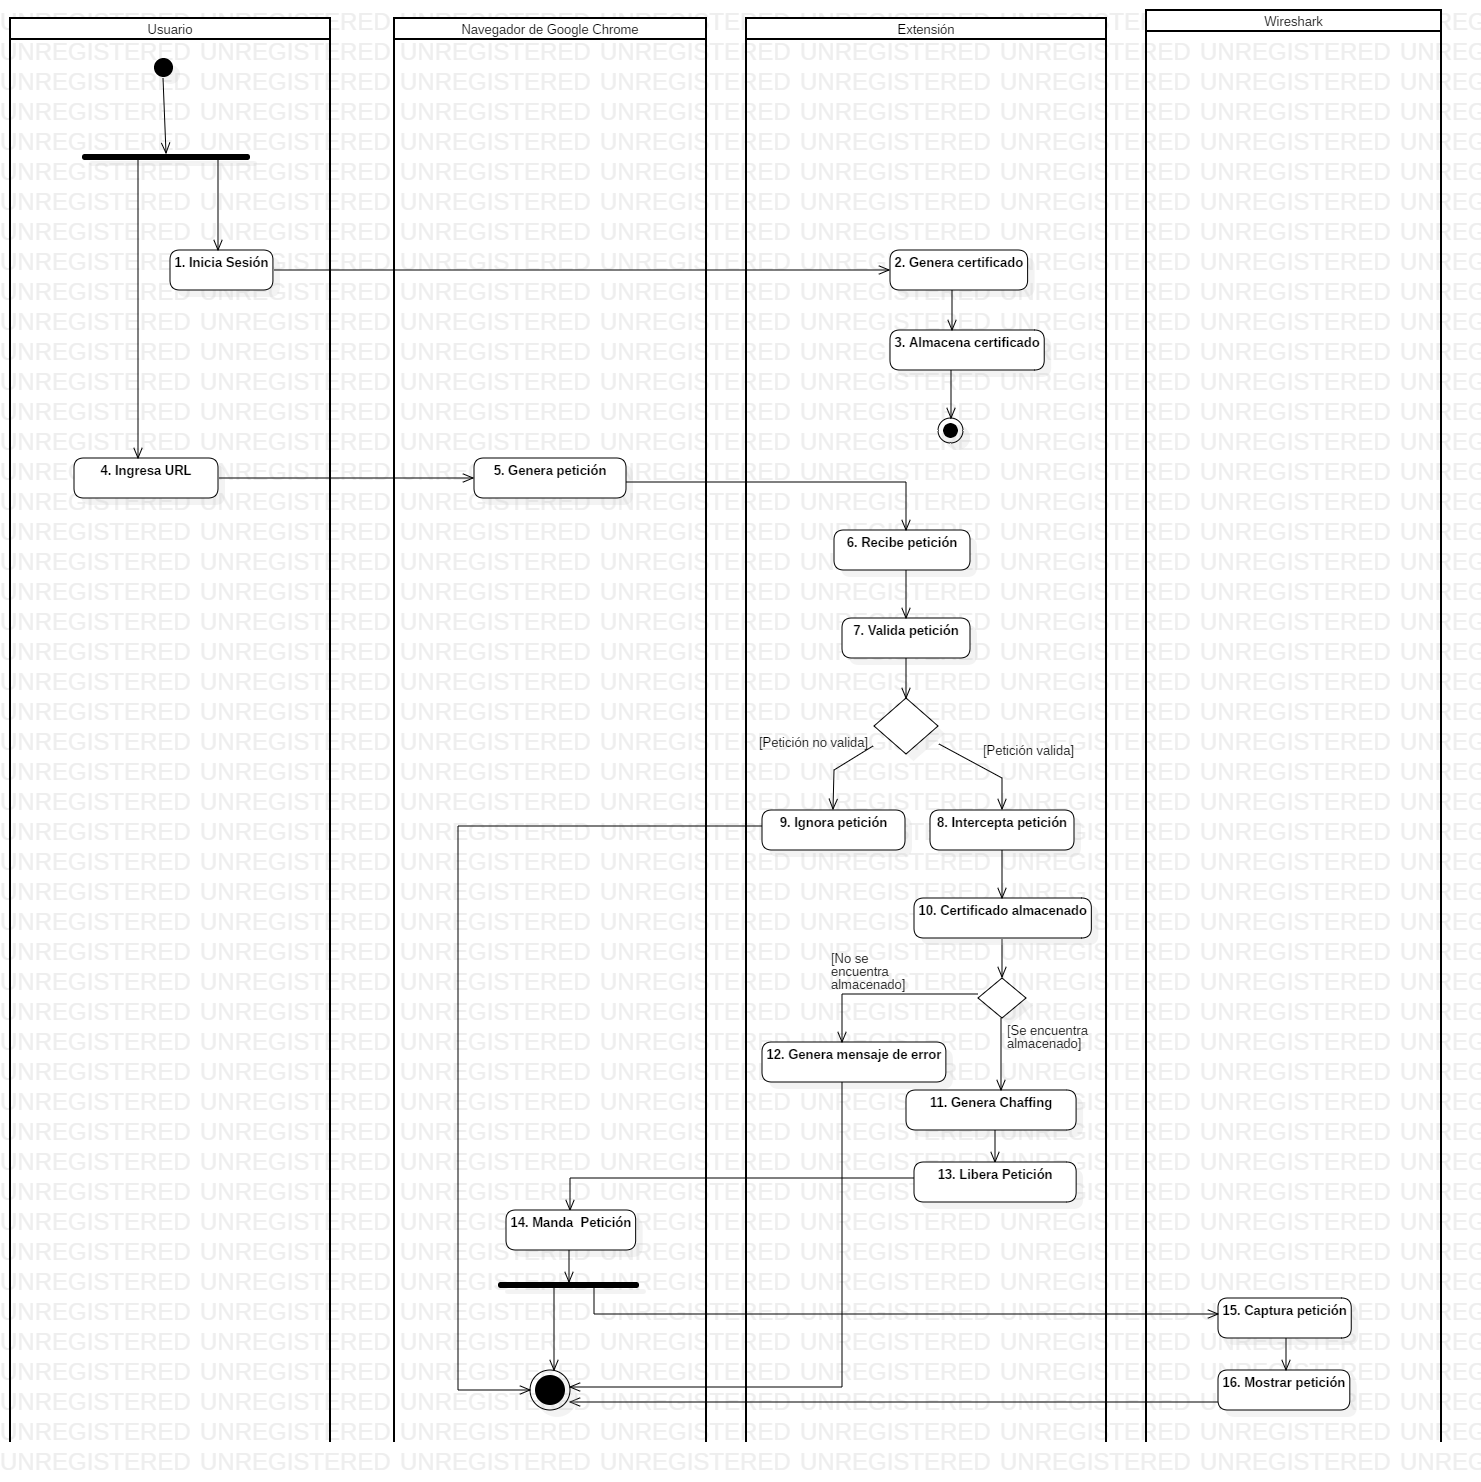
\includegraphics[width=15cm]{./imagenes/Desarrollo/Prototipo_2/DA_P2.png}
					\caption{Diagrama de actividades del Prototipo 2.}
				\end{center}
			\end{figure}
		
		\subsubsection{Descripción del diagrama de actividades.}
		Para este prototipo se han agregado más pasos para el diagrama de actividades, los cuales se describen a 
    	continuación.\\
    	Uno de los primeros pasos que debe hacer el usuario es iniciar sesión, esto con el fin de generar un certificado de acuerdo a los datos del usuario. Dicho certificado se almacena en la API de Google Chrome \textit{Storage}. \\
    	El otro camino a seguir por el usuario es realizar una búsqueda en el navegador, en la cual el navegador realiza la petición y la extensión recibe la misma. Modificándola siempre y cuando se encuentre un certificado guardado en \textit{Storage}. Si este proceso es válido, se genera el proceso de Chaffing y se libera la petición. El servidor se encarga de mandar dicha petición almacenada y en donde el analizador \textit{Wireshark} se encarga de capturar la petición para mostrarla.
			
		\subsection{Interfaz de usuario.}

		    \begin{figure}[H]
				\begin{center}	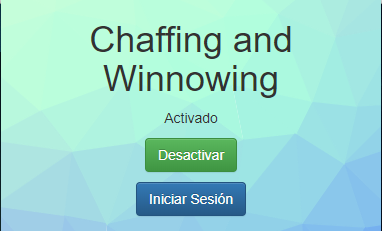
\includegraphics[width=9cm]{./imagenes/Desarrollo/Prototipo_2/UI_inicio.PNG}
					\caption{Pantalla inicial.}
				\end{center}
			\end{figure}
			  
		    \begin{figure}[H]
				\begin{center}	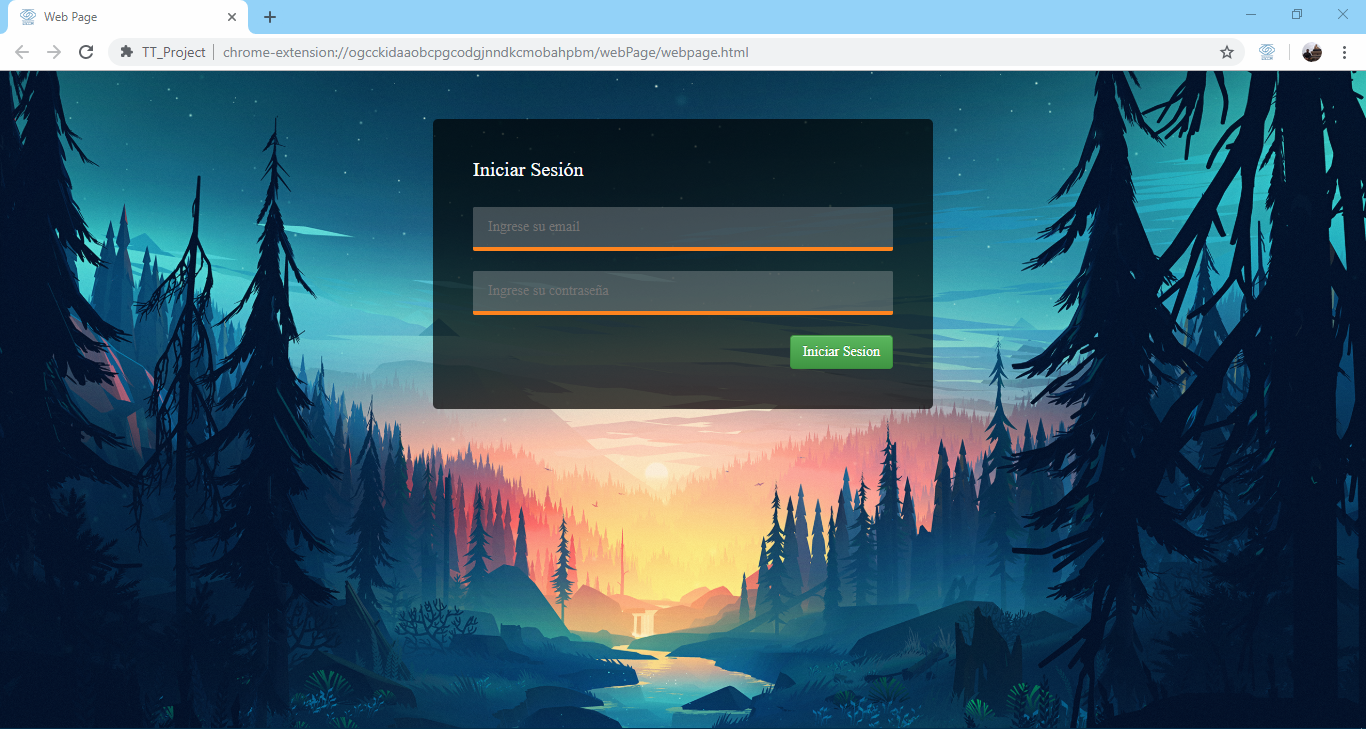
\includegraphics[width=15cm]{./imagenes/Desarrollo/Prototipo_2/UI_webpage.png}
					\caption{Tab de la extensión. Permite inicio de sesión}
				\end{center}
			\end{figure}
			
	    \subsection{Requisitos de diseño.}
			   En este apartado, se especificarán los requisitos de diseño para que el prototipo opere de forma correcta, de igualmanera se tiene por entendido que son necesarios los Requisitos del diseño del primer prototipo.
			   \subsubsection{Requisitos de ejecución de la extensi\'on}
			        Para poder ejecutar el prototipo dos es necesario contar con todo lo requerido para el prototipo uno y agregarle la interacci\'on con \textbf{jQuery 3.3.1 } y \textbf{Bootstrap} que son dos poderosos frameworks que corren sobre JavaScript y que nos permiten interactuar un poco mejor con el usuario haciendo la interfaz de la extensi\'on más amigable y entendible, estos ya se encuentran insertados en la extensión por lo que no es necesario que el usuario realice acción alguna.
			        Otros de los requisitos para su ejecución es contar con un \textbf{usuario y contraseña} válidos ya que ser\'an de suma importancia para el correcto funcionamiento del prototipo dos.
			     \subsubsection{Requisitos para el envío del código autentificador}   
			        Para este prototipo se considera necesaria los siguientes requisitos de diseño:
			        \begin{itemize}
			            \item \textbf{Código Autentificador} Archivo indispenzable en este prototito debido a que sin este es imposible acompletar el proceso.

			            %\item \textbf{Conexión con el servidor} al que queremos acceder ya que se enviará al servidor el codigo inyectado con \textit{Chaffing} .
			            \item \textbf{Botón para subir archivo} Este botón tendrá el propósito de darle al usuario la opción de escoger su certificado con el cual podrá ingresar a todas sus cuentas.
			            
			            \item \textbf{Botón de chaffing} Botón que generará un patrón de chaffing donde se aplicará en la petición HTTP, se inyectará el certificado de forma segura en la petición, y se simulará su envio al servidor.
			           
			        \end{itemize}
			        
			   
	
	%Para agregar una cita en el documento se usa \cite{refKey}, por automático los ordena conforme se van agregando
	\newpage
    \begin{thebibliography}{20}
	    \bibitem{ComparisonAuthenticationMethodsResources} Antonina Komarova, Alexander Menshchikov, “Comparison of Authentication Methods on Web Resources”, St. Petersburg National Research University of Information Technologies, St. Petersburg, Russia, 2016.
		\bibitem{refCriptology} Cryptology, Albrecht BeutelSpacher
		%https://books.google.com.mx/books?id=cTyBo6LvvMEC&printsec=frontcover&dq=cryptology&hl=es&sa=X&ved=0ahUKEwjcxLC9lP7gAhVNMqwKHXCBCn4Q6AEIKTAA#v=onepage&q=cryptology&f=false   
        
        \bibitem{refRamioAguirre} Seguridad informática y criptografía
        \bibitem{refHandBookOfAppliedCryptography} Menezes, Van Oorschot y Vanston, Handbook Of Applied Cryptography
        \bibitem{refSandra} Tesis de la profesora sandra
        \bibitem{refCriptografia} Maiorano, Ariel. Criptografía, Técnicas de desarrollo para profesionales.
		\bibitem{refJavaScript} https://www.dtic.upf.edu/~tnavarrete/fcsig/javascript.pdf 
		\bibitem{refElGranLibro} https://gutl.jovenclub.cu/wp-content/uploads/2013/10/El+gran+libro+de+HTML5+CSS3+y+Javascrip.pdf
		\bibitem{refSeguridadWeb} https://www.seguridad.unam.mx/historico/documento/index.html-id=17
		\bibitem{refRoboIdentidad}
		https://www.seguridad.unam.mx/historico/documento/index.html-id=16?fbclid=IwAR0u8WAXORvBxZ3H-aMzlBhd-6o7g8ycS88eRu7nY1t1XVtCufhEcQ7hWDs
		\bibitem{refSeguridadWebAguilar} Aguilar, A. and Hernández, A. (25 de Abril de 2014). Obtenido de Sugerencias de Seguridad para Sitios Web: http://www.seguridad.unam.mx/documento-id=1143
		\bibitem{refCookies}
		https://es.wikipedia.org/wiki/Cookie\_(informatica)
		\bibitem{refCookiesPersistentes}
		http://www.allaboutcookies.org/es/galletas/cookies-persistentes-utilizados-para.html
		\bibitem{refTiposdeCookies}
		http://www.gadae.com/blog/que-son-las-cookies-tipos-de-cookies-y-como-cumplir-la-ley/
		\bibitem{refFuncionalidadCookies}
		https://www.osi.es/es/actualidad/blog/2018/07/18/entre-cookies-y-privacidad
		\bibitem{refCryptography}
		http://www.dma.fi.upm.es/recursos/aplicaciones/matematica\_discreta/web/aritmetica\_modular/criptografia.html
		\bibitem{refChaffing}
		http://www.cs.bath.ac.uk/~mdv/courses/CM30082/projects.bho/2007-8/durongdej-r-dissertation-2007-8.pdf
		\bibitem{refRivestSeguridad}
		http://citeseerx.ist.psu.edu/viewdoc/download?doi=10.1.1.160.4853\&rep=rep1\&type=pdf
		\bibitem{refEncontrarLuegoAdivinar}
		S.  GOLDWASSER  ANDS. MICALI, “Probabilistic encryption,”Journal  of Computer andSystem Science, Vol. 28, 1984, pp. 270–299.
		\bibitem{refRivestMIT}
		https://people.csail.mit.edu/rivest/Chaffing.txt
		\bibitem{articuloAxel}
		© Springer International Publishing AG 2018
        A. Abraham et al. (eds.), Proceedings of the Second International
        Scientific Conference “Intelligent Information Technologies for Industry” (IITI’17),
        Advances in Intelligent Systems and Computing 679, DOI 10.1007/978-3-319-68321-8\_11
        \bibitem{filesystemmozilla}
        https://developer.mozilla.org/es/docs/Web/API/FileSystem
        \bibitem{opensslmillones}
            https://www.verisign.com/es\_LA/website-presence/online/ssl-certificates/index.xhtml
        \bibitem{openssl}
        https://www.globalsign.com/es/centro-de-informacion-ssl/que-es-ssl/
        \bibitem{refCryptoJs}
        https://code.google.com/archive/p/crypto-js/\#MD5
        \bibitem{refWireshark}
        https://www.wireshark.org/docs/wsug\_html\_chunked/ChapterIntroduction.html\#ChIntroWhatIs
	\end{thebibliography}	

\end{document}

